%https://excalibur-neptune.readthedocs.io/en/latest

\newchapter{Program Identity}{sec:PN}
%DESC %Audience for D3 are the developers, testers and support staff, plus 'occasional' manager.
%DESC %It is at a technical and precise level.
% Sommerville  - Preface
% Hewitt  - Program Name
\newsectionnobreak{Executive summary}{sec:exc-sum}

The program addresses key plasma modelling issues for reactor design.
This new software should become essential for designing optimal 
power-handling strategies at the tokamak first wall, both directly (via the 
simpler \papp s) and indirectly by improving detailed physical understanding of the 
often turbulent,  plasma-wall interaction.

This website was designed following the \nep \ workshop minuted as~\cite{y3re181},
and the related documents~\cite{y2d34,y3re314}.
to cover all aspects of the overall \nep \ package, as they emerge,
beginning with the initial concept, advancing to detailed design
of classes (objects) and  interfaces, and ultimately producing documentation
to ensure the software remains usable, maintainable and relevant for at least 30~years.

\subsection{Further information}
High-level project issues are covered by the project science plan~\cite{sciplan};
the \nep \ project is \exc \ funded~\cite{exch+eswebsite}. 
Distribution and use of the software is covered by the extremely
permissive MIT licence~\cite{MITlicense}, regarded as equivalent to the BSD3 licence.
Collaboration is encouraged, and there are many additional benefits of community membership
as set out below. Those interested in joining the community should
 email {\tt neptune@ukaea.uk} to establish a dialogue.


\subsection{Benefits of community membership}
The principal benefit is access to what should ultimately become a powerful 
and comprehensive software package for modelling tokamak edge plasma using
finite element and particle methods.
In addition members will also gain
\begin{itemize}
\item Access to reports as the community produces them, in the access-controlled github site~\cite{xpndocswebsite},
subdirectories {\tt reports} and {\tt reports/ukaea\_reports}.
These directories already include educational material on
\begin{itemize}
\item Finite elements
\item Surveys of current software
\item Surveys of current HPC machines and performance
\item Uncertainty Quantification
\item Aspects of software engineering, such as design patterns
\end{itemize}
\item Rights to attend workshops and shape the \nep\ software, announced in the Slack channel.
\item Right to attend project lectures on work performed by the community, and on
relevant background material such as the spectral/hp element method, announced in the Slack channel.
\item The {\tt tex} subdirectory~\cite{xpntexwebsite} contains bibtex databases to aid report writing in subdirectory {\tt bib} and graphics suitable for producing presentations
in subdirectories {\tt pics} and {\tt png}.
\end{itemize}
The Slack channel is `\#excalibur-neptune'. (The Slack communication
software is downloadable from \url{https://slack.com/}).

(Note that access to most \nep \ reports is restricted to community members.)

\subsection{Convention on use of IETF Keywords}
The RFC2119 subset of the Internet Engineering Task Force~(IETF) keywords~\cite{rfc2119}
is used throughout the website, unless stated otherwise. Such usage implies specific
meanings for ``MUST", ``MUST NOT", ``REQUIRED", ``SHALL", ``SHALL
NOT", ``SHOULD", ``SHOULD NOT", ``RECOMMENDED",  ``MAY", and ``OPTIONAL"
\emph{when} the words are capitalised.

%

% Sommerville  - Preface from Fig. 4.17 (p.128) The structure of a requirements document
% Hewitt  - Program Name
\hspace{-30mm}\begin{table}[h]
\sffamily
\begin{center}
\textbf{\textsf{UKAEA REFERENCE AND APPROVAL SHEET}}
\begin{tabular}{||p{5.7cm}|p{4.7cm}|p{5.0cm}||}
\hline
\hline
& Client Reference: &  \\
\hline
& UKAEA Reference: & \culhamshorttitle \\
& & \\
\hline
& Issue: & \culhamissueno \\
\hline
& Date: & \culhamdateb \\
\hline
\multicolumn{3}{||l||}{} \\
\multicolumn{3}{||l||}{Project Name: ExCALIBUR Fusion Modelling System} \\
\multicolumn{3}{||l||}{} \\
\hline
\end{tabular}
\begin{tabular}{||p{3.3cm}|p{4.6cm}|p{3.5cm}|p{3.6cm}||}
\hline
& Name and Department & Signature & Date \\
\hline
Prepared By: & \culhamauthor & N/A & \culhamdate \\
& \culhamauthora & N/A & \culhamdate \\
& \culhamauthord & N/A & \culhamdate \\
& \culhamauthorb & N/A & \culhamdate \\
& \culhamauthorc & N/A & \culhamdate \\
& & & \\
& CD & & \\
\hline
Reviewed By: & \culhamauthor & 
\includegraphics[width=3.0cm]{./corpics/blanksign.png}& \culhamdatea \\
& & & \\
& Technical Lead & & \\
\hline
Approved By: & \culhamauthor  & 
\includegraphics[width=3.0cm]{./corpics/blanksign.png} & \culhamdateb \\
& & & \\
& Technical Lead  & &\\
\hline
\hline
\end{tabular}
\end{center}
\end{table}


\newchapter{Business Design}{sec:BD}
% sections 1 to 7 of Hewitt  - Business Design
% Sommerville  - Introduction
\begin{enumerate}
\item  {\bf CAPABILITIES}

The \nep \ package will be capable of efficiently contributing `actionable' results regarding
the first wall to the reactor design process, specifically by speedily modelling the power deposited by the plasma
\begin{itemize}
\item subject to uncertainty quantification~(UQ)
\item using a modular suite of compatible components of minimal necessary complexity 
so as to ensure a workflow for rapid design,
capable when needed of involving the latest high performance computers (HPC)
\end{itemize}
In addition, the package will facilitate  research into edge plasma physics by
\begin{itemize}
\item its ease of use, providing a suitable DSL for `high-level' usage in Python/Julia to enable
intuitive additions to existing models or the incorporation of new models, whereby
equations may be defined using \LaTeX \ as explicit PDEs or as Lagrangians, %, as Lie derivative.
and novel initial conditions imposed and new boundary conditions applied
\item its ease of modification and development, by
providing a set of well-defined objects/classes for tokamak plasma physics
\item ease of incorporation of its component software into other physics packages
\item offering a careful automatic control of numerical error
\end{itemize}

\item  {\bf STRATEGIC FIT} % - to UKAEA mission

{\bf National}: The \exc \ project is of national importance to UK government
(represented by the BEIS dept.)  to demonstrate
how to produce software that can exploit all the latest, most powerful hardware
for scientific computation.  The Fusion Modelling System~(FMS) is one
of \exc 's principal use cases, for which project \nep \ will explore efficient development of
new software for the Exascale.

%UKAEA researches fusion energy and related technologies, with the aim of positioning
%the UK as a leader in sustainable nuclear energy.
{\bf UKAEA}: The software will facilitate world-leading R\&D into fusion energy by UKAEA physicists and
engineers, underpinned by external collaborators with a wide range of expertise.
Its research contribution will be to improve detailed physical understanding
of the often-turbulent plasma-wall interaction. Development of tokamak reactors will
be facilitated if Exascale machines can be seamlessly integrated into the design workflow.
\item  {\bf BUSINESS DRIVERS} % - why are we doing this?

Optimal power-handling at the wall will be critical for fusion reactors to be able to
deliver sustainable fusion energy to the grid economically, if at all.
%Accurate detailed modelling requires large computing resources,
Rapid exploration of parameter space is important to understand and optimise
reactor designs, yet the existing software available to UK is dated so that it
require years of experience to use well and is not suited to the latest HPC.
Its replacement should remove a major handicap in the race to produce reactor designs.
\item  {\bf ASSUMPTIONS} % regarding available funding

Funding of approx.\ $\pounds$\,5\,M over $5$~years has been made available to UKAEA via the Strategic
Priorities Fund under its \exc \ programme to ready the UK for the Exascale era of computing.
It is expected that further development of the \nep \ software will be funded at a similar if
somewhat smaller level after 2025.
%\item  {\bf (CONSTRAINTS)} % laws and regulations)
\item  {\bf RISKS} %  if resources not available

Funding is via UK government and does not depend on the international situation.
\item  {\bf IMPACTS} % new processes, training needed

The new software should enable much faster iteration in respect of engineering design of the first wall
of tokamak reactors. It should save much time and effort in the modelling of
tokamak edge plasma physics. Generally, it should greatly reduce the training and computer time
needed to obtain results compared to the existing software. There should also be benefits to
UKAEA's wider relationships with the Eurofusion E-TASC programme and with ITER.
\item  {\bf STAKEHOLDERS} % who will win or lose by good or bad outcome

The successful outcome of the project should be a plus for the UK, UKAEA and most employees.
The only losers will be those UKAEA staff and contractors who have devoted often years of
their working lives to the dated software that \nep \ is
designed to replace, and will undergo a loss of status in consequence. However, their physics skills
and understanding will be valuable for guiding the \nep\ development to produce maximum
benefits, hence they should soon recover position within UKAEA.
\item  {\bf GOVERNANCE} % committees

The \nep \ project is overall governed by the UK governance known as PRINCE2~\cite{prince2,prince2wiki}.
which demands oversight by a local committee known as a project board.
Finance is subject to the usual UKAEA procedures and controls.
The \nep \ project is further subject to
reporting to UK Met Office as part of wider \exc \ activities, whence there is a
second layer of PRINCE2 oversight.

The planned technical activities are outlined in the Science Plan~\cite{sciplan},
it and all  major changes and refinements are subject to external refereeing,
following the \exc \ procedures drawn up by UK Met Office consistent with the 
demands of the UK Strategic Priorities Fund~\cite{SPF}.
External procurements similarly follow the \exc \ procedures drawn up by UK Met Office.
\end{enumerate}

%There are
%deficiencies in the existing plasma physics software base for modelling the
%tokamak edge which should be addressed, and there is the question of how best to meet them. There is the issue of
%whether to exploit opensource software, and if so how best to do so. Factors such as
%future-proofing, speed of code execution, the need for uncertainty
%quantification,
%the interaction between different packages for CAD, meshing and physics codes are
%accounted for in the discussion. The avoidance of ``heroic computing" in favour of UQ
%could lead to considerable simplification in choosing a way forward, probably without
%any significant long-term drawbacks.

% sections 1 to 7 of Hewitt  - Business Design
% Sommerville  - Introduction

\newchapter{Requirements Baseline}{sec:RB}
The Requirements Baseline (RB) expresses the user requirements for the software.
%The Interface requirements document (IRD) expresses the customer's interface
%requirements for the software to be produced by the developer.
%This document is part of the requirements baseline.
% Hewitt  - Use Cases
% Sommerville  - User requirements definition
% Smith  - Problem Statement
% Smith  - Requirements  - Introduction
% Smith  - Requirements  - Requirements  - Functional Requirements
% Smith  - Requirements  - General System Description  - User Characteristics

The largest input to the process, representing UKAEA Tokamak Science
Department appears under Technical Specification~\Sec{TS}, so that it may
be accompanied by a detailed response. Instead, there is presented an appreciation
of the properties of the plasma edge in \Sec{props}.

The Departmental input, although it deals with other aspects of the specification,
focusses more on the physical processes to be modelled and the approaches likely to
be required. The following \Sec{RB2} records interactions with UKAEA Engineers, although
a subsequent meeting clarified that the main demand for \nep\ at that time was that it be a
modular, component-based design, equally suitable for integration into ANSYS OptisLang$^{TM}$
as VECMAtk (with more detailed requirements likely to follow when the software became more developed).
Thereafter the  next \Sec{use_case}  contains use cases, followed by \Sec{general-remarks}
describing general requirements deducible from the use cases.

\newsection{Physical properties of the edge plasma}{sec:props}
%\section{Physical properties of the edge plasma}\label{sec:props}
The following scrape-off layer (SOL) parameters (including decay lengths) are for the
L-mode scrape off layer in MAST~\cite{Mi13Expe}.
For MAST,  with the standard notation,
$R_0=1.6$\,m, $B_T \approx 0.6$\,T, $I_\phi \approx 400$\,kA and
$a=0.6$\,m, values which imply that the poloidal field at the
plasma edge $B_p \approx 0.1$\,T.
The main result of the paper~\cite{Mi13Expe} is that the decay length of the power
deposition at midplane is $\lambda_q \approx 2$\,cm (range $1-3$\,cm)
and $P_{tot} \approx 350$\,kW.

Unless stated otherwise, the derived length, timescales and speeds are derived from
formulae and graphs in Wesson's book~\cite[Chap 10]{wesson}.
The derived quantities have been checked against SI formulae
in~\cite[Table 2.2]{miyamoto}, and also compared with those
listed in~\cite[Appendix]{Xu10Inte}. It is worth noting that although
the latter table describes the SOL of JET (and in addition its separatrix and pedestal),
JET values are typically within a factor of~$2$ of those for MAST, hence similar
numbers could be inferred for reactor designs.

\subsection{Typical discharge}

The edge values found experimentally are 
$T_e \approx 10$\,eV, $T_i \approx 20$\,eV, $n \approx 3 \times 10^{18}$\,m$^{-3}$.
These imply that the Coulomb logarithm $\Lambda \approx 12.5$, and
the flow speed~$U_d \approx 10^5$\,ms$^{-1}$ may be estimated using
$P_{tot}= 2 \pi R \lambda_q n (T_e+T_i) U_d$.
Sadly there appears to be no reliable determination of the neutral density~${\sf n}$.
(Note use of different font to distinguish neutral density from plasma density.)

\subsection{Length scales}

Debye length $\lambda_D \approx 10^{-5}$\,m. \\
Electron Larmor radius $\rho_{te} \approx 7 \times 10^{-5}$\,m. \\
$\rho_{ti} \approx 40 \rho_{te} \approx 4$\,mm. \\
Mean free path for electrons $\lambda_{emfp} \approx 1$\,m (parallel to field).

\subsection{Time scales}

%$\tau_e \approx 2 \times 10^{-8}$\,$s$.
Collision frequency (electrons with ions) $\nu_e \approx 3$\,MHz, $\tau_e \approx 3 \times 10^{-7}$\,s~\cite{NRLpf07}. \\
Plasma frequency $f_{pe} \approx 15$\,GHz, $\tau_{pe} \approx 7 \times 10^{-11}$\,s. \\
$f_{pi} \approx 0.4$\,GHz, $\tau_{pi} \approx 3 \times 10^{-9}$\,s. \\
Cyclotron frequency based on $B_p=0.1$\,T, $f_{ce} \approx 2.8$\,GHz, $\tau_{ce} \approx 4 \times 10^{-10}$\,s. \\
$f_{ci} \approx 1.4$\,MHz, $\tau_{ci}\approx  7\times 10^{-7}$\,s.

\subsection{Speeds}
Electron thermal $c_{se} \approx 1.2 \times 10^6$\,m$s^{-1}$. \\
$c_{si} \approx 4 \times 10^4$\,m$s^{-1}$. \\
Alfven speed using $B_T$ is $U_A \approx 10^7$\,m$s^{-1}$.

Collisionality parameter $\nu^{*}_c = \frac{q_e^4}{3 m_p^2\epsilon_0^2} L_0 n_0 /C_0^4$ \\
(note that $\frac{m_p^2\epsilon_0^2}{e^4}=\frac{1}{3}\;s^4 m^{-6}$.)\\
Taking $L_0 \approx 10$\,m, $n_0=n$.  Squared sound speed $C_0^2= T_i (|e|/m_e) (m_e/m_i)$, $C_0 \approx 3 \times 10^4$\,m$s^{-1}$, implies  \\
Collisionality parameter $\nu^{*}_c \approx 30$. \\
Peclet number $\approx 0.4 \nu^{*}_c \approx 10$, but turbulent coefficients$\approx1$\,m$^2$s$^{-1}$
will generally give a smaller value.

Resistive diffusion $\eta_d=15$\,$m^2 s^{-1} \propto T_e^{-3/2}$. \\
(Note that there is a notational clash with~$\eta$; fusion physics and astrophysics
differ by a factor~$\mu_0$, so that $\eta_d=\eta(\mbox{fusion})/\mu_0$.)

\subsection{Applicability of Fluid Models}\label{sec:applmhd}
A key requirement for fluid models is that collision times should be much less than
the timescale of interest, which as the preceding subsections show is true, except in the case of
$\tau_e$, the electron-ion collision time, and for the electrons more generally
for dynamics along the field-lines. The ion gyroradius is also uncomfortably large
compared to quantities of interest. Note that $\tau_e$ is the longest timescale
in the classical picture of approach to a single fluid picture of plasma, other
timescales, including the timescale for momentum to equilibrate, are shorter.

Single fluid MHD is widely used in astrophysics consistent with the eloquent advocacy
by Priest and Forbes~\cite[\S\,1.7]{priestforbes}. They point out that ideal MHD
is consistent with the drift ordering, despite confusion caused by the easy possibility
to misinterpret
Hazeltine and Meiss~\cite {hazeltinemeiss} on the subject. (The point is that
although MHD treats a faster timescale, it is valid on longer timescales, provided
relevant smaller/slower terms are retained.)
Moreover, SOL timescales involving filaments are fast, witnessed by the fact that
the ion gyro-frequency is used as normalisation for electrostatic models in~\cite{Mi12Simu},
which from \Sec{props} is a not too dissimilar timescale~$10^{-7}\,s$
to the Alfven timescale based on the poloidal field~($1$\,cm/$10^6 \approx 10^{-8}$\,s).
Later, Freidberg~\cite{freidberg}
showed that, at least in directions perpendicular to~${\bf B}$, the dynamical MHD equation
applies to a more general `guiding centre' plasma. The situation may be summarised
by saying that complexity lies mostly in the transport (diffusive) terms
as these attempt to account for low collisionality, finite Larmor radius (FLR) etc.

Perhaps fortunately, the terms predicted by kinetic theory will usually be small
(except for the electrical conductivity) compared to the turbulent transport
expected on the basis of both observation and theory of the SOL plasma. The
simplest way to account for turbulence is to assume ad-hoc isotropic, uniform `eddy'
diffusivities in addition to the usual fluid advection terms.
Lastly, in a simple extension of MHD, large~$\tau_e$  is accounted for by allowing
the electrons and ions to have different temperatures, consistent with observation.
Effects due to the presence of a large neutral population in the SOL
could well be significant, see next \Sec{neuts}.
However neutrals are mainly expected to act as a sink of momentum and energy.

\subsection{Effect of Neutrals}\label{sec:neuts}
Formulae for a weakly ionised plasma are given in the Plasma Formulary~\cite{NRLpf07}.
The collision cross-sections for electrons and ions respectively from~\cite{Ha91hydr}
are $\sigma_s^{e|0}= 10^{-19}$\,$m^2$ and
$\sigma_s^{i|0}= 4 \times 10^{-19}$\,$m^2$.
Hence, the collision frequencies for electrons and ions respectively are
\begin{equation}
\nu_{e{\sf n}}= 1.2 \times 10^{-13} {\sf n},\;\;\; \nu_{i{\sf n}}= 2 \times 10^{-14} {\sf n}
\end{equation}
where ${\sf n}$ is the neutral density.
(Note use of different font to distinguish neutral density from plasma density.)
If ${\sf n}=n$ is assumed, then
the corresponding SOL collision times are
\begin{equation}
\tau_{e{\sf n}}= 3 \times 10^{-6} s,\;\;\; \tau_{i{\sf n}}= 2 \times 10^{-5} s
\end{equation}
so that the number of collisions experienced by a typical SOL ion
before it hits a PFC is small.
Nonetheless, since $1/m_e \gg 1/m_i$, $D_e \gg D_i$ and the
diffusion coefficient for both electrons and ions is numerically large
\begin{equation}
D_A \approx (1+\frac{T_e}{T_i}) D_i \approx \frac{10^{23}}{{\sf n}}
\end{equation}

The parallel electrical diffusivities are different,
for electrons and ions respectively these are
\begin{equation}
\eta_{e {\sf n}\parallel} =4 \frac{{\sf n}}{n},\;\;\;
\eta_{i {\sf n}\parallel} =0.5 \frac{{\sf n}}{n}
\end{equation}
The implication from the formulae in~\cite{Le06emer} is that 
the value for $\eta_{e \parallel}$ combines additively with the usual
Spitzer value in a more
highly ionised plasma. Assuming ${\sf n} \approx n$, however the correction
is seen to be an increase of $4$ in $15$\,$m^2s^{-1}$, i.e. only about~$25$\,\%.

Arber~\cite{Le06emer,Ar07Emer} further points out that
according to the Formulary~\cite{NRLpf07},
in a weakly ionised plasma
the conductivity is greatly reduced (and the magnetic diffusivity
correspondingly enhanced) in directions normal to a strong magnetic field.
Typically for Braginskii theory, the
factor is $x_e^2$ for the perpendicular direction and $x_e$ for
the other direction, where
\begin{equation}
x_e=\frac{2\pi f_{ce}}{\nu_{e{\sf n}}} \approx \frac{8 \times 10^{23}}{{\sf n}}
\end{equation}
For ${\sf n}=n=3 \times 10^{18}$, these are huge increases. However it is worth
noting that if the electromagnetic potential representation is invoked, so that
\begin{equation}\label{eq:E}
{\bf E} = -\nabla \Phi + \frac{\partial {\bf A}}{\partial t}
\end{equation}
then, in the direction parallel to~${\bf B}$, neglecting the gradient of
electric potential~$\Phi$
\begin{equation}\label{eq:A}
\frac{\partial  A_{\parallel}}{\partial t}=\eta_{e {\sf n}\parallel} J_{\parallel}
\end{equation}
Thus the enhanced diffusivities need not signify if this equation is used for
magnetic field evolution, although applying a gauge condition on the potentials
may become difficult in complicated 3-D topologies.



\newsection{Engineering Requirements Baseline}{sec:RB2}
\subsection{Introduction}\label{sec:RB2_intro}
This set of requirements is based on four main sources, namely
\begin{itemize}
\item presentation by Chris Jones~(CJ) at the \nep\ internal workshop on 16 December~2019
\item points made in an email by Michael Kovari~(MK) dated 19 December~2019
\item interview with Zsolt Vizvary~(ZV) on 20 December 2019
\item use by author~(WA) of \F{SMARDDA-PFC} software in tokamak reactor design 2016-2020
\end{itemize}

A significant part of CJ's talk concerned calculations of stress in `contact' problems and in
tokamak-relevant materials, particularly those to be used in and adjacent to the
first wall. Mention was also made of nuclear heating and activation effects in the wall, and
their effect on its strength. Since \nep \ is primarily intended as a plasma modelling tool, this
material is neglected here except insofar as it has implications for \nep \ interfaces.
Similarly ZV has as high priority, a capability to do magnetic equilibrium calculations so
as to be able to calculate electromagnetic stresses in the wall.
CJ emphasised that engineering design at UKAEA makes heavy use of the ANSYS$^{TM}$
software for multiphysics calculations, and that since plasma effects including neutral beams
and fast ions are not part of any standard finite element toolkit, particular consideration should 
be given to interfacing \nep \ to ANSYS macros and ACT~(Python scripting for ANSYS).
CJ stated that ANSYS had been implementing additional physics very slowly, on a timescale of decades,
and there is anyway not a satisfactory licence model for using ANSYS on HPC,
nor any to be expected soon.

Although the \F{SMARDDA} software takes as input general surface triangulations, which may therefore
represent arbitrary surface topologies, \F{SMARDDA-PFC} calculates power deposition on the basis
of a simple, empirical physical model of transport from the outer midplane.
The errors in the model are frequently unquantifiable, given an absence of relevant experimental data,
notably when `small' limiters are proposed, where `small' implies that many lines of magnetic field make several
mid-plane passes before interacting with the limiter(s). The \nep \ software should provide a better
physical model to enable (1) calculation of the midplane profile of power `deposition' and associated
parameters such as the e-folding length~$\lambda_q$, when an exponential is fitted, and
(2) an assessment of the accuracy of the whole \F{SMARDDA} surrogate model in a wide range of
existing and novel configurations.
 

\subsection{Overall Capabilities}\label{sec:RB2_overall}
Chris Jones has been led to dream of a \\
\emph{Whole-system full-physics digital twin available for real time in-silicon simulation and experimentation}\\
but recognised that a more immediately realisable prospect was integration of plasma software into ANSYS
Workbench$^{TM}$.

\begin{enumerate}
\item Simulations must be of known, improved accuracy, so that the performance of the
built designs can be enhanced without sacrificing safety.
Thus the code and data structure should support mesh convergence studies, and be `physics aware' as described
in \Sec{RB2_physmod}.
\item The power load should be easily transferable to ANSYS for stress, heat transfer and other  multi-physics analysis.
\item The software should be easy to couple to other physics packages produced within the fusion
community such as \F{RACLETTE} and \F{ERO} for erosion calculations, \F{LOCUST} and \F{SMARDDA-PFC} for power
deposition by particles, and neutronics software such as \F{MCNP}.
\item The software should be designed to support easy production of statistics from ensemble calculations,
even when costs limit the size of the ensemble. The ensembles should be able to include different model
selections as well as different parameter choices.
\item The software should be easy to use on HPC, eg.\ through cloud-based services, where 
it should be resilient to  network bottlenecks.  Its performance
should scale well and  not depend on the OS used.
\item The software should be able to exploit GPGPUs.
%\item The software should be capable of calculating both (quasi-)static and transient behaviour
\item The software should use well-defined standard, open formats for both input and output of data.
\item The code should be easy to extend, without writing new code. Thus a user should be able to
extend (at least virtually) a data structure to include a new parameter, and add a new physical effect.
\item The following aspects of the software should be open: 
\begin{enumerate}
\item data structure requirements and documentation
\item code and documentation
\item test cases and their documentation
\item all results and their documentation
\end{enumerate}
\end{enumerate}

\clearpage
\subsection{Physics Model}\label{sec:RB2_physmod}
The software should be automatically `physics aware', ie.\ it should
\begin{enumerate}
\item be able to test the physical assumptions and orderings used, perhaps by calculations at randomly placed points, and
when this is impossible, to
produce output to enable an independent person to check against a separate code.
\item be intelligent enough to switch to a simpler assumption
when appropriate or when instructed to do so, for example by using classical
transport coefficients when they apply.
\item be able to test the level of detail used.  For example, the code  (1) 
could carry out an ensemble calculation using a simplified model of radiative loss,
and then check the results in a much shorter time against a fuller model using
a sampling technique, (2)  be able to identify
automatically that a fully 3-D field calculation with say 12 or 18 discrete TF
coils has produced a toroidally axisymmetric field in the vacuum vessel.
\item be able to simulate transient behaviour, being able to determine an initial approximate quasi-static solution, then
depending on the length of the simulation relative to physical timescales of interest, perform
either an implicit or an explicit calculation.
\item distinguish physical time from pseudo-time when relevant, eg.\ in an implicit calculation.
\item be able to handle incompatible timescales for bulk and local behaviour, eg.\ account for particle effects on overall flow.
\end{enumerate}
\clearpage
\subsection{Physics Capabilities}\label{sec:RB2_physcap}
The software should be able to 
\begin{enumerate}
\item compute the total power load on solid walls, due to plasma, fast ions and neutral beams
\item compute the production of impurity species by first wall melt and evaporation
\item compute heat conduction in first wall coatings in contact with the plasma
\item perform high frequency electrical and magnetic analysis, accounting for skin effects
\end{enumerate}
%\clearpage
\subsection{Geometry}\label{sec:RB2_geom}
\begin{enumerate}
\item The software should be able to account for the effect of changes to geometry caused by radiation swelling,
erosion and deposition due to plasma interaction, and corrosion.
\item The code should allow periodic toroidal boundary conditions.
\item The software should be able to handle 0-D, 1-D, 2-D and 3-D representations of the same plasma pulse,
transferring between the different representations.
\item A related example concerns the recognition of field axisymmetry as in \Sec{RB2_physmod}.
\item Convexities in the surface, even sharp corners capable of causing singularities in the magnetic and stress fields, should
be treatable by the software.
\end{enumerate}


\newsection{Use Cases}{sec:use_case}
\subsection{Use Cases: Tokamak edge physicist}\label{sec:edge-boundary-tokamak-physicist}

They are early career, and to progress they need to build a professional
reputation by publishing papers, supporting UKAEA's research programmes
and supervising students. They are a competent developer and experienced
HPC user, though they do not gain any credit directly from developing
software.

In their research work, they study different models for the tokamak
edge, and so require code flexibility and a user-friendly DSL to allow
them to rapidly prototype different equation sets. This work would
require quick iterations -- perhaps 5 minute simulations performed on a
desktop. They will also develop their own algorithms and add
infrastructure to the code. While they will do this with an
understanding of performance implications, they would expect to perform
these developments at a higher level that raw performance loops (but at
a lower level than the physics model).

They would expect to contribute their changes back to a community
repository, and also to benefit from changes that other code users have
made. They would be involved in the community -- perhaps raising issues,
making and reviewing git pull requests, answering queries, and having input into
future code releases -- but would not be involved ``project management''
tasks, like maintaining the repository.

They will also value a user-friendly interface and active user community
when it comes to working with their students. In this context it is
valuable to have software that will run at a high level and produce
sensible results without needing to specify the details of the
implementation. This allows the student to learn about physical systems
without simultaneously having to learn the details of numerical
implementations. The active community allows their student to get
support and ask (perhaps trivial) questions without being dependent on
their supervisor.

Finally, in support of experiments, they will need to perform
high-fidelity simulations of tokamaks. These will be highly
computationally expensive, either because they are high-resolution
simulations of specific shots, or because they are parameter scans or UQ
campaigns. The simulations will be long-running, perhaps in the range of
a week to a few months, on whichever HPC system that they have access
to. The software must therefore be performance portable in order to
facilitate high performance on a range of systems. The software also
needs to be robust to numerical instabilities, hardware node failures,
etc, as one may not have the resource allocation to repeat failed runs.

\subsection{Use Cases: Engineers}\label{sec:use-cases-engineers}

\emph{As a thermomechanical engineer I:}

\begin{itemize}
\item work with a large range of open source and proprietary codes which
  requires bindings to other tools, eg\.:

  \begin{itemize}
  \item FMU
  \item Python (Jupyter and regular)
  \item OptiSLang
  \item Twinbuilder
  \end{itemize}
\item work with CAD software to generate geometries which I want to
  propagate through my workflow.
\item am interested in heat fluxes in all forms: from time and space
  averages to high resolution 3D time and data.
\item need to be able iterate on designs quickly and in an automated way.
\item am neither an HPC expert nor a plasma / tokamak physicist.
\end{itemize}

\emph{and I want to:}

\begin{itemize}
\item know, given a sensible physics model provided by other experts, what
  the transient peak and average heat loads are on plasma facing
  components.
\item not have to understand software dependencies and be able to install and
  run easily eg.\ ``in the cloud''.
\item be able to configure the software to undertake parameter scans.
\item have a handle on the sensitivity of the solution to the inputs and
  sources of error / uncertainty.
\item be able to re-use the spatio-temporal heat fluxes as a model in more
  thermo-mechanical calculations. This means:

  \begin{itemize}
  \item reading in the solution after the calculation.
  \item using a fit to the data in the form of eg.\ a reduced order model of
    the heat fluxes, surrogates etc.
  \item being able to export CAD geometries and import solutions back into
    engineering tools eg.\ ANSYS.
  \end{itemize}
\item have reproducible workflows to save and share with colleagues
  (eg.\ databases of inputs / outputs / config).
\item export results flexibly to inter-operate with multiple surrogate
  frameworks.
\item be in the loop with development process so it is possible to keep other
  workflows up to date.
\end{itemize}

\emph{This would mean I can:}

\begin{itemize}
\item design components with colleagues within eg.\ STEP.
\item make use of the \nep\ software in combination with proprietary tools that engineers
  know inside out.
\item be insulated, to a sensible extent, from the complexities of the
  numerics, plasma physics and HPC.
\end{itemize}

\subsection{Use Cases: Particle Specialists}\label{sec:use-cases-particle-specialists}

\emph{As a particle specialist I:}

\begin{itemize}
\item am very familiar with particle based methods.
\item may not be familiar with FEM implementation details but have a working
  understanding of the approach.
\item may not be familiar with low level languages.
\item may not be familiar with HPC hardware and architectures.
\item understand how to describe complex physical processes such as
  radiation, recombination, ionisation, charge exchange using both
  particle and FEM data.
\item may not have applied UQ techniques before but may have an
  understanding of distributions/ensembles from statistical mechanics.
\end{itemize}

\emph{I want to:}

\begin{itemize}
\item describe particle based operations both collectively and per particle,
  eg.\ :
\begin{itemize}
\item creation and deletion of particles potentially from complex
  distributions.
\item computation with particle data - per particle and collectively.
\item identification of groups of particles.
\item representation of arbitrary per particle data.
\end{itemize}
\item visualise particle and FEM data - snapshots and trajectories.
\item create new finite element functions on appropriate function spaces.
\item add source/sink terms to governing equations (solved with FEM).
\item define particle source and sink regions using the simulation domain
  geometry.
\item define regions of interest, eg.\ surfaces, as part of diagnostics.
\item identify particles near surfaces/points/volumes of interest.
\item create and use global data structures for computation,
  eg.\ diagnostics.
\item represent particle data as FE functions:

  \begin{enumerate}
  \def\labelenumi{\arabic{enumi}.}
  \item through pointwise projection.
  \item line integration over particle trajectory.
  \end{enumerate}
\item use non-trivial functions in my loops, eg.\ erfc, gamma.
\item define functions using expansion coefficients, eg.\ ionisation rate
  function approximated by an exponential expansion.
\item evaluate these functions using both particle and FEM data.
\item describe pairwise operations that implement physical processes.
\item describe and sample from non-trivial statistical distributions.
\item perform simulations in a reproducible manner.
\end{itemize}

\emph{So that I can:}

\begin{itemize}
\item use particles as a kinetic description for plasma and neutrals.
\item represent highly-collisional regimes by fluid approximations.
\item describe plasma-neutral and plasma-plasma interactions.
\item use abstractions/DSLs to write once, run anywhere as much as possible.
\item experiment with models quickly and efficiently.
\item perform ensemble computations and averages.
\item perform UQ and verification.
\end{itemize}

%This is an attempt at a profile of a certain class of \nep \   user stating 
%what might be reasonable expectations of the code and its interface.
\subsection{Use Cases: Finite Element Background}\label{sec:use-cases-finite-element-background}

I am a user with perhaps some grasp of plasma physics but with a more extensive 
knowledge of finite-element software (I might be an experienced user / 
developer of Nektar++).  My background may be either physics or engineering; I 
may be a new recruit to the \nep \ team and needing to learn the code with a 
view to taking a future role as a \nep \ developer.

I need the interface / DSL to provide access to typical FEM parameters eg.\ 
choice of intra-element basis functions and their polynomial order, continuous 
/ discontinuous Galerkin, choice of numerical flux, stabilization options; also 
whether diffusion and advection terms are explicit or implicit.  In line with 
eg.\ Nektar++ I expect the choice of time-stepper to be largely ``orthogonal'' 
to most details mentioned above (the exception is explicit / implicit choice).  
I would like the option to specify the timestep in terms of the CFL number.
In addition I require control 
over relevant meshing parameters eg.\ element spatial density and approximation 
order of any curvilinear elements.
I would like the DSL to be able to generate a range of regular meshes 
internally (at least for trivial cases eg.\ boxes meshed with quads).

I should like some simple, physically-motivated canonical examples that might
assist with learning plasma physics.

I expect the performance of the code to be at least commensurate with other FEM 
packages eg.\ Nektar++ and to remain so going forward (and obviously must be 
scalable to the latest hardware, which means foreseeably an efficient GPU 
implementation, supporting ideally NVidia, AMD, and Intel Xe / Ponte Vecchio).

I am unused to velocity-space effects.
I would like the particles aspects of the code to be expressible, insofar as is 
possible, in FEM language: the conversion from discrete to continuum should 
ideally not be visible to me eg.\ converting particles to FEM forcing terms.  
Further to this, it would be good if a set of default particle parameters could 
be produced based on FEM parameters, as required (perhaps a reasonable value 
for the number of particles can be derived automatically based on FEM 
resolution).

If there is an issue from PIC compatibility (eg.\ constrained choice of basis 
functions), the DSL should make this clear in an explicit error message, plus 
hopefully advice how to remedy.

%The interface to higher-dimensional kinetic aspects needs careful thought.



\newsection{General Remarks}{sec:general-remarks}
Particular, important general aspects of the use cases and \Sec{TS} requirements may be
as follows.
Calculations may need be (re)started, perhaps from databases of calculations as envisaged by the 
IMAS development.  Someone from the experimental side might want to specify input parameters
by duplicating those of a particular say JET 
shot at a given time, using an database of experimental results.
Physicists of either stamp (theoretical or experimental) will likely want compatibility with
analysis software such as OMFIT~\cite{omfitwebsite} and tools to speed publication in
the scientific literature of results obtained.
An engineer may simply want to ``change surface A to another design and repeat calculation".

Generally, minimising the number of new languages and systems people have to learn, especially
in view of the need to attract people to the project and community, seems a good idea, so that
a Domain Specific Language (DSL) should for
example be based on one or more language(s) that are already well-known to many technical people,
such as Julia, Python or \LaTeX.
Equally \nep \ software cannot be allowed to ossify, so the suggestion 
is everywhere to have a preferred option and an allowed option where this makes sense.

% Hewitt  - Use Cases
% Sommerville  - User requirements definition
% Smith  - Problem Statement
% Smith  - Requirements  - Introduction
% Smith  - Requirements  - Requirements  - Functional Requirements
% Smith  - Requirements  - General System Description  - User Characteristics

\newchapter{Technical Specification}{sec:TS}
The Technical Specification (TS)  contains the developer's response to the
requirements baseline. %, and is the primary input to the PDR review process.
%The Interface Control Document (ICD) is the developer's response to the IRD, and is part of the TS.
% Hewitt  - Application Design  - Standards and policies
% Hewitt  - Application Design  - Guidelines and conventions
% Smith  - Requirements  - Specific System Description  - Problem Description  - Goal Statements
% ICD Interface Control Document
% Smith  - Requirements  - General System Description  - System Constraints

%\newcommand{\red}{\color{red}}
%\newcommand{\blue}{\color{blue}}
%\newcommand{\green}{\color{green}}
\newcommand{\red}{\itshape}
\newcommand{\blue}{\itshape}
\newcommand{\green}{\itshape}

%\clearpage

%This section provides a response to Tokamak Science's exhaust code
%requirements document.
\newsectionnobreak{Response to Tokamak Science Division}{sec:response_physics}
\subsection{Introduction}
\label{sec:introduction}

This section is Project \nep's response to Tokamak Science and MAST Upgrade Division's
Requirements Specification document.
This specification was received by Wayne Arter  on 5/11/20 via Rob Akers
and its authorship was confirmed to be Fulvio Militello and James Harrison at the \nep \  Project Board.
It is intended that this document helps to frame expectations of the
capabilities of \nep\ code,
as well as highlighting challenges and areas of potential collaboration.
Since  the main focus herein is on aspects of the physical model, the
next \Sec{TS_sw_response} goes into more detail regarding the software engineering
needed to deliver the code successfully.

The physics requirements are summarised as:
\begin{quote}
``The new UKAEA Exhaust code needs to be able to capture parallel and
perpendicular transport of charged and neutral particles in 3D, full geometry
and in a time dependent way. Turbulence should be self-consistently modelled,
as well as energy transfer physics between charged particles, neutrals and
photons (radiation). While perturbations need to be 3D, a minimal requirement
for the code is that it can simulate realistic axisymmetric equilibrium
configurations with complex topologies and wall designs.
The aim of the code should be to:
\begin{enumerate}
	\item Efficiently and reliably model exhaust in next generation
		experiments, like eg.\  MAST-U, JT60-SA, and especially ITER
		(the latter is a stringent requirement for the code).
	\item Allow predictive exhaust capability for future reactor relevant
		machines like STEP or DEMO.''
\end{enumerate}
\end{quote}
More detailed specifications are given in the following sections
either as block quotations or as bold paragraph headers.

\subsubsection{\nep\ Science Plan}

The Science Plan for \nep\ \cite{sciplan} is available
online.
The stated goal of the project is to:
{\green 
\begin{quote}
	``develop new algorithms, software and related e-Infrastructure that will result in the efficient use of current Petascale and future Exascale supercomputing hardware in order to
\begin{enumerate}
	\item draw insights from ITER ``Big Data''
	\item to guide and optimise the design of the UK demonstration nuclear
		fusion power plant STEP and related fusion technology
\end{enumerate}
in the approach to the Exascale. The aims of the work are to deliver expertise in,
and tools for, ``in-silico'' reactor interpretation and design.''
\end{quote}}

The Science Plan also describes the software development and theory development
that is being and will be undertaken under \nep.

\paragraph{Software development.}
The aim of \nep\ software development is to provide a flexible framework for
implementing different physical models in an Exascale-targeted manner.
In particular, the project does \emph{not} envisage a ``\nep\ system of equations'' so
much as \nep\ providing the ability to solve a class of relevant equations,
with models described relatively simply using a Domain-Specific Language (DSL).
This flexibility enables the hierarchy of models of varying fidelity and
computational costs.
It also allows engagement from different classes of user with different levels
of physics and software expertise.

\paragraph{Theory development.}
The above framework approach notwithstanding,
\nep\ is also supporting theory development in two of its four work packages:
FM-WP2 Plasma Multiphysics Model and FM-WP3 Neutral Gas and Impurity Model.
These will develop two close coupled models, with FM-WP2 seeking to include
kinetic effects in existing and new edge plasma models, and FM-WP3 developing
particle-based models for describing the region outside and just inside the
plasma (neutral atoms/molecules and partially ionised impurities).

Another work package, FM-WP1 Numerical Representation, is addressing related
numerical issues, such as
the accurate modelling of highly anisotropic dynamics,
the accurate representation of first wall geometry,
and the numerical preservation of conservation laws from the underlying models.

As such the \nep\ plan is aligned with all the points in the summary
requirements quoted above, though there are minor issues regarding
the details as discussed in the following sections.
It should be noted that the Science Plan outlines a five-year programme that
explicitly requires user involvement for fuller development of surrogate
models (such as turbulent friction) and to specify the detailed physics of
ionisation and excitation reactions.
It follows that development of many of the physics capabilities listed below will benefit
greatly from a strong collaboration between
Tokamak Science and Advanced Computing.

\subsection{Overall Capabilities}
\label{sec:capabilities}

\subsubsection{Hierarchical approach with multiple models}

``Hierarchical approach with multiple models, going from low fidelity
(eg.\  laminar fluid and fluid-kinetic runs in 2D) to medium fidelity (eg.\ 
fluid runs with neutrals and turbulence  multispecies, but with reduced number
of species) and high fidelity (eg.\  full kinetic or hybrid kinetic/fluid runs
with turbulence and multispecies approach).''

The plan is for \nep\ to provide a framework for solving relevant physics
models, and a user-friendly Domain-Specific Language (DSL) for doing this.
This allows UKAEA to develop its own physics models in a manner significantly
independent of \nep\ development and code distribution, see \Fig{proxyflow2}.
This is the same approach as currently used by UKAEA for BOUT++,
where UKAEA has ownership of physics models in the STORM software, while other organisations have
ownership of the BOUT++ framework.

Project \nep \ intends to provide a suite of examples of physics models as part of the code
distribution.
As addressed in \S\ref{sec:physics_model}, there is also development of a
physics model under \nep\ that could be adaptive, displaying a range
of fidelities within different regions of the domain during a single
simulation.

\begin{figure}
\centerline{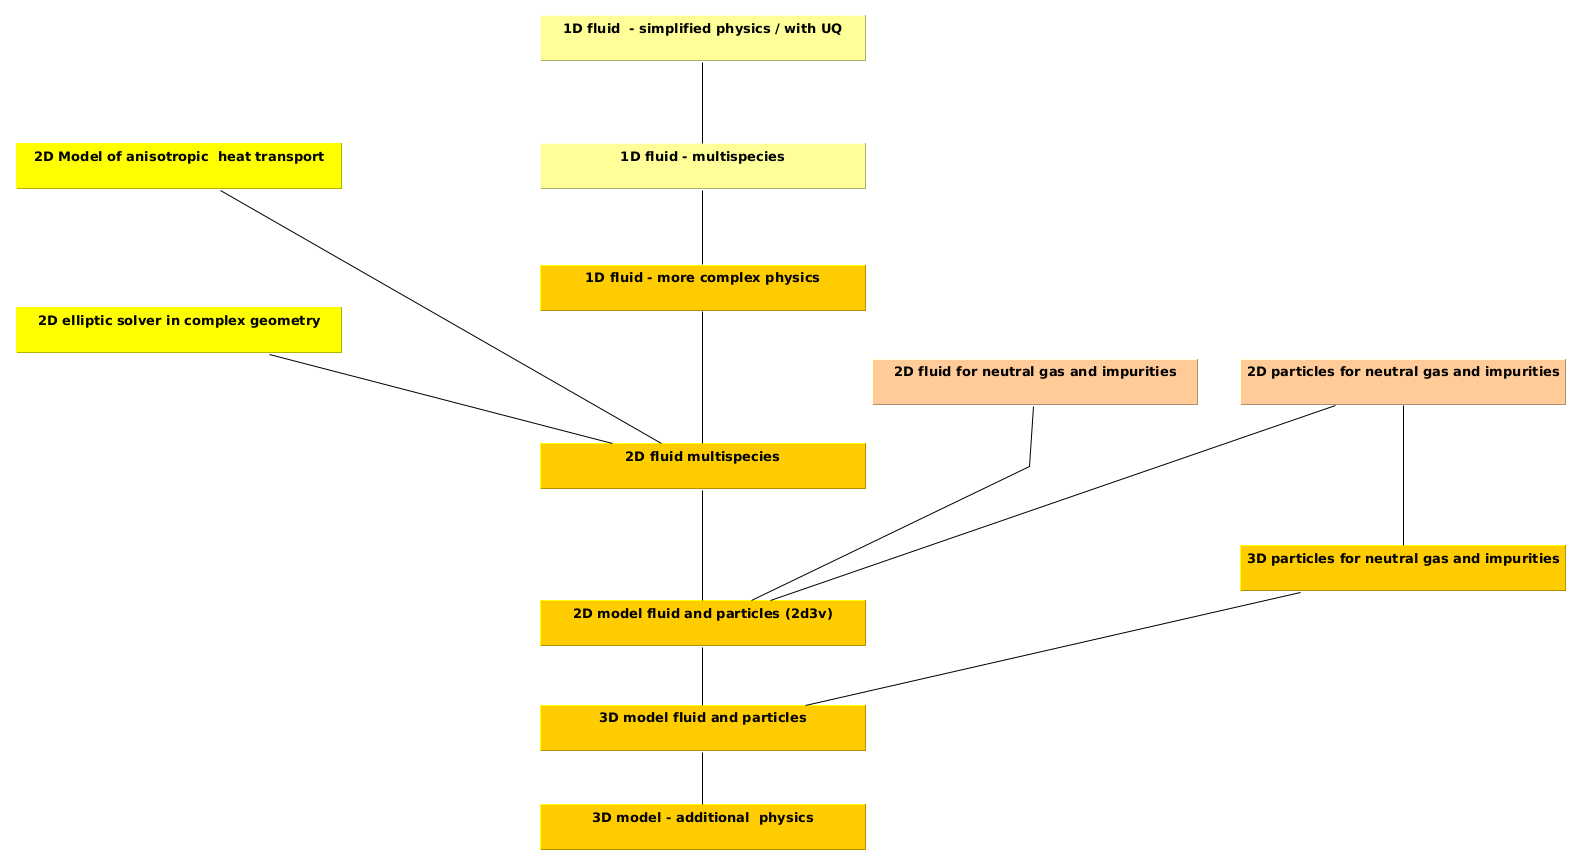
\includegraphics[width=0.95\textwidth]{./pics/proxyflow2.png}}
\caption{
Development of \nep \ software via a sequence of \papp s.
\label{fig:proxyflow2}}
\end{figure}

\subsubsection{Numerical efficiency}

``Numerical efficiency obtained for example through scalability to
large number of cores (given the expected computational resources, the
code should be designed to take: $\sim$1 week for low fidelity
parametric scans; $\lesssim$1 month for medium-high fidelity runs for
advanced design; $\lesssim$3 months for high fidelity physics studies).''

Order of magnitude estimates for the cost of code execution (see~\Sec{cg}),
indicate that these timings are possible but challenging.

The plan is to target Exascale simulations that can support high-fidelity physics
simulations.
Project \nep \ aims to do this in a performance portable fashion using abstraction
layers to separate the physics from the computation details.
However, the challenges of Exascale mean that a degree of
specialisation of the code towards available Exascale machines is expected.
At some point this will probably entail trade-offs that are detrimental to
performance on smaller machines.
Despite this, we still anticipate that the software
should be reasonably performant for small-scale runs.

\subsubsection{Stability of the code}

``Focus on stability of the code, using (preferably) unconditionally
stable numerical schemes and capability to diagnose and re-start failed runs.
Ensure a small failed simulation rate for common configurations.''

The focus will be on accuracy rather than stability.
An accurate solution will be a stable one, whereas the converse is not true.
The use of bifurcation tracking techniques is expected to help with numerical
stability. 
Moreover, the use of ensemble techniques (as part of uncertainty quantification)
should provide information on stability as a function of parameters, as well as
making it likely that at least a subset of calculations produces usable
results.

In addition, there are some planned technical solutions for diagnosing problems
with runs.
The simplest functionality is to allow users to change parameters when
restarting a job using checkpoint files.
The code can also be made to automatically check input files (to catch user
misspellings), and to output a file containing the parameters that were
actually used in a simulation (in case some were accidentally overwritten).
Simulations may also be given a Universally Unique Identifier (UUID) to allow
provenance tracking of simulations.


\subsubsection{Exhaust physics modelling capability}

``Provide capability to model exhaust physics all the way from sheath
limited to strongly detached regimes.''

This capability follows from (1) the implemented physics models/boundary
conditions, and (2) the lengthscales the code can resolve in simulations of
feasible run times.
Project \nep \ anticipates that this will be feasible. 
See \S\ref{sec:physics_model} for further details for the physical
models.


\subsubsection{Modern software design}

``Modern software design with modular approach (independent and efficient libraries).''

Project \nep \ is certainly adopting a modular approach to software design.
This is crucial for enabling many of the desired features, as noted below.
The use of reliable third-party libraries is also vital for enabling a small
team of developers to leverage the work of others, and to allow code
flexibility and ease of prototyping.

\subsubsection{Ability to integrate with other codes (eg.\ with IMAS).}
This feature is anticipated, and will be facilitated by writing the code in
object-oriented C++.

Integration with IMAS (and other data formats/standards) can be achieved by
writing a module to translate between \nep's internal data structures and IMAS
format.
\nep\ developers are involved in TSVV software which will also integrate with
IMAS, so will have experience in this area.

\subsubsection{Modern visualisation tools}
Integration with modern visualisation tools is not specifically addressed in
the science plan.
However, this is enabled by using standard data formats such as netCDF/HDF5.
Auxiliary tools (similar to BOUT++'s xBOUT library) could also be developed.

The issue of \emph{in situ} visualisation will also be important at the Exascale,
with the need to interrogate large quantities of data without moving it,
perhaps during a simulation.
Project \nep \ does not have specific plans for enabling this.
However, the need for this will be widespread, and we expect third-party
tools/libraries to become available to support this, particularly in C++.

\subsubsection{Accessibility (output easily catalogued and interrogated  big data)}
Given the constraint of producing Exascale volumes of data,
it is expected that \nep\ will default to using the Met Office practice of only
saving the files necessary for repeating a simulation, rather than full
outputs.
It is intended that key aspects will be captured by surrogates, descriptions of
which will be saved and indexed.
Users however will be able to choose to output more data and to define
custom diagnostics.
A modular approach to software design and the use of standard libraries will
ease the implementation of these.

In time, there will likely be a move towards creating
simulation databases in preference to repeating expensive simulations.
Such projects are nascent, but we have collaborators who are working in this
area.
Again, the modular approach and use of standard data structures will enable
interfacing with such databases as the technology matures.

% WA: It is expected that we shall adopt Met Office practice and only save the
% files needed to repeat simulations, rather than full outputs. It is intended
% that key aspects will be captured by surrogates, descriptions of which will
% be saved and indexed.
% JTP: Outputting more would be a user option though?

\subsubsection{Version control and user support.}
Version control is a fundamental part of modern software development, and will
certainly be used in \nep.
More generally, the project will use best software practices, including
protected branches, peer reviewed pull requests, issue trackers and automated
testing.
The main code contributors are familiar with such practices; we have heavy
involvement from the projects BOUT++ and Nektar++ which have very high quality
software practices.
Project \nep \ also have involvement from UKAEA RSEs.

User support will be provided through issue trackers, a project Slack or Zulip channel,
and where relevant, through training sessions.
Project \nep \ anticipates supporting several classes of user, from
those with limited software knowledge,
to users with appreciation of different numerical/algorithm choices,
through to numerical/software specialists who might edit the code on a granular
level.
Support for such a wide range of uses is enabled by a highly modular
separation-of-concerns approach.


\clearpage
\subsection{Physics model}
\label{sec:physics_model}

\subsubsection{General requirements}

\begin{quote}
``Equations need to be applicable to arbitrary aspect ratio devices.''
\end{quote}

The equations employed will not generically make the assumption of small
inverse aspect ratio.

\begin{quote}
The collision operators between plasma components, plasma and
impurities and plasma and neutrals have to be sufficiently accurate to properly
describe the radiation generated and the energy transfer between species.
\end{quote}

These operators may be included in the model being
derived in FM-WP2, but at this stage simpler model operators are being used.

\begin{quote}
``Photon opacity effects need to be included in the model.''
\end{quote}

The treatment of effects due to radiation are discussed in Annex~A of ref~\cite{pappeqs2}
(``the equations document"). Initial implementation will account only for
usage~(1) \emph{the calculation of source/loss terms}, with usage~(2) \emph{the production
of synthetic spectra}, depending very much on input from experimentalists,
as anticipated in the science plan~\cite[p\.\,11]{sciplan}.

\begin{quote}
``The equations need to be capable of dealing with multiple species in
non-trace amounts (at least D, T, He and seeding impurities).''
\end{quote}

The models being derived support distribution functions for multiple species.

\begin{quote}
``The equations should not rely on the Boussinesq approximation.''
\end{quote}

The model derived in FM-WP2 does not use the Boussinesq approximation.
Technically, this means \nep\ will need to be able to invert three-dimensional
elliptic operators with non-constant coefficients.
This capability will be available.

\begin{quote}
``The code should evolve both the electron and ion energy (temperature).''
\end{quote}
This is the case with the FM-WP2 model.

\begin{quote}
``It would be acceptable to have only axisymmetric equilibria,
potentially corrected through small perturbations.''
\end{quote}
This is answered by the discussion in \Sec{geometry}.


\subsubsection{High fidelity simulations}
\begin{quote}
``In high fidelity simulations, the kinetic/fluid transition for both plasma and
neutrals has to be properly captured, potentially using a multi-region approach
exploiting different models in different parts of the machine could be
considered (for both neutrals and plasma);
Boundary conditions need to consider improved sheath physics (collisional \&
shallow angles);
Ideally, the model should be able to treat de-magnetized ions in the divertor
region;
Electromagnetic effects should be included, but a perturbation approach would
be acceptable.''
\end{quote}

The Science Plan states that {\green ``FM-WP2 and FM-WP3 will concentrate upon
development of the two close coupled models of the \nep \  programme,
specifically FM-WP2 around the inclusion of kinetic effects into existing and
new edge plasma models, and FM-WP3 of particle based models for describing the
region outside and just inside the plasma (neutral atoms/molecules and
partially ionized impurities).''} See \Fig{colpri}.

\begin{figure}
\centerline{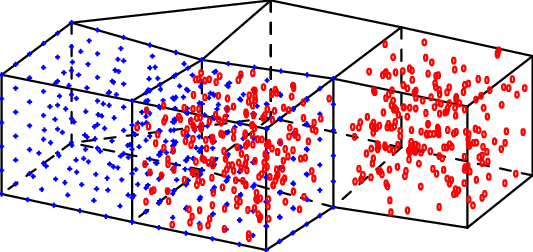
\includegraphics[width=0.7\textwidth]{./png/colpri.png}}
\caption{
\nep \ software will use finite elements and particles to represent different atomic species
as needed.
\label{fig:colpri}}
\end{figure}

In FM-WP2, a novel ``moment-based'' approach is being developed (for both
plasma species and neutrals).
This approach is a variant on gyrokinetics (though at present, the derivation
exists only for drift kinetics).
Instead of the stationary background Maxwellian of the usual gyrokinetics, this
approach uses a dynamically-varying background Maxwellian, where the
particle density, bulk velocity and temperatures are allowed to vary with time.
The result is a hybrid approach, where the software evolves both a fluid system
and a modified kinetic system.
One of the benefits of this approach is that it gives a natural means to
capture the fluid/kinetic transition, by switching between the fluid+kinetic
and fluid-only descriptions.
Moreover this approach allows the software to detect which of the fluid and kinetic
descriptions is valid in any region based on the properties of the modified
distribution function, and therefore to automatically evolve the relevant
model.

The favourable properties of this approach are valuable,
but as with any novel approach there is an inherent risk of the scheme not
working.  Thus as described in ref~\cite[\S\,1.1]{pappeqs2}, in the event that
this approach is not feasible, the kinetic calculations
will use a Particle-in-Cell (PIC) approach.
While full orbit PIC is potentially extremely expensive relative to gyrokinetics,
it has been very well-studied both in terms of theory and numerical implementation.
Moreover the issue of how to treat the transition from fluid to a particles in
a coupled model is well-understood, at least in classical fluid dynamics.

Relevant sheath physics boundary conditions are being derived as part of this
work, including shallow angles and collisions.
Ions which exit the domain re-enter as neutrals with the Knudsen cosine
distribution.

While the current derivation is electrostatic, there is nothing which precludes
the derivation of an electromagnetic model.


\subsubsection{Neutrals and impurities}

\paragraph{Different levels of multispecies capabilities should be considered.}
The framework nature of the code means this will be the case.

\paragraph{In medium to high fidelity models, neutrals and heavy species should
be treated fully kinetically (the former have potentially low collisionality
and they are not bound by the magnetic field, the latter have a large Larmor
radius).}

Development of a neutral gas and impurity model is ongoing under FM-WP3. 
Page 7 of the Science Plan states: {\green ``Kinetic levels of complexity are \ldots
necessary \ldots for modelling the burning plasma regime, due to the inherent
uncertainty in the fluid codes. 
The plasma in a fusion reactor may well behave significantly differently to
plasma in existing devices because it will in general contain two main ionic
species (Deuterium and Tritium), neutral fuel particles and ionised Helium ash
(or alpha particles), as well as impurity ions originating from the wall.''}
That is, kinetic models will be derived and implemented, though it is hoped
that this will facilitate the development of fluid models.

\paragraph{In high fidelity models, dynamical neutral evolution on the
turbulence time scale would be preferable, if possible.}
High-fidelity simulations will use a kinetic model for neutrals where appropriate. 

\paragraph{Ability to model pumps (either directly or via pumping surfaces)
should be included. Pellets: the code should enable simulation of, or coupling
to models that can model, pellet fuelling.}
Models for these aspects are not included in the Science Plan.
As we will use an unstructured mesh, it will be possible to describe arbitrary
pumping surfaces.

The role of sources and sinks is recognised to be crucial in \nep\ physics so
that modelling of pellets as a source will be possible.
The tool CWIPI (Coupling With Interpolation Parallel Interface) may be used for
coupling to more complicated pellet models.

\clearpage
\subsection{Physics capabilities}
\label{sec:physics_capabilities}

``The code needs to be able to give reliable predictions of:
\begin{itemize}
\item[$\bullet$] Divertor loads:
\begin{itemize}
\item[$\bullet$] Reliable calculation of upstream particle and heat flux
	profiles: proper drift physics and upstream turbulence;
\item[$\bullet$] Divertor turbulence: turbulence spreading in the divertor
	region, effect of magnetic shear next to the X-point(s) to understand
	upstream/downstream connection;
\item[$\bullet$] Multifluid capacity to model radiation and detachment physics;
\item[$\bullet$] Reliable calculation of the electric field (collisionless
	physics near the separatrix, proper reflection of neutrals at the
	target);
\item[$\bullet$] Able to capture in/out and top/down asymmetries (geometry,
	drifts, radiation and detachment)
\end{itemize}
\item[$\bullet$] Wall loads:
\begin{itemize}
\item[$\bullet$] Should be able to predict filamentary transport and role of
	hot ion confinement (wall erosion)
\item[$\bullet$] Should calculate radiation and neutral loads (may require
	dedicated modules, same for divertor loads);
\end{itemize}
\item[$\bullet$] Impurity transport, pumping and fueling:
\begin{itemize}
\item[$\bullet$] Ability to track low (He Be), medium (C, N, Ne) and high Z
	impurities (W, Ar, Xe) with multiple charge states;
\item[$\bullet$] Reliable kinetic modelling of neutrals to assess fueling and
	pumping capacity;
\item[$\bullet$] Ability to handle non-trace species (D, T, He, seeded
	species), which requires new closures for the equations (if fluid,
	beyond Braginskii $\implies$ Zhdanov or better);
\item[$\bullet$] Accurate model of friction forces (turbulence + neoclassical
	on open field lines);
\item[$\bullet$] In high fidelity models, the code should be able to simulate
	localized gas puffs, via injection of neutral particles.
\item[$\bullet$] Dust  the code should enable coupling to codes to simulate
	dust generation, transport and ablation, via exchange of fluxes and
	sources.''
\end{itemize}
\end{itemize}



\paragraph{Physics models.}
Many points in this section relate to the physics model.
As we have alluded to above, the actual physics model used is the
responsibility of the user;
so, for example, it will necessary for users to derive an accurate model for
turbulent friction.
Moreover, as \nep\ will initially be an edge code, only electromagnetic
radiation from the edge plasma will be calculated, and an additional model will
be required for radiation for the core plasma. 
%{\blue Is that what is meant about radiation?}
Nonetheless, we plan to facilitate models which have the listed properties.
In particular, our meshing approach will allow accurate representation of the
walls and divertor.
Thus powerful and flexible source/sink models may be used, for both volumes and
surfaces.

\nep\ code will also be capable of representing scales on which filamentary
transport has been calculated to occur.
The code will only produce fluxes however, and it will be up to the user to
calculate wall erosion.



\paragraph{Validation, Verification and Uncertainty Quantification (VVUQ).}
Naturally, when the solution of a problem is unknown, it is difficult to assess
whether the provided answer is reliable as requested in the first line of the current section.
Therefore we are integrating \nep\ with a suite of tools for VVUQ to enable
validation of code outputs against experimental results, and provide a error
bars for code outputs due to the uncertainty in the code inputs.
As allowed by error estimates, models of different complexity will be used
to predict key properties of the SOL, see \Fig{dimensions2}.
\begin{figure}
\centerline{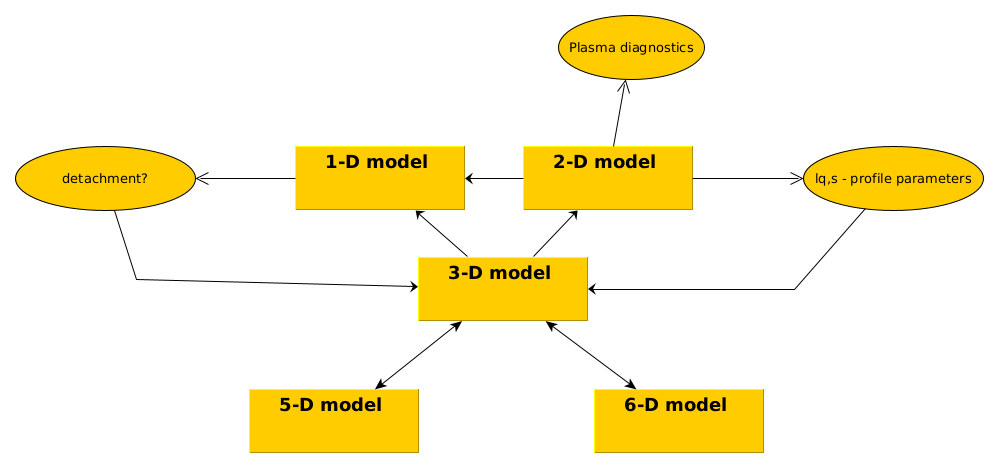
\includegraphics[width=0.7\textwidth]{./pics/dimensions2.png}}
\caption{
Project software will integrate a range of models of different complexity, here
indicated by their dimensionality.
\label{fig:dimensions2}}
\end{figure}

\clearpage
\subsection{Geometry}\label{sec:geometry}

\begin{quote}
``Ability to handle complex topologies and novel geometries:
\begin{itemize}
\item Capacity to treat different topologies with multiple X-points ($>$2),
	possibly in a dynamic way, or at least implemented in a way that does
	not preclude time-varying equilibria being modelled in future; 
\item Ability to handle singularities in the grid (null points) or to develop
	accurate scheme(s) that do not have singularities;
\item Ability to interface with 3D CAD designs of the machine; 
\item Capability to handle conformal grids that go all the way to the wall for
	both neutrals and plasma; 
\item Capability to treat subdivertor structures (only neutrals).''
\end{itemize}
\end{quote}

\nep\ will use a spectral/hp finite element approach.
This allows considerable flexibility in meshing, with elemental tetrahedra,
hexahedra or prisms being used to describe complex geometries.
In addition to refinement of the elemental grid sizes ($h$-adaptivity),
the order of the piecewise polynomial basis functions used on each element may
also be changed ($p$-adaptivity).
The production of finite element griddings conforming to CAD descriptions is standard
for virtually all meshing packages. Project \nep \ will specially aim to use
the small number of packages that may produce finite elements with curved edges and faces 
to exploit fully the higher order basis.
This gives a framework which can achieve spectral convergence on complicated, conforming grids,
while still being able to handle discontinuities in the solution.

%Unlike approaches based on deformations of Cartesian grids
%{\blue (JTP: is this what is meant by conformal mappings here?)},
Should it prove necessary to produce a meshing conforming to
surfaces of an equilibrium magnetic field, then because
the finite element approach does not require a structured grid, it should
be able to treat arbitrary geometries and topologies, 
in particular including multiple X-points.
The approach could be extended by further use of adaptive meshing to allow for time-varying equilibria.

%From the science plan
%\begin{quote}
%	``[NEPTUNE] work will initially focus upon coupling the turbulent plasma periphery
%	to the surrounding neutral gas and partially ionized impurities that
%	exist between the plasma and plasma facing components, in the presence
%	of an arbitrary tokamak magnetic field and full 3-D first wall
%	geometry.''
%
%	``Infrastructure and workflows will be developed so that the resulting
%	close coupled models can be constructed routinely based around a
%	high-fidelity representation of the geometry described by Computer
%	Aided Design (CAD) systems (this likely requiring the development of
%	high order meshing technology, e.g.\ using Nektar++).''
%
%	``P4. Accurate representation of first wall geometry (face normals to
%	within 0.1$^\circ$), and correspondingly of complex magnetic field
%	geometries.''
%
%	Solvers in complex geometries part of ``Plasma multiphysics model
%	(Fusion modelling, work package FM-WP2)''
%
%\end{quote}

\begin{subappendices}
\warpprintonly { \section{Order-of-magnitude estimates for tokamak edge modelling}  \label{sec:cg} } 
\warpHTMLonly{ \ForceHTMLPage \refstepcounter{section} \section*{Order-of-magnitude estimates for tokamak edge modelling} \label{sec:cg} \phantomsection \addcontentsline{toc}{section}{[\getcurrentref{chapter}.A] Order-of-magnitude estimates for tokamak edge modelling} 
}

Suppose plasma number density $n \approx 10^{18}$\, m$^{-3}$. Order of magnitude
dimensions are $L\approx0.1$\,m for SOL thickness, reactor minor and major radii
say $a=3$\,m and $R_0=10$\,m, so the volume of SOL $\approx 4 \pi^2 a R_0 L \approx 100$\,m$^3$.
It follows that the total number of electrons $\approx 10^{20}$.

The shortest timescale is inverse $e B/m_e$, the electron cyclotron frequency, where the
ratio of charge to mass for the electron is
$|e|/m_e = 1.76 \times 10^{11}$\,C kg$^{-1}$, and $B\approx 10$\,T, so $\tau_{Be}\approx 10^{-12}$\,s.
Hence the number of particle-steps to evolve $1$\,s of physical time is  $10^{20+12+1}$
(assuming of order $10\pi$~timesteps per orbit),
which assuming $1000$\,flop per update, needs a total of~$10^{36}$\,flop.
Thus to complete a computation in $1$\,s on Exascale machine, only one
$1$~particle-step in $10^{18}$ is allowed.
This implies for example only $100$~superparticles in the volume can be used supposing
each has a weight~$10^{18}$, which
is unlikely to be adequate because electrostatic and other effects will produce a noise level
that swamps any physical effects. However if $3$ or $4$~months (approx.~$10^7$\,s) are allowed, then
a calculation with~$10^9$ particles may be performed if memory-access bandwidth constraints
can be satisfied, when the noise levels may be manageable.

The situation may be shown to be a million times easier for neutrals considered
separately, assuming neutral density~$n_0=n$, particle mass~$m_p$ and temperature~$T_0=10$\,eV, for a
timescale of~$\tau_{0}=L_{mfp}/v_0$ where the mean free path~$L_{mfp}\approx L$ and the neutral
speed typically is~$v_0$. For then $v_0=\sqrt{|e|T_0/m_p}
=\sqrt{|e|/m_e} \cdot \sqrt{m_e/m_p} \sqrt{T_0}$, ie.\ 
$v_{0}\approx 4 \times 10^5 \times (1/40) \times \sqrt{10}\approx 3 \times 10^4$. Thus
$\tau_0\approx 10^{-6}$\,s, ie.\  a million times longer than the electron cyclotron timescale.

Suppose a fluid model is employed instead, ie.\ the electron distribution is
represented by its first~$3$ moments.
If the electron temperature~$T_e \approx 10$\,eV, then the
thermal speed $V_{Te}\approx 40 v_0 \approx 10^6$\,m s$^{-1}$. Supposing the SOL to be sampled at a
uniform~$1$\,mm interval, then the
number of sample-points~$\approx 10^{11}$, and the timestep for an explicit scheme~$\approx (10^{-3} /10^6)\approx 10^{-9}$\,s,
so the number of sample-point updates is $10^{11+9}$. Assuming  $1000$\,flop each update, this
means one second of physical time needs $10^{23}$\,flop or $10^5$\,s$\approx 1$\,d
of Exascale machine time, if memory-access bandwidth constraints can be satisfied. If an implicit scheme
is used to simulate plasma ions as a fluid on a drift type timescale$\approx L/V_{Ti}$, then
possibly the timestep~$\tau_i\approx \tau_0\approx 10^{-6}$\,s, ie.\ a thousand times larger, and
calculations lasting only a few minutes might suffice.

Another way of looking at this is to suppose that numerical problem is $D$-dimensional, $1000$\,flop
are needed for each sample update
and $N_D$~samples per spatial dimension and $N_D^2$ time samples are allowed. Then to update
such a model in $1$\,s requires
$N_D^{D+2} \approx 10^{15}$. Thus  if $D=3$, $N_3 \approx 1\,000$, and $N_5 \approx 100$.
It seems that accuracy controlled, unstructured, implicit fluid models should be possible,
although for the more complex models $1000$\,flop per update may be an underestimate by
orders of magnitude.


\end{subappendices}

\newsection{Software Engineering Response}{sec:TS_sw_response}
The above scientific response~\Sec{response_physics}  indicates that the \nep \ suite
will have the capability to describe the tokamak edge in a 
comprehensive set of levels of detail using a large range of possibly 
heterogeneous computer hardware, will be straightforwardly modifiable to 
include additional physical effects, and will aim to include under all 
circumstances, the level of error in computed results.
Evidently, eveloping the suite represents a major challenge to current software engineering
practices thanks to its scientific difficulty as indicated in \Sec{cg},
and perhaps less obviously, its scientific \emph{complexity} due to the need to treat
large numbers of atomic and molecular species, descending to the level of isotopes
with a range of charge states and electronic excitations.

The last  makes \nep \ a  significantly harder development than the BOUT++ code
discussed in \Sec{response_physics}. The difficulty motivated studies of software
engineering practices outside as well as in the scientific context.
The studies of scientific work are summarised in reports  concerning frameworks,
scientific UQ etc. Ideas from these studies are combined with non-technical works
such as Hewitt~\cite{hewitt} and Sommerville~\cite{sommerville} and
summarised in the report~\cite{y2d34}. 

The outcome is the present report and website, which augment the procedures of
Dudson and BOUT++ collaborators~\cite{y3re314}  to govern the development of \nep.
Management aspects of the development are treated in \Sec{MGT_intro} and
operational aspects in \Sec{OP_MGT}. The remainder of this section focusses
on the generic details of a software implementation, the so-called
non-functional aspects,  with BOUT++ instructions
augmented to allow for the greater complexity of \nep, following the D3.3
reports~\cite{y2d33}, here with~\Sec{TS_varnames} adding a way to handle a multitude of variable
names to accommodate the much increased number of physical variables.
%Conventions
%Latest C++, C++20 if/when possible including modules (like Fortran-95 only import instead of use), and
%concepts - generalised types of single variable.
%Follow Stroustrop~\cite{stroustroptour}, also
%C++ Core Guidelines (Bjarne Stroustrup, Herb Sutter)
%\url{https://github.com/isocpp/CppCoreGuidelines/blob/master/CppCoreGuidelines.md}
%Philosophy section can be condensed to
%\begin{itemize}
%\item Know, and use, available libraries, particularly the Standard Library and the Guideline Support Library.
%\item Also, know, and use, available language features.
%\item Use language to ensure that the purpose of code is unambiguous.
%\item Consider writing a library if none is already available (and presumably making it available to others).
%\end{itemize}

%Use of clang\_tidy, on source code, enforce pot-hole convention.

%Reject unapproved packages

%Two options maintained

%Prepare documents so easy to generate 5-15 slide presentations

%Functionality, expected performance/accuracy, external interface %Smith

Following D3.3~\cite{y2d33}, \Sec{TS_considers} discusses high-level constraints on the structure of software.
where the concept of division into packages and modules (which may represent libraries)  is promoted.
\Sec{TS_scistruct} explores the implications of these constraints for \nep.
At the opposite extreme to \Sec{TS_considers} and \Sec{TS_scistruct},
\Sec{TS_lowlevel} describes the desirable contents for a single module,
and \Sec{TS_procio} discusses the question of what best to output when developing 
software for the Exascale.

\subsection{General Considerations}\label{sec:TS_considers}
It is important that individual units of code are manageable and the overall
structure is comprehensible, so that developers and users can navigate the codebase
and determine where new work is to be located.  This simple consideration implies
that \nep\ software should be divided into units that it will be convenient to refer
to as modules, ie.\ sections of code containing everything necessary to perform one
(and only one) aspect of the desired functionality.

The suggested content of a module
describing a single class in the UML sense (see \Sec{TS_lowlevel}, \Tab{TS_umltrans})
implies a minimum of $13$~methods described by separate subroutines/functions,
with examples extending up to $50$, although the latter is there regarded as an excessively large
number of methods.
Many small software libraries also fall into this size range.
Supposing that each subroutine is of a length to fit within one computer window, ie.\
up to about~$60$~lines, the desirable maximum length of a well-designed module file is
$30\times60 = 1\,800$~lines which is a manageable size of file given 
editing software that remembers on restart, the last line accessed (so that it possible
to return immediately to a particular subroutine).
The magnitude of the D3.3 exercise follows from
the fact that comparable software packages probably of somewhat lesser complexity
than \nep\ written in high level languages such as C++ range in size up to~$1\,000\,000$ lines.
Clearly $400$~separate modules is too unwieldy, and there is a need to organise
further into packages which might contain in turn $10$-$50$ modules. 
As a way of providing further indication to developers,
it is helpful to talk of packages as being arranged into layers, as discussed
in~\cite[\S\S\,2.4,3.2]{y2re333}, see \Fig{hierarchygroup}.
Then, as prefigured in~\cite[Annex~A]{y2re333}, it should be  possible to encapsulate
the necessary complexity in one, albeit large diagram.
\begin{figure}
\centerline{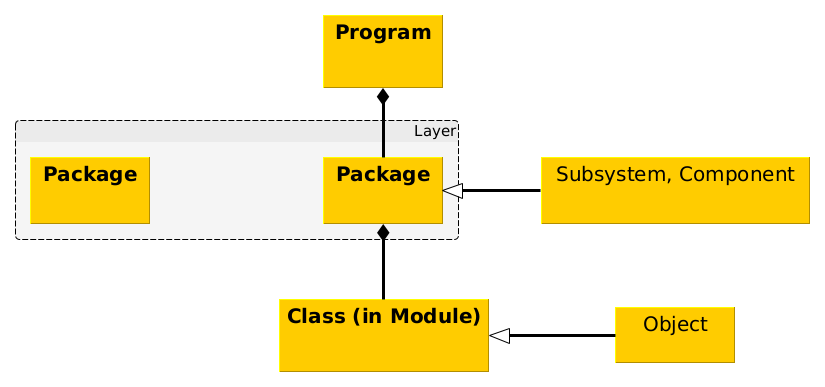
\includegraphics[width=0.7\textwidth]{./png/hierarchygroup.png}}
\caption{
Sketch of relationship between units of large code.
\label{fig:hierarchygroup}}
\end{figure}

\subsection{Considerations for Scientific Software}\label{sec:TS_scistruct}
\subsubsection{Structural Considerations}\label{sec:TS_structure}
In both~\cite{y1re331,y2re332}, a figure from Dubey~et~al~\cite{Du16Idea} is reproduced
that illustrates how scientific software may be developed by beginning with an ``infrastructure"
capability into which initially exploratory scientific software is integrated as its worth
is established. Unfortunately for \nep, it is not clear initially what  aspects  of the infrastructure
will be durable and stable, although once the software is more mature, Dubey~et~al's methodology
appears attractive.

The literature referenced in~\cite{y2re333}
indicates that scientific software should be produced by aggregation, but is less
helpful as to what is to be aggregated, ie.\  the modular decomposition as to what should
constitute a single module etc.
%Surprisingly little detailed discussion was found in the literature
%after the early book by Booch~\cite{booch}, as to how to create classes in
%the scientific and engineering context, with the exception of Douglass~\cite[\S\,5]{douglass}.
%The ideal would be a way to create classes that enabled rapid development  of code
%that executed efficiently but was easily re-used.
%%where flexibility is also an important consideration,
%Douglass~\cite[\S\,5]{douglass} does not specifically address these last points, but they
%could guide choice of objects in his approach which is reproduced as Appendix~\Sec{TS_objdisc}.

Since the \nep\ development will proceed as a series of \papp s, there is a chance
to refine and redefine an initial modular decomposition with each successive \papp,
recording the results as a UML structure diagram. When generating the corresponding
sequence diagram (ie.\  procedural description), the \papp-based units should be preserved to
facilitate the use of the simpler ones as surrogates for the later more complex \papp s.

To help understand the  aggregation of the software, it should be layered in the obvious manner,
with the higher layers corresponding to greater numbers of aggregated objects. It is also expected
to be useful to classify the modules.
The modules should be arranged into a relatively small number of packages according to, 
eg.\ whether they treat particle generation, matrix coefficient calculation, the main matrix solution, or visualisation.
%\clearpage
\subsubsection{Interactions between Modules}\label{sec:TS_modulint}
Concerning logical interconnections between modules, the 
use of  a directed, acyclic graph~(DAG) structure might be thought mandatory,
particularly to  process the input
data in order to specify coherently the construction of the elements of the solution matrix.
However, as prefigured in~\cite{y2re333} for the gyrokinetics code \F{GS2},
the tightly coupled nature of the central edge
physics problem  means that input is more about gathering \emph{all} the data, for only at that point
can fields be computed and only after that may matrix coefficients be computed.

(TODO) ``Information hiding principle" eg.\ input data module ``hides" information about how this is done from
the calculation module: it just passes along parameters in an agreed format.
Can extend this idea on to every level - eg.\ Parnas advocates hiding the hardware from the code -
cf.\  performance portability.
Such modularity  enables work to be efficiently  assigned to a programmer or group.

\subsection{Design of a Module}\label{sec:TS_lowlevel}
\subsubsection{Notation}

%It should be noted that when discussing software in text documents,
%the following conventions in \LaTeX\  are used
%\begin{itemize}
%\item \F{Small capitals} denote a package name
%\item \I{Italics} denote a program name
%\item \T{Fixed width font} denotes any code name or fragment which is not otherwise obviously source code
%\item \B{Bold} denotes a shell script name
%\end{itemize}
%However special fonts are not employed if the class is identified by a
%suitable suffix, thus ``\_m" for a module containing executable code defining methods,
%``\_h" or ``.h" for class attributes (equivalently derived type or namespace code), ``.cpp" for name of file containing 
%C++ source, ``.exe" for an executable, etc.
%Note that Object Fortran has led the way in that 
%requires only one copy of a class's attributes to be compiled, whereas only the very latest versions of C++
%avoid recompilation of namespaces when a .cpp file is changed.
UML nomenclature is preferred herein, for which \Tab{TS_umltrans} provides a limited 
translation into C++ and Object Fortran. % is reproduced as Table~1 in~\cite{y2re332}.

\begin{table}[tbph]
\begin{center}
\caption{UML interpreted as Object Fortran and C++ \label{tab:TS_umltrans}}
\begin{tabular}{|p{5cm}|p{5cm}|p{5cm}|}
\hline
UML & Fortran 2003 & C++  \\
\hline
Class & Derived type & Class \\
Part  &  - & Component  \\
Attribute & Component & Data member \\
Method & Type-bound procedure & Virtual Member function \\
Feature  & Component and Type-bound procedure & Data and Virtual Member function \\
Structured class & Extended type & Subclass  \\
Specialisation & Class & Dynamic Polymorphism \\
Generalisation & Generic interface & Function overloading \\
\hline
\end{tabular}
Further insight into UML terminology may be gained from the description
of the patterns in~\cite{y2re332,y2re333}.
\end{center}
\end{table}


\subsubsection{Module design}

The focus herein is the structure within a module. Specifically, the module describes a single class or object
(strictly speaking in UML terms, objects are instances of a class), which is
fundamental in that it is defined without use of aggregation.
The software  - consistent with Clerman and Spector~\cite[\S\,11]{clermanspector} -
that is promoted by Arter et al~\cite{fprog} for an object-oriented language, recognises two sizes of fundamental class
and it is easier to start by considering the smaller, denoted smallobj\_m.

Module smallobj\_m does not have a separate attributes file, but will typically still use or access
three or more yet more fundamental classes, namely
\begin{itemize}
\item log\_m for logging errors or warnings in code execution, and checkpointing values of selected variables
\item const\_numphys\_h for numerical values of important mathematical and physical constants relevant to plasma physics
\item const\_kind\_m to specify precision of representation of real and integer values, together 
with formatting to be used for their output (in fact contains no executable code)
\item date\_time\_m to return the date and time in either a verbose or minimal format
\item misc\_m to form miscellaneous operations found to be common to many modules
\end{itemize}
In outline, the  methods or operations associated with \T{smallobj} allow data to be read from a named file,
used in the construction of an object, and output to disc file. The file is given a numeric identifier~\T{ninso}
(file~unit) when it is opened. Data used to construct the  object forms a single \T{namelist} block, viz.\ 
a list of arbitrary code variables that may (or not) be assigned values in the input file using a attribute-value notation.
Namelist variables should have long names that promote a good user interface, and
be given default values in case they are not input.
The style encourages checking that inputs have acceptable values, for example lie in expected ranges,
but there is no equivalent of eg.\ the Cerberus Python data validation package~\cite{cerberuswebsite},
users must explicitly code checks and calls
to log\_m if the values are questionable or erroneous. (It is hoped that this can be automated based
on a \LaTeX \ table describing input symbols. After successful checks, the values in
the namelist are copied into the data type sonumerics\_t, whence it is supposed that a single subroutine then
instantiates the smallobj\_t object. Another routine performs
output of this object, either to a directly specified file unit, or
to the standard output by default, in the simple text format of a variable name followed by its value on the following
line. As might be expected, there are also routines to `delete' the object, ie.\ to deallocate
any constituent arrays, and to close the input file.
The precise list of member functions (or methods in the UML nomenclature) is
\begin{itemize}
\item initfile,  open input file
\item readcon,  read data from input file
\item generic,  generic subroutine to instantiate object
\item write, write out object to standard output, or to file opened by another object
\item delete, delete object
\item close, close input file
\end{itemize}

Module bigobj\_m has a separate file for its attributes (\emph{aka} namespace), which it will
normally still use or access
like the yet more fundamental objects listed for smallobj\_m. However the data types
defined in bigobj\_h are of the same kind as those in smallobj\_m, viz.\ bonumerics\_t
to hold input data which is used to define bigobj\_t by calling the \T{solve} subroutine
(rather than the subroutine \T{generic} in the case of smallobj\_m). Apart from
this last  exception, the methods in bigobj\_m are a superset of those in smallobj\_m.
The additional methods recognise that instantiation may involve
more than one routine and in particular may involve use of a specially defined
function \T{fn}, demonstrating the STRATEGY Pattern or possibly TEMPLATE Pattern.
This function may be determined by a formula identified in the input,
giving  the option for a developer or determined user of adding their own code to define
a new function. The range of allowable outputs is much extended. Thus there
is a separate routine provided for output to the log file using what will
probably be a lengthy list of calls to log\_value\_m. More likely to be useful  is a routine
to open an .out file on a file unit given the number~\T{noutbo} on opening, which
becomes the default unit for writing out the object in \T{bigobj\_write}.
There are also provided separate skeleton routines intended to provide output
in a format suitable respectively for visualisation by \F{gnuplot} and \F{ParaView},
and of course routines to close files and delete the object.
The precise list of member functions for bigobj\_m is as follows
where those also found in smallobj\_m are enclosed in parenthesis:
\begin{itemize}
\item (initfile),  open input file
\item (readcon),  read data from input file
\item solve,  generic subroutine to manage instantiation of object
\item userdefined,  user-defined method or function
\item fn, general external function call
\item dia, write object diagnostics to log file
\item initwrite, open new file, making up name which defaults to having .out suffix
\item (write), write out object to standard output, or to file opened by \T{bigobj}
\item writeg, write out object suitable for  visualisation by \F{gnuplot}
\item writev, write out object suitable for  visualisation by \F{ParaView} 
\item (delete), delete object
\item (close), close input file
\item closewrite,  close write file opened by \T{initwrite}
\end{itemize}

Thus the skeleton object is defined by a formula plus data input from disc,
and since both are saved internally as features, the instantiation may be deferred as necessary,
so-called `lazy initialisation'.
It will be noticed that other variables in bigobj\_m such as unit number are hidden, ie.\ cannot be accessed by
other modules. In fact a common addition to the default modules is a method function \T{getunit} that returns \T{ninbo},
illustrating the approved way of accessing such data.

%The source as mentioned in~\cite{y2re333} may be obtained by download of
%program~\I{smardda-qprog}~\cite{qprogwebsite}.
The reason for the emphasis on input and output from and to disc (I/O)
is to facilitate the construction of a test harness
for an objects in the style of bigobj\_m, and indeed the aggregations of such objects.  
The use of ``attribute-value" in I/O gives flexibility to the developer, since new variables may be
added without the need to modify existing input files or output processing. Output processing is further
discussed in \Sec{TS_procio}.

%In the course of a software development, the source code relating to an object naturally grows
%with the addition of further subroutines in the module file.
%Since \nep\ is anyway going to have to describe the equilibrium magnetic field~${\mathbf B}$ it
%is worth examining what such growth led to the beq\_m \F{SMARDDA} module
%besides the standard routines listed above.
%In fact beq\_m grew to $50$~routines (the number probably indicating a need for refactoring) so they will
%not be listed in full. $13$ of the new routines are concerned with either reading or writing from disc,
%reflecting the ability to handle a range of formats of the so-called `eqdsk'~type, plus an ability
%to define the magnetic field analytically. The eqdsk and analytic description assume axisymmetry
%with the field defined by the magnetic flux function~$\psi(R,Z)$ where $(R,Z)$ are cylindrical polar coordinates
%centred on device major axis. Much of the module complexity is accounted for by the needs either to verify
%that the field has been correctly read in as the `eqdsk' format is not standardised, or
%to return ${\mathbf B}$ in either flux, polar or Cartesian coordinates,  in formats avoiding storage on
%a whole~$360^o$ mesh. Onto this structure
%was subsequently bolted capabilities to superimpose a non-axisymmetric vacuum field (which is not strictly an
%equilibrium field) and to track through the $\psi$-landscape for various purposes.
%
%Representative routines in beq\_m are
%\begin{itemize}
%\item fixorigin, which fixes a problem encountered when the data in
%the eqdsk extends to $R=0$ because eg.\ the $Z-$component of ${\mathbf B}$ is defined as $(1/R) \partial\psi/ \partial R$.
%\item sense, which returns the sense of helicity of the field
%\item psilt, to calculate the actual range of values of $\psi$ by resolving possibly conflicting inputs
%\item ctrackc, return the track in~$(R,Z)$ running through the plasma centre of the extremum of $\psi$
%\item init, which initialises the field, the equivalent of \I{solve} and/or \I{generic}
%\end{itemize}
%Arguably $\psi$ should be disaggregated as a separate class for the purposes
%of tracking extrema etc. In one sense, it is already separate because  it constitutes a
%2-D spline class, being of type spl2d\_t defined in modules spl2\_m. 
%However the latter is conceptually a mathematical construct, whereas the analyses in beq\_m are
%physically conceived, which is why they were placed there. This illustrates one of the difficult dilemmas
%that may arise from the object-oriented approach in scientific applications. Another feature
%of scientific work is the use of simple analytic formulae either for testing purposes 
%or to include an effect such as field ripple to get a qualitative feel for its influence,
%rather than always using detailed machine data to get a full quantitative evaluation.


\subsection{Processing Module Output}\label{sec:TS_procio}
The number of I/O subroutines can be criticised.
For many testing purposes an interactive debugger is adequate,
and for most others that one output file is sufficient provided it is in a attribute-value
format such as JavaScript Object Notation~(JSON) or in a self-documenting format such as the 
Network Common Data Form~(netCDF), to be interpreted by any suitable visualisation software.

The problem with scientific software, worse
at Exascale, is the volume of data to be handled so that the ability to visualise large arrays
as well as large numbers of small arrays is essential (no debugger as far as is known has 
such a visualisation feature).  Moreover, the actionable aspect of \nep\ further means
that any postprocessing of a generic file must also be carefully performed. Thus while
a generic output file could be processed by say Linux \T{awk} script into a form suitable for
\F{gnuplot} processing, this gives rise to a need for providing documentation and
provenance for the script, which is at minimum a nuisance. Worse is the risk that the amount of
data to be processed may be so large as to lead to significant
delay and maybe even system or other issues not handled well if at all by the script, all of which
may be extremely time-consuming to resolve. Other conversion software may not be available
or properly implemented on the target machine.
Thus even for debugging purposes, it seems desirable that as much as possible of the processing
is done within the main code, and for production runs, output in a format
directly readable by say~\F{ParaView} should also speed the post-processing.
Since netCDF may be read directly by~\F{ParaView}, this is recommended.




%\section{Technical Specification}\label{sec:TS_MGT}

\subsection{Code licence and availability} \label{sec:lic}

Code should be made available to collaborators at the earliest opportunity, to maintain
close alignment between groups. 

\begin{itemize}
\item To minimise friction and unnecessary legal restrictions on combining
code components, a common, MIT licence has been adopted. This may be regarded 
as equivalent to the BSD3 licence in the \nep \ Charter, see~\Sec{charter}.

\item
Code development should be carried out in public
repositories. The benefits of minimising delay to code use, feedback
and peer review, outweigh any potential for embarrassment or code misuse.
\end{itemize}

\subsection{Code style} \label{sec:style}

There are many different code styles, each of which have their
proponents, and can be debated at length.  While everyone has their
own favourite style, it seems likely that the choice of style makes little
difference to objective quality or productivity.  Anecdotal experience
and experience from the gaming world in developing large, complicated packages
(eg.\ Gregory~\cite[\S\,3]{gregory}),
indicate however that it is very important that there is a well-defined
code style and that developers stick to it, since a mixture of
styles in a code base adds unnecessary mental load and overhead.
The ultimate choice is down to the project Lead, under advice from
major code contributors, leading websites and textbooks, eg.\ in the
case of the C++ language, the C++ core guidelines~\cite{cppguidelines}
and more compactly Stroustrop's ``Tour of of C++"~\cite{stroustroptour}.
 
The following style choices have been made and efforts will be made to enforce them
in \nep \ repositories.
\begin{enumerate}
\item Formatting of C++ and Python will follow the style used by Nektar++
\begin{itemize}
\item Developer tools: Code formatting tools should be used to
automatically format code.  For C++ \T{clang-tidy}~\cite{clang-tidywebsite}
should  be used while, and for Python \T{Black}~\cite{blackwebsite}
is recommended. Similar tools should be chosen
for any other languages adopted by the project.

\item Enforcement: Tests run on pull requests and code pushes to the
shared repository should include code formatting: The automated
formatter is applied to the code, and if the output is different
from the input then the code is incorrectly formatted, and the test
fails.

\item Documentation: \LaTeX \ or Markdown should be used
and conventions enforced regarding a maximum line length of $120$~characters,
restriction to ASCII character set, abbreviations, hyphenation,
capitalisation, minimal use of~`z', and use of fonts to denote code names.
The \LaTeX \ {\tt lwarp} package is used to generate this website.

\end{itemize}

\item Naming 

Naming of code components (modules, classes, functions, variables
etc.) is less easy to enforce automatically than formatting, but is
arguably essential for \nep, because of the complexity of the physical
processes to be modelled.
Widely applicable good practices to be adopted are as follows:
\begin{itemize}
\item Consistency: Whatever convention is used, stick to it.
\item Be descriptive: Names should be meaningful, not cryptic, and need
not be very short, although brevity consistent with frequency of usage
is recommended.
\begin{itemize}
\item Variable names, used only on input, might consist of $3-4$ words primarily describing
the variable, using `pot-hole' convention
\item Loop or indexing variables, might consist of single characters, eg.\ \T{i}, \T{j}, \T{k}
\item Mathematical symbols, eg.\ those defined in \Sec{symbol}, should be converted 
from \LaTeX \ into variable names using the conventions of \Sec{conv}.
\item Where mathematical symbols are converted for use in larger expressions, 
the mathematical expression
should be in the documentation within or linked to  the code.
\end{itemize}
\item Generally prefer nouns for variables, and verbs for functions
\end{itemize}
%Some code styles for C++ (eg.\ BOUT++, adapted from LLVM and with features of the 
%the JSF coding style~\cite[\S\,6.6]{pittwhitely}), use different cases
%for different types of things: \T{snake\_case} for variables, \T{camelCase}
%for functions/methods, and \T{PascalCase} for classes and types.
Given a need to mix with Object Fortran, which is not case-sensitive,
the `pot-hole' convention for naming C++ variables, ie.\ separating
name elements by underscores, is recommended.

Occasionally a convention is used where the name includes a part which
indicates the type of the variable. For example, the JSF style for C++~\cite[\S\,6.6]{pittwhitely}
recommends that pointer names begin~`p\_' and that private or protected (`member') variables
should have names beginning with~`m'.
In general naming conventions are probably not
essential, since the type can be read in the code, and modern IDEs will
easily provide this information to the developer.
Nonetheless, there is no objection to employing a convention, and \nep \
recommend the following one for coders who wish to do so.

For C++, based on the recommendations of the book ``Professional C++" (eg.\
ref~\cite[\S\,7]{solterkleper}, the following prefix strings should be employed:
`m\_' for  member (particularly useful for indicating scope),
`p\_' for pointer, `s\_' for static, `k\_' for constant,
`f\_' for flag (Boolean value),
`d\_' for buffers/pointers on an accelerator device,
and aggregations thereof, eg.\ `ms\_variable'.
Use of global variables is deprecated, so the `g\_' prefix should not be used.

For Object Fortran naming conventions, Arter~et~al~\cite{fprog} codifies best practice.
%More useful is a
%means of instantly identifying the scope of the variable, ie.\ non-local (default) or
%local (prefix `z'),  and whether its value is variable (default) or fixed (static~C++,
%prefix `k'). 
It may also be useful to reserve the single letters~`i', `j', `k' etc. for the
names of loop-count variables. Loop counting should start at unity, consistent
with everyday practice, unless there are good reasons for starting at zero
or using offset values. % (which should normally start with a value of unity).

\end{enumerate}

\subsection{Programming languages} \label{sec:lang}

A small set of ``approved" languages is to be used in the project
consistent with the rule of `two' described in \Sec{MGT_intro}.
This rule covers the high performance code itself and
also the input/output, testing scripts and other infrastructure included in
the code repository.

Important factors in the choice made included:
\begin{enumerate}
\item Widespread use. It must be possible for several project members at any one time
to understand the language, and be able to maintain the code.
\item Stability. The code developed will potentially have a long life-span, 
and there are insufficient resources to continually update code to respond to
upstream changes.
\item Previous usage in HPC and scientific computing. There should be an
existing ecosystem of code packages, tutorials, and potential users.
\end{enumerate}
The above considerations implied that the following options were extensively discussed.
\begin{itemize}
\item C++14, Fortran (eg.\ 2008), C and Python all satisfy the above criteria. 
For configuration, CMake, Autotools and Bash also qualify.
\item SYCL (building on C++) and Julia are both less widely adopted so
far, but both appear to be heading towards satisfying the above
criteria and  might be considered.
\end{itemize}

The recommended languages are
\begin{itemize}
\item As higher level DSL : Python and Julia
\item For lower level HPC compatibility/DSL: Kokkos and SYCL
\item General scientific work : the latest versions of C++ and (Object) Fortran, provided
they are compatible with pre-existing packages and reliable compilers are available
(eg.\ as of mid-2021 usage of SYCL implies a need for C++17.)
\item For code compilation and linking etc.\ : CMake
\end{itemize}

Other languages may have technical merits in particular areas, or are
being adopted outside scientific computing but not to a significant
degree within the community.  Use of these languages should be limited
to isolated experiments, rather than core components. If shown to be
useful in these experiments, to a level which is worth the additional
overhead and risk of maintaining it, then the Lead should consider
expanding the list of approved languages, consistent with the `rule of two'.



\newsection{Generating Names for Variables}{sec:TS_varnames}
The success of the project depends on an ability to code up vast numbers
of complicated mathematical expressions containing a wide range of
mathematical variables or symbols, illustrated by over $250$ entries
in Annex B to \cite{pappeqs3}. Coding must be done as automatically, reliably
and unambiguously as possible, starting with source expressions that are
presumed to be in the \LaTeX \ markup language. Unfortunately, the
character set for names of C++ variables is restricted to letters of
upper and lower case plus underscore '\_`. Underscore will be reserved
to separate words, ie. to enable use of 'pothole' convention. There is
thus a challenge as to how to represent the names of variables as set
out using \LaTeX \ conventions, which involve heavy use of the escape
character backslash. To enable conversion, to produce C++ equivalents,
reserve `o' as the escape character, demanding that no mathematical
variable is allowed to use the letter, or its Greek equivalent omicron,
even as a suffix or superfix.

A list in alphabetical order of the conventions as two character codes
is provided by \Tab{twoclatex}.

\subsubsection{Two character variables}\label{sec:two-character-variables}

Each keyboard character will be represented by one or two lowercase
letters, normally those which form the first two letters of its name,
ommitting `o', thus :

\begin{itemize}
\item `a' will represent `a'
\item `aa' will represent `A'
\item `as' will represent '*' (for asterisk)
\item `bl' will represent bracket on left {[}
\item `br' will represent bracket on right {]}
\item `pl' will represent parenthesis on left \{
\item `pr' will represent parenthesis on right \}
\item `ti' will represent tilde
\item `ci' will represent circumflex
\item `sq' will represent single quote
\item `dq' will represent double quote
\item `st' will represent stop or dot
\item `ds' will represent double stop or double dot
\item `pu' will represent `+'
\item `mn' will represent `-'
\item `gt' will represent $>$
\item `lt' will represent $<$
\item `vb' will represent $|$
\end{itemize}

Should it be necessary to use `o', then `ooo' will represent lowercase
`o' and `oooo' will represent `O'.

Greek lowercase letters and other special characters will similarly be
represented by two lowercase letters, apart from `o', thus:

\begin{itemize}
\item `al' will represent $\alpha$
\item `be' will represent $\beta$
\item `me' will represent $\omega$
\item `ar' will represent arrow to right $\rightarrow$
\item `pa' will represent parallel $\|$
\item `pe' will represent perpendicular $\perp$
\item `un' will represent underscore \_
\end{itemize}

Variant Greek letters will begin with `v', followed by the first letter
of their transliteration into Roman letters, and uppercase Greek letters
will be represented by the first and third letters, except for $\Pi$,
$\Phi$ and $\Psi$ where this is not possible, thus:

\begin{itemize}
\item `ve' will represent $\varepsilon$
\item `dl' will represent $\Delta$
\item `mg' will represent $\Omega$
\item `py' will represent $\Pi$
\item `pf' will represent $\Phi$
\item `pj' will represent $\Psi$
\end{itemize}

If storage of an expression is required, the following will be useful,
thus:

\begin{itemize}
\item `pt' denotes $\partial$
\item `ml' denotes multiplication
\item `dv' denotes division
\end{itemize}

A single letter followed by a digit will have that as a suffix, thus:

\begin{itemize}
\item `n1' will denote $n_1$
\end{itemize}

\subsubsection{Escape sequences}\label{sec:escape-sequences}

Use of different fonts will be denoted by `o' followed by one or two
digits, preceding the above codes, thus :

\begin{itemize}
\item `o1' will denote uppercase, for use in conjunction with Greek alphabet
\item `o2' will denote bold(math)
\item `o3' will denote calligraphic, (math)cal
\item `o4' will denote sans-serif, (math)sf
\item `o5' will denote typewriter, (math)tt
\end{itemize}

Some of the higher integer values might be used to denote members of the
same `namespace', cf.~the way sf is used to denote neutral quantities.

Positioning of suffixes and prefixes will be denoted by `o' followed by
a single letter, thus:

\begin{itemize}
\item `os' indicates underneath, S for South
\item `on' denotes above, N for North
\item `oe' denotes suffix, E for East
\item `ow' denotes prefix, W for West
\item `or' denotes superfix, R for Right
\item `ol' denotes preceding superfix, L for Left
\end{itemize}

Other \LaTeX \ commands will simply see their leading backslash replaced by
`o', thus:

\begin{itemize}
\item `onabla' indicates $\nabla$
\item `otimes' indicates $\times$
\end{itemize}


% Hewitt  - Application Design  - Standards and policies
% Hewitt  - Application Design  - Guidelines and conventions
% Smith  - Requirements  - Specific System Description  - Problem Description  - Goal Statements
% ICD Interface Control Document
% Smith  - Requirements  - General System Description  - System Constraints

\newchapter{Design Justification File}{sec:DJF}
The Design Justification File (DJF) is generated and reviewed at all stages of the development
and review processes.  It contains the documents that describe the trade-offs, design choice
justifications, verification plan, validation plan, validation testing specification,
test procedures, test results, evaluations and any other documentation called for to justify
the design of the software.
A wide range of ideas for \nep \ has been considered both by UKAEA and \nep \ grantees,
as indicated by the titles in \Tab{tabtit}, and choices described in the DDF
will be found supported by by the minutes of meetings which form
part of many reports. To see what has been considered before, it is recommended that 
the access-controlled github repository~\cite{xpndocswebsite} be cloned to a
local directory and its subdirectories {\tt reports} and {\tt reports/ukaea\_reports}
be indexed using software such as DocFetcher~\cite{docfetcherwebsite} or Recoll~\cite{recollwebsite}.
\newsectionnobreak{UKAEA (Internal) Reports}{sec:DJF_internal}
\begin{landscape}
\begin{longtable}{|p{0.8cm}|p{1.4cm}|p{10.0cm}|p{2.2cm}|p{1.2cm}|}
\caption{\textbf{\textsf{\nep \ REPORT TITLES}}
For full filenames, prepend the string `CD-EXCALIBUR-FMS'. Source
is in subdirectory `tex'.
\label{tab:tabtit}} \\
\hline
\textbf{\textsf{No.}} & \textsf{Key}  & \textsf{Title} & \textsf{Filename} & \textsf{Source} \\
&  bibtex  & & \textsf{PDF} & \textsf{.tex file} \\
\hline
0001 & \cite{sciplan} & \exc \  Fusion Modelling System Science Plan & 0001 & sciplan/rp1 \\
0004 & \cite{y12acts} & \exc \  Fusion Modelling System Activities Y1-2 & 0004 & - \\
0010 & \cite{y1re111b} & \nep \ : Report on Y1 2020 External Workshop (REPORT1) & 0010-M1.1.1b & - \\
0011 & \cite{y1re121} & Year One Summary Report & 0011-1.00-M1.2.1 & t12/rp1 \\
0012 & \cite{y1re211} & Options for Geometry Representation & 0012-1.00-M2.1.1 & t21/rp1 \\
0013 & \cite{y1re231} & Options for Particle Algorithms & 0013-1.01-M2.3.1 & t23/rp1 \\
0014 & \cite{y1re311} & \nep \ : Report on system requirements & 0014-1.00-M3.1.1 & - \\
0015 & \cite{y1re331} & \nep \ : Background information and user requirements for design patterns & 0015-1.00-M3.3.1 & - \\
0016 & \cite{y1re351} & Benchmarking requirements for \nep \  and available tools & 0016-1.00-M3.5.1 & - \\
0018 & \cite{y1re111a} & \nep \ : Report on Y1 2019 Internal Workshop & 0018-M1.1.1a & - \\
0020 & \cite{charter} EXCALIBUR \nep \  Charter & 0020 & chart/rp \\
0021 & \cite{pappeqs3} Equations for EXCALIBUR/\nep \  Proxyapps & 0021-1.20-M1.2.1 & rp21/rpc \\
0022 & \cite{y2re312} & Report on user frameworks for tokamak multiphysics & 0022-M3.1.2 & t31/rp2 \\
0023 & \cite{y2re332} & Report on design patterns specifications and prototypes & 0023-M3.3.2 & t33/rp2 \\
0024 & \cite{y2re313} & Report on user layer design for Uncertainty Quantification & 0024-M3.1.3 & t31/rp3 \\
0025 & \cite{y2grant} & \exc \  Fusion Modelling use case: contract award recommendation report & 0025-M1.3.1 & docx \\
0026 & \cite{y2re333} & Design patterns evaluation report & 0026-M3.3.3 & t33/rp3 \\
0027 & \cite{y3act} & \exc \  Fusion Model SPF Research Plan Y3 & 0027-M1.5.1 & y3act/genpdf \\
0030 & \cite{y2re141} & Winter 2020-21 Workshop & 0030-M1.4.1 & t14/rp1 \\
0030a & \cite{y2close} & \exc \  \nep \  Project analysis to date: close out Y2 & 0030a-M1.6.1 & docx \\
0031 & \cite{y2re251} & Select techniques for MOR (Model Order Reduction) & 0031-M2.5.1 & t25/rp1 \\
0032 & \cite{y2d33} & Module Guide & 0032-D3.3 & d33/rpc \\
0033 & \cite{y2d34} & Development Plan & 0033-D3.4 & d34/rpc \\
0034 & \cite{y2re221} & Performance of spectral-hp element methods for the referent plasma models & 0034-M2.2.1 & t22/rp1 \\
0035 & \cite{y2re241} & Assessment of which UQ methods are required to make \nep\ software actionable & 0035-M2.4.1 & t24/rp1 \\
0036 & \cite{y2re271} & Identification of suitable preconditioner techniques & 0036-M2.7.1 & t27/rp1 \\
0037 & \cite{y2re281} & Selection of the physics models & 0037-M2.8.1 & t28/rp1 \\
0038 & \cite{y2re261} & Identification of a preferred overall numerical scheme & 0038-M2.6.1 & t26/rp1 \\
0039 & \cite{y3re321} & Survey of code generators and their suitability for \nep & 0039-M3.2.1 & t32/rp1 \\
0040 & \cite{y3re51} & Management of external research. Supports UQ Procurement & 0040-M5.1 & t51/rpc \\
0041 & \cite{y3re322} & Survey of Domain Specific Languages & 0041-M3.2.2 & t32/rp2 \\
0042 & \cite{y3re314} & Specification and Integration of Scientific Software  & 0042-M3.1.4 & t31/rp4 \\
0043 & \cite{y3re242} & Selection of techniques for Uncertainty Quantification & 0043-M2.4.2 & t24/rp2 \\
0044 & \cite{y3re252} & Selection of techniques for Model Order Reduction & 0044-M2.5.2 & t25/rp2 \\
0045 & \cite{y3re272} & Identification of suitable preconditioner techniques & 0045-M2.7.2 & t27/rp2 \\
0046 & \cite{y3re212} & Surface mesh generation & 0046-M2.1.2 & t21/rp2 \\
0047 & \cite{y3re222} & Finite Element Models: Performance & 0047-M2.2.2 & t22/rp2 \\
0048 & \cite{y3re232} & Options for Particle Algorithms & 0048-M2.3.2 & t23/rp2 \\
0049 & \cite{y3d32} & Domain-Specific Language (DSL) and Performance Portability Assessment & 0049-D3.2 & d32/rpc \\
0050 & \cite{y3d35} & Verification and Benchmarks Methodology & 0050-D3.5 & d35/rpc \\
0051 & \cite{y3re61} & Finite Element Models: Complementary Activities I & 0051-M6.1 & t61/rpc \\
0052 & \cite{y3re71} & Literature review for Call T/AW086/21: Mathematical Support for Software Implementation & 0052-M7.1 & t71/report \\
0053 & \cite{y3re72} & Code coupling and benchmarking & 0053-M7.2 & t72/rpc \\
0054 & \cite{y2d31} & Software Specification Web-site & 0054-D3.1 & d31/rpc \\
0055 & \cite{y3re181} & Report of \nep \  Workshop 7 October 2021 & 0055-M1.8.1 & t18/rp1 \\
0056 & \cite{y3grant} & \exc \  Fusion Modelling use case: contract award recommendation report & 0056-M1.7.1 & docx \\
0057 & \cite{y3re262} & Fluid Referent Models & 0057-M2.6.2 & t26/rp2 \\
0058 & \cite{y3re282} & Technical report on Physics model selection & 0058-M2.8.2 & t28/rp2 \\
0059 & \cite{y45act} & \exc \ -Fusion Model System Y4-Y6 & 0059-M1.9.1 & y45act/genpdf \\
0060 & \cite{y3close}  & Analysis to Date: Close out Y3  & 0060-M1.10 & t110/rpc \\
0061 & \cite{y3re42} & 2-D Model of Neutral Gas and Impurities & 0061-M4.2 & t42/rpc \\
0062 & \cite{y3re43} & High-dimensional Models Complementary Actions 2 &  0062-M4.3 & t43/rpc \\
0063 & \cite{y3re52} & Selection of techniques for Uncertainty Quantification & 0063-M5.2 & t52/rpc \\
0064 & \cite{y3re62} & Finite Element Models Complementary Actions 2 &  0064-M6.2 & t62/rpc \\
0065 & \cite{y3re73} & Software Support Complementary Actions 2 &  0065-M7.3 & t73/rpc \\
0066 & \cite{y3re41} & Support High-dimensional Procurement & 0066-M4.1 & t41/rpc \\
\hline
\end{longtable}
\end{landscape}

  % Hewitt - ideas - put them here

\subsection{Brief Survey of Reports to end FY 2020/21}\label{sec:summary}
For Activity 2, UKAEA produced three milestone reports, namely
\begin{itemize}
\item CD/EXCALIBUR-FMS/0012-M2.1.1  - Options for Geometry Representation 
\item CD/EXCALIBUR-FMS/0013-M2.3.1  - Options for Particle Algorithms
\item CD/EXCALIBUR-FMS/0031-M2.5.1  - Select techniques for MOR (Model Order Reduction)
\end{itemize}
together with the Activity~1 Report ('Equations document') \\
CD/EXCALIBUR-FMS/0021-1.00-M1.2.1 - Equations for \nep/\exc \  \papp s

The first two (Reports 12 and 13) describe the problems presented by the fusion use case
in respect of geometry and strong magnetic field in the first, and of generally but
not invariably low collisionality of the edge plasma in the second.  They set out issues
that needed to be urgently addressed and possible lines of research.
Report~31 discusses in depth a wide range of options for research into
Model Order Reduction, drawing attention to the possibility of producing scalable
algorithms by borrowing ideas from the field of Data Assimilation.
Report~21 sets out equations to be studied using the first six \papp s,
beginning with relatively simple models  for anisotropic transport and advancing to
complex models of plasma-neutral interaction. 

%Report~21 was distributed with all the calls issued, and Report~13 was distributed with the call T/NA079-20.
%Report~12 has been used as the basis for extensive discussions with the winner of bid T/NA078-20.
%It is expected that all the reports, including Report~26 will form a useful background to
%interactions with grantees throughout 2021. The first three months of these  interactions have already
%shaped the Y3~plan causing it to have a significant particles element as Activity~4 (Report~13)
%a significant UQ component as Activity~5 (Report~26, also Report~24 below) and additional effort
%under Activity~6 (Reports~12,~21).

For Activity 3, UKAEA produced six milestone reports, namely
\begin{itemize}
\item CD/EXCALIBUR-FMS/0022-M3.1.2 - User frameworks for tokamak multiphysics 
\item CD/EXCALIBUR-FMS/0024-M3.1.3 - User layer design for uncertainty quantification
\item CD/EXCALIBUR-FMS/0023-M3.3.2 - Design patterns specifications and prototypes 
\item CD/EXCALIBUR-FMS/0026-M3.3.3 - Design patterns evaluation
\item CD/EXCALIBUR-FMS/0032-D3.3 - Module Guide
\item CD/EXCALIBUR-FMS/0033-D3.4 - Development Plan
\end{itemize}
and there were three earlier milestone reports from FY2019/20, namely
\begin{itemize}
\item CD/EXCALIBUR-FMS/0014-M3.1.1 - \nep: Report on system requirements
\item CD/EXCALIBUR-FMS/0015-M3.3.1 - \nep: Background information and user requirements for design patterns
\item CD/EXCALIBUR-FMS/0016-M3.5.1 - Benchmarking requirements for \nep\  and available tools
\end{itemize}

These reports are concerned principally with assessing the state-of-the-art in software
design with a particular emphasis on design of scientific software, and of course paying attention to
Exascale applicability. Selected textbooks and the wider literature were examined for the
factors important for successful software
developments. This examination threw up the importance of (1) software frameworks 
described in Report~22 as an integrated set of software artefacts that
collaborate to provide a reusable architecture for a family of related applications,
(2) software layering in Report~24 as a more widely useful  technique than just one enabling `separation of concerns',
and (3) design patterns in Reports~15, 23 and~26 as an approach to reusing and communicating
reliable software structures. 
The importance of building a community and the techniques for
doing so were also described in Report~22.

Report~32 describes how the concept of module or class
should be integrated into a structure of frameworks, layers and design patterns, so that
a large, complex code can be partitioned into manageable segments. The utility of 
the Unified Modeling Language (UML~2) to describe not just software structure,
but also code use in a wider based engineering structure, through
model-based systems engineering (MBSE) was noted.
Report~33 attempts a preliminary synthesis of the material
presented in the previous Activity~3 reports into a plan for the \nep\ software life-cycle,
with focus on the subdivision of the plan into documents expected to be arranged as a web-site.
Report~24 also includes an introduction
to a wide range of uncertainty quantification~(UQ) techniques.

\subsection{Brief Survey of Reports FY 2021/22}\label{sec:summary22}

For Deliverable 4, UKAEA produced three milestone reports, namely 
\begin{itemize}
\item CD/EXCALIBUR-FMS/0066-M4.1   Support High-dimensional Procurement
\item CD/EXCALIBUR-FMS/0061-M4.2   2-D Model of Neutral Gas and Impurities 
\item CD/EXCALIBUR-FMS/0062-M4.3   High-dimensional Models Complementary Actions 2 
\end{itemize}
The first (Report~66)  supports the usefulness of the call for development
of higher dimensional elements, suitable for solution of a continuum
kinetic model of plasma, by demonstrating Nektar++ solution of a~$1d1v$
model. The second (Report~61)  considers the use of the Julia language as
a means to coding  particle models of plasma and neutral gas at HPC,
with broadly favourable conclusions. The third and final (Report~62) 
outlines critical physics expected to require treatment using
particle-based and/or Monte-Carlo methods.  Its principal content
examines how best to treat inter-processor communication of
particle-based information at the Exascale.
There is also a brief description of a \papp \ for the exploration
of $1d1v$~solution by particles.

For Deliverable 5, UKAEA produced two milestone reports, namely 
\begin{itemize}
\item CD/EXCALIBUR-FMS/0040-M5.1   Management of external research. Supports UQ Procurement 
\item CD/EXCALIBUR-FMS/0063-M5.2   Selection of techniques for Uncertainty Quantification 
\end{itemize}
The first (Report~40)  begins with a reminder of the high
level of ``noise" in tokamak data, and the kind of comparisons
with simulation required.  It is pointed out that although
spline interpolants are provably optimal, they may perform
poorly for classes of functions relevant to the tokamak edge.
The main content is the use of the VECMA toolkit for UQ of
BOUT++ and Nektar++ for two 2-D fluid dynamical models.
There is also derivation of simplified model by dimension
reduction, by integration in one coordinate and/or
by use of the Lie derivative.
The report finishes with a summary of
UQ-related PhD projects sponsored by \nep.

The second (Report~63)  pursues
the use of splines for \nep, indicating utility in the case of noisy data,
and explores the use of Gaussian processes, including derivation
of key formulae, and highlighting their strengths relative to splines.
There is a brief comparison with neural network surrogates in an annex.

For Deliverable 6, UKAEA produced two milestone reports, namely 
\begin{itemize}
\item CD/EXCALIBUR-FMS/0051-M6.1   Finite Element Models: Complementary Activities I 
\item CD/EXCALIBUR-FMS/0064-M6.2   Finite Element Models Complementary Actions 2 
\end{itemize}
The first (Report~51)  details the application of the Nektar++ spectral / hp finite-element software to the classic problem 
of two-dimensional vertical natural convection - physically a model for the heat transfer that takes place within the 
cavity of a double-glazing unit and also relevant to heat transport in a plasma.  A brief survey of results from the 
literature is followed by a numerical investigation showing transitions between conducting, laminar convective, and 
turbulent regimes.  Small extensions to the existing Nektar++ framework, aimed at extracting engineering-relevant 
quantities such as the maximum near-wall temperature, are given.  The second (Report~64)  builds on these results with a 
quantitative comparison to the well-established MIT numerical convection benchmark and also the reproduction of some 
detailed flow-fields from a recent publication; excellent agreement between results from Nektar++ and those from the 
literature is obtained in both cases.  Also included in this report is a preliminary study of a numerical 
implementation of discrete exterior calculus with a demonstration of spectral convergence for a simple test problem, 
work motivated by the favourable properties of such schemes when coupled to particle kinetic codes.

For Deliverable 7, UKAEA produced three milestone reports, namely 
\begin{itemize}
\item CD/EXCALIBUR-FMS/0052-M7.1   Literature review for Call T/AW086/21: Mathematical Support for Software Implementation 
\item CD/EXCALIBUR-FMS/0053-M7.2   Code coupling and benchmarking 
\item CD/EXCALIBUR-FMS/0065-M7.3   Software Support Complementary Actions 2 
\end{itemize}
The first of these (Report~52)  is a literature review performed to support the Call T/AW086/21: Mathematical Support for 
Software Implementation. It describes recent advances in algorithm development for hyperbolic and elliptic equations.  
In particular, the report describes developments in IMEX schemes, Deferred Correction methods, Asymptotic Preserving 
(AP) methods, and Variable Stepsize, Variable Order (VSVO) timestepping for hyperbolic problems, and AP methods and 
nested solvers for elliptic problems.

The second (Report~53)  provides a commentary on the present state of Exascale hardware and software, and discusses the 
available tools and technologies available for benchmarking and code coupling. The hardware and software landscape of 
HPC systems is becoming increasing diverse, with a proliferation of vendors and different technologies. To perform well 
at Exascale, software will likely need be able to target multiple heterogeneous systems. In such an environment, it is 
crucial for developers to have access to benchmarking infrastructure to measure performance and highlight regressions. 
This environment  and the separation of concerns approach taken to navigate it  necessitates the development of 
discrete \papp s which will need to be drawn together into a single software suite. Thus the issue of code coupling 
will also be important at Exascale.

The final (Report~65)  describes aspects of coordination within the \nep \   project not covered in previous reports, namely, 
the development of a GitHub repository for infrastructure code and project planning; the development of a project 
website for knowledge transfer within \nep \  ; and a description of collaborations arising from \nep \  -related 
interactions, including the Fusion Modelling Use Case working group established create a connection between Project 
\nep \   and the wider \exc \   programme.


%%%\section{Notes (TODO)}\label{sec:DJF_notes}
%%%Specific discharge from exptal data-base (at a specific time)
%%%implies have a files of pseudo discharges as well
%%%
%%%Initialise with particles - deduce when fluid etc.
%%%
%%%Need data-base of first wall geometry
%%%
%%%Code has inbuilt capability for simple mesh generation  - uniform Cartesians, Cylindricals, toroids
%%%and simple assignment to faces
%%%
%%%Don't want  to learn new DSL.
%%%Special \LaTeX \ for generating equations
%%%Take output from computer algebra system/get system to output special \LaTeX
%%%
%%%Field variables - descriptions - suitable for generating modules, even simple menus as in ITER work
 
\subsection{Parallelism Abstraction}\label{sec:parabstr}
%\subsection{Parallelism Abstraction}\label{sec:parabstr}
To exploit parallelism most effectively on any given architecture,
data must be arranged in arrays to which the same operations
can be applied to many~($N_{adj}$)  adjacent elements. The arrangement of data describing, say, the
magnetic field or a particle distribution function can nonetheless make a big difference
to ultimate speed of execution which can depend sensitively on~$N_{adj}$.
Thus a good API could be defined  at the array level, taking away from the developer
the decision as to whether the data is arranged as $n_x \times n_y \times n_z$
or $n_z \times n_x \times n_y$, ie.\ as to which array index runs the fastest. 
Further, extremely large first indices~$n_x$
might for example be factored so that the first index is of order~$64$ to exploit caching,
whereas the final index might be used to map array contents to different nodes of the machine.

\begin{verbatim}
Address of array
General indexing (start at 0)
I(0)*INC(0)+I(1)*INC(1)+I(2)*INC(2)+I(3)*INC(3)+...
Suppose I index from 0 to N0-1
J index from 0 to N1-1
K index from 0 to N2-1
L index from 0 to N3-1
Address :
(I,J,K,L,...), I=0,N(0), J=0,N(1), K=0,N(2), L=0,N(3)
Set INC(0)=1, INC(1)=N0, INC(2)=N0*N1, INC(3)=N0*N1*N2
N(0)=N0-1, N(1)=N1-1, N(2)=N2-1, N(3)=N3-1
Address :
(L,I,J,K,...) Set INC(0)=1, INC(1)=N3, INC(2)=N0*N3, INC(3)=N0*N1*N3
N(0)=N3-1, N(1)=N0-1, N(2)=N1-1, N(3)=N2-1
(0123)->(3012) is permutation
integer value 1, labels 3, 30, 301,.. give increments
Set N(i)=1 to suppress dependence on index i
\end{verbatim}

In a physics modelling code, it seems reasonable that physics should have a say as to how 
the data is arranged, with the special implication that all information relating to a particular position in
space should be as close together as possible. However, particularly for edge physics, this
may lead to conflict with an array level API. There are two main problems, namely that
at a given spatial point (1) some species may be represented as particles and others
as finite elements and some as both, and (2) not all species need be present at a given point.
The issue at (1) arises when the species collisionality varies so that a fluid and a 
high-dimensional representation that accounts more accurately for non-Maxwellian effects are needed in
different spatial regions, with the different representations allowed to overlap. Situation~(2)
may occur with a neutral species that becomes fully ionised with distance into the plasma,
or when say singly-charged ions of a certain species are only present in the divertor.
The problem is intensified when $p$-adaptive finite elements are used such that adjacent
elements may have different orders of polynomial discretisation. It may also be desirable
when working with ensembles to have samples from different solutions but for the same spatial region
to be physically close together in storage.

The plasma physical constraint may be met by domain decomposition in position space,
so that within each subdomain,
fluid species can be represented by one set of arrays, one per species, and particles
or other high-dimensional representations as other set(s) of arrays. The optimality of
this arrangement, and certainly the size of subdomain, depends on machine architecture.
For example, on a node with both conventional CPU cores and a GPU, it might be good to store finite
elements adjacent to the CPU and use the GPU for particles. Another option
might be to take the localisation concept to its extreme, and arrange together quantities that are close
in the 6-D phase velocity and position space, perhaps using an hierarchy of elements in velocity space.
Fluid species might be represented by pointers in these elements, without too much wastage
of store, even if there is only one species that requires a high-dimensional representation.

Since the main work of a \nep\ solver is expected to be the numerical inversion of a
large matrix to obtain field values at a new time or iteration, there is even a question
mark over how much weight should be attached to the localisation constraint. At the Exascale,
the matrix and especially its preconditioner must be virtual in the sense that it will
be too large to store all the coefficients simultaneously, given the size of field discretisation.
Hence the ease
of computation of the coefficients of the matrix may be more important for performance. 





%%%\section{Verification and Validation (VV) Plan and Report}
%%%Template given in this section
%%%
%%%\subsection{Ideas for tests}
%%%\begin{itemize}
%%%\item  system level tests, ie integrated tests
%%%\item  MMS, possibly iPoPe of Cartier-Michaud et al
%%%\item  interval arithmetic
%%%\item  Convergence studies
%%%\item  Benchmarking with other programs
%%%\item  Nonfunctional requirements - performance, portability, accuracy
%%%\end{itemize}
%%%
%%%Plan should describe how unit test cases will be selected. Code coverage metrics. Mutation testing, fault testing, if 
%%%appropriate.
%%%
%%%\subsection{Validation}
%%%Experimental results to replicate
%%% 
%%%% Smith  - V+V Plan+Report
%%%% Hewitt  - Application Design  - Testability
%%%% Hewitt  - Application Design  - Monitorability and metric
%%%
%%%Surveys available options for issues by review or research
%%%gives reasons for preferring (maximum of 2) choices.
%%%
%%%\begin{enumerate}
%%%\item Novel physics for spectral elements
%%%\begin{itemize}
%%%\item Strong anisotropy due to magnetic field
%%%\item Unusual outflow and other boundary conditions at engineered boundaries
%%%\item Large particle sources and sinks
%%%\item Additional (plasma) kinetic effects
%%%\end{itemize}
%%%\item High order accurate mesh generation
%%%\item Design of overall code, data structures and separation of concerns
%%%\item Kinetics/gyrokinetics and high-dimensional finite elements/particles for edge
%%%\item Uncertainty quantification, including error control and bifurcation tracking
%%%\item Construction of surrogates
%%%\item Preconditioners
%%%\item Radical new computational ideas 
%%%\end{enumerate}
%%%

% Hewitt - ideas - put them here
% Smith  - V+V Plan+Report
% Hewitt  - Application Design  - Testability
% Hewitt  - Application Design  - Monitorability and metrics

\newchapter{Design Definition File}{sec:DDF}
The Design Definition File (DDF) is a developer-generated file that
documents the result of the design engineering processes.
%The DDF is the primary input to the CDR review process and it contains
%all the documents called for by the design engineering requirements.
% Sommerville  - System architecture
% Sommerville  - System requirements specification
% Sommerville  - System models
% Sommerville  - Appendices
% Smith  - Requirements  - Specific System Description  - Problem Description  - Physical System Description
% Smith  - Requirements  - Specific System Description  - Solution Characteristics Specification
% Hewitt  - Application Design  - Design patterns
% Smith  - Design Specification
% Hewitt  - Application Design  - Scalability and performance
% Hewitt  - Application Design  - Extensibility
% Smith  - Requirements  - Likely Changes
% all of Hewitt  - Data Design
% Smith  - Requirements  - Requirements  - Nonfunctional Requirements
% sections 1 and 2 of Hewitt  - Infrastructure Design

\newsectionnobreak{Design specification}{sec:DDF_spec}
Template given. Describe modules and hierarchy of modules. Also describes likely and unlikely changes to the code.
Anticipated changes guide the design: ideally a change affects only one module

%How to decompose into modules?

The design specification may need to be supplemented by a Module Interface Specification (MIS).
More concrete in defining access routines and syntax, but still abstract in not defining how
things are done.

Use of VECMA/SEAVEA as framework
UQ by ensembles,  active subspaces (from \cite{y3re242}) and GPs for surrogates (from \cite{y3re252}).

%For an example of write once, re-use many times, see the \F{smardda-misc}
%software~\cite{miscwebsite}, which is Fortran-based and illustrates the concept.
The proposed \nep\ development is of sufficient complexity that the production
of code should be as automatic as as possible, and the `write once, use many times'
principle implies that the starting point for code generation will often be \LaTeX \ or Markdown format
documents from the DJF or indeed DDF.

For \nep, the initial write should be in  \LaTeX \ format representing an extension
of the tabular layout used to generate \Tab{symbols}, for conversion to \F{Doxygen} input
format for documentation and C++ source, specifying:
\begin{itemize}
\item variable name, which for \nep \ should be generated from \LaTeX \ using
substitutions set out in \Tab{twoclatex}.
\item brief description, to remind user what is the purpose of the variable
\item units
\begin{itemize}
\item physical units should be SI, except eV for temperatures and mm for CAD inputs
\item scale factors for extreme-valued fields, eg.\ $10^{18}$  for number densities, 
or for quantised fields, eg.\ position expressed in units of separation of a uniform grid.
\end{itemize}
\item default value(s) on input
\item simple constraints on variable values
\begin{itemize}
\item whether real number or integer-valued
\item range specification, eg.\ $0 <  n \leq 10$ if $n$ must be a positive, small integer
\end{itemize}
\item detailed description of what variable does, if not covered by group description.
\item constraints in terms of other variables
\end{itemize}
Input variables are grouped according to the objects/classes which they help define.

\F{smardda-misc} illustrates how to produce software that auto-generates the equivalent
of .h files to describe objects and and .cpp or .m  files for 
\begin{enumerate}
\item setting default values of variables
\item dumping inputs to .log text-files if required
\item checking constraints on input variables
\item saving acceptable values 
\end{enumerate}

\clearpage
\newsection{Objects/classes}{sec:DDF_objects}
\textbf{Notes} Procedures denoted in boldface, as separate sections.\\
\emph{n-D} does not include time\\
\cite{sciplan} in exc.bib

\subsection{Base classes}\label{sec:base-classes}
The proposed base classes for \nep\ are listed below and shown graphically in \Fig{baseclasses}.
\begin{figure}
\centerline{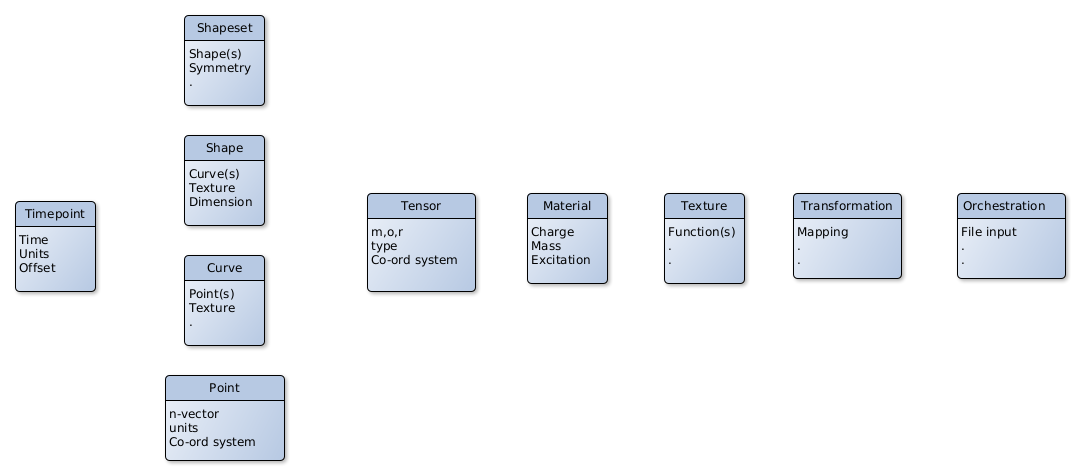
\includegraphics[width=0.7\textwidth]{./pics/baseclasses.png}}
\caption{\nep \ base classes.
\label{fig:baseclasses}}
\end{figure}

\begin{itemize}
\item
  Timepoint : point in physical time Attributes of time, units, offset
  (Alternatively just real scalar)
\item
  Point : point in \emph{n-D} space\\
  many make curve, shape;\\
  is particle location in \emph{n-D} ; Attributes of n-vector, units,
  coordinate system (Alternatively just real n-vector)
\item
  Curve : parts are one or more points, straight lines or textures
  or from CAD input or CSG input;\\
  many make shape;\\
  is shape boundary, is particle trajectory, is ray
\item
  Shape : parts are curves and textures, planar rectangles, or
  surfaces from CAD input or CSG input;\\
  many make Shapeset;\\
  is surface which aggregates as BC
\item
  Shapeset : parts are shapes, regular lattice, or volumes from CAD
  input or CSG input;\\
  is finite element geometry, is unstructured mesh, is surface geometry
  of body, is volume in \emph{n-D}, $n\geq 3$ ;\\
  helps defines field\\
  Attributes of degree of toroidal symmetry
\item
  Tensor : parts are $m$ numbers at a point, order $o$, type eg.\ 
  \emph{udd}, and density $r$ in \emph{n-D} coordinate system of type
  \emph{c};\\
  is ($m=3$, $o=1$, $n=3$) velocity, is ($m=1$, $o=3$,
  $n=3$) density,\\
  is ($m=1$, $o=0$, $n=3$) temperature, is ($m=3$, $o=0$,
  $n=0$) is array;\\
  many help make field (\emph{u} denotes contravariant, \emph{d} denotes
  covariant, \emph{c} defines cartesian, cylindrical, toroidal
  coordinates, $r=0$ usually)
\item
  Material : from database input ;\\
  helps make body, particle, many make matexture, plasma\\
  Attributes of charge, excitation level and mass
\item
  Texture : parts are mathematical library functions,
  particularly  mathematical library interpolation functions - see \Sec{mathematical-library-operations}\\
  aggregates as matexture, BC
\item
  Transformation : mathematical formula defining geometry
  transformations on point and tensor (co- and contra-variant) $\bf{\bar{x}}\rightarrow \bf{x}$
\item
  Orchestration : parts are from configuration file input see
  \textbf{Orchestration}, model, framework
\end{itemize}

\subsection{Aggregates}\label{sec:aggregates}

\begin{figure}
\centerline{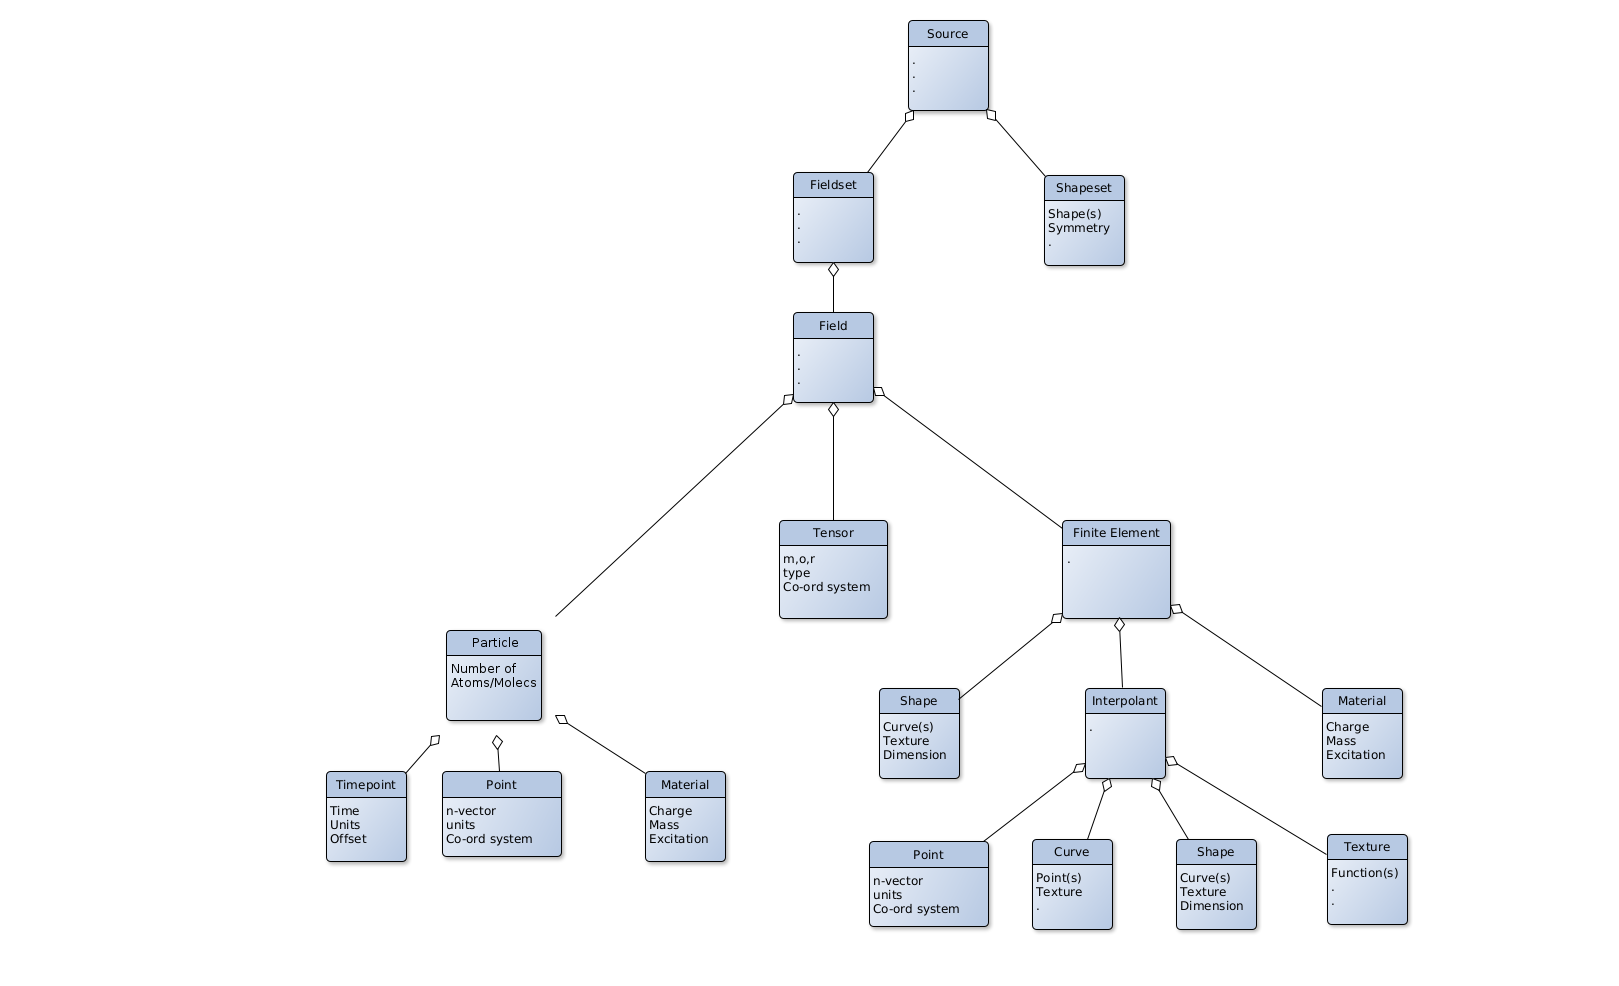
\includegraphics[width=0.7\textwidth]{./pics/aggregates.png}}
\caption{Aggregation of base classes to form a class `Source'.
\label{fig:aggregates}}
\end{figure}
\begin{itemize}
\item
  Particle : parts are location, velocity, material;\\
  Attributes of particle weight
\item
  Interpolant : parts are points, curves, shapes, textures, or
  timepoints, textures
\item
  Diagnostic : parts are DSL input instructions \textbf{Diagnostic
  Processing}, fieldset
\item
  FE (Finite element) : parts are shape, interpolant, material
\item
  Field : parts are tensors and finite elements, or particles;\\
  many make fieldset
\item
  Fieldset : parts are fields
\item
  DE (Differential equation) : parts are operators (DSL input), IC, BC
  and source
\item
  Model : parts are \textbf{Solution of DEs}
\item
  Source : parts are shapeset, fieldset. See \Fig{aggregates}.
\item
  Matexture : parts are materials, textures
\item
  Body : parts are shapeset, matexture
\item
  BC (Boundary Condition) : parts are surface, material, texture
\item
  GEOQ (Geometry plus B-Equil) : parts are shapeset, field
\end{itemize}

\subsection{Simple inherits}\label{sec:simple_inherits}

\begin{itemize}
\item
  HDS (Hierarchical Data Structure) : multi-octree, is a shapeset
\item
  Trajectory : particle position as time varies, is a curve
\item
  IC (Initial Condition) : is a fieldset
\end{itemize}

\subsection{Solution of Differential Equations}\label{sec:solution_of_des}

Use in part ABSTRACT CALCULUS and PUPPETEER patterns (cf.~GoF FACADE)
from Rouson et al. \cite{rousonxiaxu}, see \Sec{desi_patt}.

\subsection{Diagnostic Processing}\label{sec:diagnostic_processing}

\begin{enumerate}
\def\labelenumi{\arabic{enumi}.}
\item
  Read configuration file
\item
  Determine whether any diagnostic needed at present physical time
\item
  Select input fieldset
\item
  Select diagnostic type, use in part ABSTRACT CALCULUS from Rouson et
  al. \cite{rousonxiaxu}

  \begin{itemize}
  \item
    Initial logs

    \begin{itemize}
    \item
      UUID
    \item
      Key input data
    \item
      Key properties, eg. LCFS
    \end{itemize}
  \item
    Combinations of

    \begin{itemize}
    \item
      Field / quadratic field (eg. power, flux quantity) / general
      formula
    \item
      Point, line integral, surface integral, volume integral
    \end{itemize}
  \item
    Mass/charge, momentum/current and power balances
  \item
    Turbulence statistics - cross-correlations, spectra (not particle,
    ray)
  \item
    Difference between solutions/experiment (RMS as `skill') (not
    particle, ray)
  \item
    See ``emergent physics as diagnostic'' in imas\_objects.tex
  \end{itemize}
\item
  Calculate output fieldset
\item
  Set output format
\item
  Output fieldset to disk, screen
\end{enumerate}

\subsection{Orchestration}\label{sec:orchestration}

\begin{enumerate}
\def\labelenumi{\arabic{enumi}.}
\item
  UQ Framework VECMAtk and Fab\nep
\item
  GUI
\item
  CLI
\item
  Possible restart (OLYMPUS logic, Fig.1 of \cite{y2re312})
\item
  \textbf{Initialise} from functions.md
\item
  \textbf{Solution} from functions.md
\end{enumerate}

\clearpage
\newsection{Execution sequence}{sec:DDF_sequence}
\subsection{Preprocessing and
components}\label{preprocessing-and-components}

\begin{itemize}
\item
  Convert equilibrium B-field to standard format (ie. a standard
  resembling EQDSK)
\item
  Convert n-D geometry (NURBS) to opensource format
\end{itemize}

\subsection{Initialise}\label{sec:initialise}

\begin{itemize}
\item
  Convert n-D mesh to readable format
\item
  Assign boundary conditions to mesh (finite element by finite element)
\item
  Validate inputs (eg. Python Cerberus)
\item
  Initialise fields, possibly exploiting toroidal symmetry

  \begin{itemize}
  \item
    using sources, calculate with possibly simplified dynamics
  \item
    semi-analytically (Gaussian in vel. space)
  \item
    random perturbations
  \item
    from disk file
  \item
    from previous calculation
  \item
    apply operators to field (eg.\ EQDSK data \(\rightarrow\) B-Equil)
  \item
    combine vacuum field and B-Equil
  \end{itemize}
\item
  Calculate LCFS
\item
  Normalise field
\item
  Distribute mesh across processors
\item
  Distribute particles across processors
\end{itemize}

\subsection{Solution}\label{sec:solution}

\begin{itemize}
\item
  Extra outer loop over parameters (UQ Framework)
\item
  Outer loop over time
\item
  Inner loop over solver

  \begin{itemize}
  \item
    loop over particles
  \item
    loop over rays
  \end{itemize}
\item
  More deeply nested iteration
\item
  Convergence test
\item
  Rouletting particles
\item
  Particle collision

  \begin{itemize}
  \item
    with geometry
  \item
    with other particle
  \end{itemize}
\item
  Adaptive meshing
\item
  Construct surrogates (UQ Framework)

  \begin{itemize}
  \item
    Reduce in n-D (\(n \rightarrow n-1\))
  \item
    Combine particles
  \item
    Replace particles by FE
  \item
    Smoothing
  \item
    Gyro-averaging
  \item
    Sparse models for Data Assimilation (via SINDy)
  \item
    Gaussian Process
  \item
    Polynomial Chaos Expansion
  \item
    Active Subspaces
  \item
    PGD
  \end{itemize}
\item
  Connect surrogates (UQ Framework)
\end{itemize}

\subsection{Assortment}\label{sec:assortment}

\begin{itemize}
\item
  Calculate HDS from Field geometry data
\item
  Intersect triangle with cuboid
\item
  Calculate surface normal and tangents, curvatures
\item
  Calculate curve tangent and normals, torsion, curvature
\item
  Calculate volumes
\item
  Locate point in field element geometry data
\item
  Select algorithms
\item
  Label with physical units, array dimensions, transformations
\item
  Increase in n-D (\(n \rightarrow n+1\))
\item
  Replace FE by particles
\item
  Evaluate FE representation at set of points
\end{itemize}

\subsection{Diagnostics}\label{sec:diagnostics}

\begin{itemize}
\item
  Calculate terms in power balance
\end{itemize}

\subsection{Utilities}\label{sec:utilities}

\begin{itemize}
\item
  Format conversion
\item
  sorting
\end{itemize}

\subsection{Mathematical library operations}\label{sec:mathematical-library-operations}

\begin{itemize}
\item
  FFT (FFTW package)
\item
  linear algebra
\item
  quadrature
\item
  optimisation
\item
  geometry transformations on point and tensor
\item
  Interpolation STRATEGY to select among

  \begin{itemize}
  \item
    splines (2-D, 3-D)

    \begin{itemize}
    \item
      regular (de Boor)
    \item
      local
    \item
      Weiland
    \end{itemize}
  \item
    Fourier interpolation
  \item
    rational interpolation
  \item
    Lagrange interpolation (after Trefethen)
  \end{itemize}
\end{itemize}

\newsection{Design patterns}{sec:desi_patt}
The design patterns likely to be most relevant to \nep \ are described
in refs~\cite{y2re332,y2re333}.

The PUPPETEER pattern appears to be
exclusive to the works of Rouson~et~al, hence is described further here.
It is directed towards the calculation of the Jacobian of multi-component
systems typically needed for Newton-Raphson type solution of update equations.
The idea is that the puppeteer need only know which blocks of the Jacobian
matrix are nonzero, although the puppets need to be capable of forming derivatives
with respect to all state variables.
\begin{figure}
\centerline{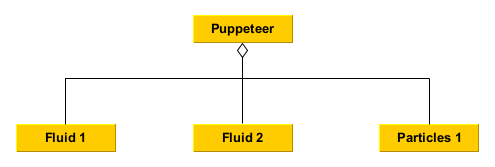
\includegraphics[width=0.95\textwidth]{./pics/puppeteer_wab.png}}
\caption{
PUPPETEER pattern. Each puppet (`Fluid~1', `Fluid~2', `Particles~1') may include terms  involving 
the other puppets. For example, suppose the puppet for `Fluid~1' has terms involving also `Particles~1'
variables (but not `Fluid~2'), then the puppeteer can request derivatives of the puppet's terms both
with respect to `Fluid~1' and `Particles~1' variables, but knows not to ask for derivatives with respect
to `Fluid~2' variables.
\label{fig:puppeteer_wab}}
\end{figure}


% Sommerville  - System architecture
% Sommerville  - System requirements specification
% Sommerville  - System models
% Sommerville  - Appendices
% Smith  - Requirements  - Specific System Description  - Problem Description  - Physical System Description
% Smith  - Requirements  - Specific System Description  - Solution Characteristics Specification
% Hewitt  - Application Design  - Design patterns
% Smith  - Design Specification
% Hewitt  - Application Design  - Scalability and performance
% Hewitt  - Application Design  - Extensibility
% Smith  - Requirements  - Likely Changes
% all of Hewitt  - Data Design
% Smith  - Requirements  - Requirements  - Nonfunctional Requirements
% sections 1 and 2 of Hewitt  - Infrastructure Design

\newchapter{Management File}{sec:MGT}
The Management File (MGT) is a developer generated file
that describes the management features of the software project notably,
organizational breakdown and responsibilities, work activities breakdown,
selected life cycle, deliveries, milestones and new risks.
% Smith  - Development Plan
% Hewitt  - Infrastructure Design  - Software distribution
% Hewitt  - Business Design  - Governance
Note that the report~\cite{y2d34} entitled ``Development Plan" is primarily
concerned with the documents needed for managing the project, and how
they should be arranged as a website.

The range of levels of detail and implicitly computational cost (from Exascale 
down to laptop) will follow from the projected development via a sequence of 
\papp s of increasing complexity and detail. This process is expected to 
enable an enhanced selection through experience and feedback, of
\begin{itemize}
\item a common set of software objects/classes
\item computer languages suitable for design with 'separation of concerns
\item numerical algorithms
\item user interfaces
\item interfaces to databases and coupling to codes not conforming to \nep \ standards
\end{itemize}
Selections will be recognised as better if they lead to improvements in 
scalability and portability, reliability and resilience, extensibility, and 
ease-of-use. 


\newsection{Introduction}{sec:MGT_intro}
Webpages on this site concerning management details are taken from the
report~\cite{y3re314}, based largely on the work of Ben Dudson, which
presents guidance concerning the mechanics of an opensource development
by a community distributed  across different sites and organisations,
intended to produce software intended for widespread long-term usage.
Parts of ref~\cite{y3re314} relate more to 
the technical specification~(TS) and are reproduced in \Sec{TS_sw_response},
another part concerns operational aspects~(OP), see \Sec{OP_MGT}.
Its recommendations are broadly consistent with those laid out by Bungarth \&
Heister~\cite{Ba13What}, and in particular those for the usage of \T{git}
conform to practice recommended by the ITER organisation.
This document is not the place for a general discussion of software engineering practices,
and does not cover code coupling, both of which topics are discussed in the open literature,
see in particular Lawrence~et~al~\cite{La18Cros} for HPC software engineering and
Belete~et~al~\cite{Be17over} for code coupling,
also see other \nep \ reports, particularly refs~\cite{y2re312,y2re333,y3re72}.

Ref~\cite{y3re314} assumes that all the community has signed up to a ``Charter"
which for \nep \ appeared as report~\cite{charter}, reproduced in \Sec{charter}.
The guidance\cite{y3re314}  includes  important issues that need to be agreed as early as possible.
%drawing on the ``Development Plan" document~\cite{y2d34} and on
These include practical points concerning frequency of meetings, code review etc.,
designed to ensure efficient collaboration between a wide group of project partners. 
%It is important to distinguish use-cases. There appear to be three
%use-cases worth treating separately:
%\begin{enumerate}
%\item code produced for immediate and local use only, eg\. to test out an idea or to illustrate a
%scientific paper.
%\item software for long-term use, where execution speed is time-critical, eg\. for real-time
%control or inter-shot discharge analysis.
%\end{enumerate}
%This note relates most closely to the third case.
The guidance document\cite{y3re314} also seeks not merely to prescribe, but to
give compelling arguments for the choices made in respect of guidelines.
Acknowledging the possibility of diagreements, it states that efforts will be made to ensure
consensus or at least agreement between the two most affected project partners
on any decisions taken. However, in the event of continuing disagreement, the technical
leader or `Lead' for the project will ultimately decide on the basis of technical
evidence presented, subject to ratification by higher management.

One general rule is always to allow two options (`rule of two'), intended to enable exploitation 
and possible incorporation of any promising new software (eg.\ package, library or language)
or relevant algorithm which emerges during the course of the project.
Since however, each option doubles the potential cost of developing and maintaining software,
a good case must be made to the Lead for a new option, and the innovator include provision
for retiring one of the existing options should there already be two. Implicitly
thereby, as discussed at the end of \Sec{lang}, a third exploratory option is also allowed.

A similar recommendation (rather than rule) regarding both code and documentation is to
`write once, re-use many times'.
This to a large extent explains a preference for the \LaTeX \ {\tt lwarp} package as enabling
multiple reuse of the same text and mathematical expressions in different
documents and on different webpages.


%The guidelines for a development are set out in the body of this document in an
%arrangement consistent with the concordance, such that separate sections
%correspond to the different documents/web-pages required.


\clearpage
\newsection{Management}{sec:MGT_MGT}

Meetings, whether on-line or in-person are regarded as critical for good collaboration,
and are discussed in \Sec{meet}. The other key collaborative element centres
naturally on the software, where use of the \T{git} control system, see \Sec{version}
and consequent use of repositories, see \Sec{repo}, is becoming universal.

\subsection{Meetings and Workshops} \label{sec:meet}

To start the project and any notable identifiable piece of work
within it, a kick-off meeting should bring
together all partners who will contribute significant code to the
project.  The aim of this meeting will be to build personal links
among the team, and to establish community practices consistent with the charter.
Efforts should be made to build consensus and
a community spirit within the project team.

A regular project planning and monitoring meeting should be set up,
at least monthly. Its agenda should include short updates on progress of
each project component, and focus on the project planning and
coordination. In addition, a separate series of seminars and training
should be organised, where each partner might give a longer talk on an
aspect of their work, for example showing other partners how to use
recently developed capabilities.


Development and collaboration mechanisms should include:
\begin{enumerate}
\item A system of code repositories for version control (eg.\ \T{github})
\item Automated testing infrastructure (eg.\ \T{github} actions)
\item Documentation infrastructure, ie.\ as a website
\item A repository for long-term storage of large files, records of
meetings, presentations etc. (eg.\ Google shared drive)
\item A chat/messaging service such as Slack, to facilitate interactions
between developers
\end{enumerate}
As these are established, a series of training workshops should be
arranged. These should include talks on the ``high level" objectives, 
on the near-term plans of each partner, and also hands-on training in
the tools being used. 


\subsection{Version control} \label{sec:version}

The standard \T{git} version control system should be used; there is no
viable competitor to this in terms of capabilities, widespread adoption,
or integration into other tools and services (eg.\ \T{github}).

A common complaint against \T{git} is the user interface, which can be intimidating 
to new users. There are very strong reasons why even programmers with
plenty of other experience, should seek guidance and preferably training
in use of the command line interface~(CLI). For those who have time enough to attempt to do so without, 
a few hints are provided: 
\begin{enumerate}
\item The complexity of the interface can be mitigated by restricting usage
to a few well-chosen subcommands such as \T{clone}, \T{add}, \T{commit}, \T{push}, \T{pull}, \T{diff}, \T{log} and \T{status}.
\item  Exercise caution before using other
subcommands or new options to the core subcommands, eg.\  by first committing all files, adding a suboption
which indicates what will be done without actually modifying any files, and avoiding 
forcing options.
\item For the purpose of the key subcommands such as `pull' and `push', it is important
to remember than these are are defined from the user's point-of-view,
so that `pull' brings source from the repo towards the user, and `push' sends it away.
There are other non-intuitive aspects so that it is important to study very carefully the
description of any new sub-command/option and particularly its ordering of options.
\item Since the software is widely used, error messages can invariably be `googled'
for further explanation.
\item Should conflicts occur, these are recorded by the insertion of strings `+++\ldots',
`\verb->>>>...-' and `\verb-<<<<...-' in disc files to indicate lines where the clashes lie. Many users
find resolving conflicts very difficult on the basis of such information,
however making up for  the absence of a GUI mechanism within \T{git} to do this,
it is possible to integrate GUIs such as \B{meld}, being aware of possible system dependences.
\end{enumerate}

Otherwise, the experience of \T{git} can be mitigated through:
\begin{itemize}
\item Training: Links to training material for adopted tools should be made available
as part of the project documentation. This should be supplemented by training,
both one-to-one and as part of a programme of talks and training.

\item Adoption of, and training in, tools to provide easier interfaces. \T{github} itself
allows browsing of history; \T{Magit} is an excellent interface integrated into Emacs;
and similar tools exist for eg.\ Visual Studio Code.
The ITER organisation uses \T{bitbucket} and UKAEA uses \T{gitlab}.
\end{itemize}
%Training in use of \T{git} should make clear that pretty every much aspect of the
%CLI is unsatisfactory and similar features should be deprecated in the new development. 


\subsection{Code repositories} \label{sec:repo}

The structure of \exc \  will result in a number of different
components, experimental \papp s, and increasingly complex
applications. There are two main different approaches as to how these different
components could be split between git repositories, namely (1) Several large code
bases are kept in a single repository (a `monorepo') and (2) 
projects are kept in  separate repositories, with
dependencies being included as \T{git} submodules. 

%Advantages of `monorepos' include simplified dependencies, synchronisation of
%changes to different components, and a central location for documentation.
%The main argument for having separate repositories is for the occasion when several components
%already pre-exist as separate repositories. For new modules, strong
%coupling between components should be discouraged, so that components
%can be reused in a range of applications. %The separate repositories
%enables finer control over access rights, though this can imply
%additional barriers to shared code ownership.

Adopted is a compromise approach whereby:
\begin{itemize}
\item A \T{github} `organisation' \url{https://github.com/ExCALIBUR-NEPTUNE}
was created to host new repositories. 
%(The names ``Neptune" and ``Excalibur" were taken, but
%``excalibur-neptune" was available, for example.)
Organisations allow permissions for groups of administrators and
developers to be managed, and this is currently restricted to community members, so
that it is important to be `logged in' to access their components.
\item Individual components and \papp s are hosted in separate repositories under this
organisation. These contain the code, unit tests, documentation etc.
specific to these components.
\item Reports produced as part of the \nep \ project, unless they
contain commercially sensitive information, are to be found in the
repository~\cite{xpndocswebsite}.
\item A central repository under this 
organisation includes components as sub-modules. These could be
organised into a directory structure, with documentation explaining the relations
or coupling between components. In this repository should go:
\begin{itemize}
\item Integration tests which couple components and ensure that they work together
\item Documentation of the interfaces between components, project conventions
(eg.\ style guides), and overall project aims.
\end{itemize}
Sub-modules are pinned to a particular \T{git} commit, so that at any
point the versions included are those which are known to work with
each other. A developer who wants the latest version of a component
should clone the individual repository, while a user who wants
something that ``just works" should clone the central repository.
\end{itemize}
(There is the disadvantage of a tie specifically to \T{github}, but loss
of the `organisation' capability would be expected to be an inconvenience rather
than a disaster for a project.)

\subsection{Development workflow} \label{sec:develop}

The standard \T{git} work flow has been adopted, since this is widely
familiar and has been developed as best practice based on industrial
experience. Exceptions are allowed for minor issues, such as typographical
errors and broken links in documentation.

Each code component maintains a \T{main} branch (often referred to as the `master'
as in `master copy'), which can only be modified
through a pull request mechanism which ensures peer review and testing. Bug fixes
and feature development are done in separate branches, either in the same
repository, or in forked repositories. When someone encounters a bug, or wishes to
develop a new feature, the recommended approach ise:

\begin{enumerate}
\item An issue is opened, describing the bug or feature request or proposal. This
allows discussion of the issue, and possible approaches to addressing it.
\item A pull request is opened as early as possible, marked ``Work in
progress" or similar. This can contain only minimal code or outline
of the code structure. This links to the issue, lets other people
know that it is being worked on, and enables peer review and input
into the development direction.
\item Once ready for merging, and consensus has been reached that the proposed change
should be made, then it is merged.
\end{enumerate}

If a code is sufficiently large, then a further degree of separation between
the stable \T{main} branch and active development is needed. A common pattern
is to only branch off and merge features into a  \T{next} branch. Periodically
this branch is merged into \T{main} as a new release, once the new features 
are judged to be sufficiently mature and tested.

Whether into \T{main} or \T{next}, pull requests should be reviewed
using a checklist the remind the reviewers. 
Review involves testing, aspects of which are addressed in \Sec{test}.

It must be stressed that code review is not a job separate from
code development: {\bf All developers should be expected to participate in
and carry out code reviews}. Reviewing code benefits not only the
original author, but also the reviewer. Through the discussion, it
contributes to a sense of shared ownership of the code base, and
spreads good practices. There is the implication that code should be
written `for the other guy', ie.\ so that the other guy can understand it
without much difficulty.  It also ensures that at least two developers
know how each part of the code works.

\subsection{Code release}

Code releases should be a regular occurrence.
Code release helps with project branding and user engagement,
and ensures that the project is seen as active.
It also helps project administration by ensuring new features are shared in a timely fashion,
and by reducing the number of long-lived divergent branches. 

The project \nep\ codebase contains \papp s, and infrastructure code that interfaces them.
A code release will consist of a version of this infrastructure code, 
plus commit hashes that fix the versions of the \papp s.
As \papp s might be independent projects with their own established release cycle,
the following release policy applies only to the infrastructure code.
It is the recommended policy for new \papp s written under Project \nep.

Release numbering should follow (a modified) Semantic Versioning approach~\cite{semverwebsite}, summarized as
\begin{quote}
``Given a version number MAJOR.MINOR.PATCH, increment the:
\begin{enumerate}
  \item MAJOR version when you make incompatible API changes,
  \item MINOR version when you add functionality in a backwards compatible manner, and
  \item PATCH version when you make backwards compatible bug fixes.''
\end{enumerate}
\end{quote}
Here it is understood that ``API'' refers to user-facing interfaces;
APIs to functions internal to \papp s may break backwards compatibility in
MINOR releases.
There is however an absolute guarantee that no backwards incompatible changes
are made for end users in MINOR and PATCH releases, except those that arise
from fixing a bug.
That is, physics results are permitted to change in such releases if the new
release's results are ``correct'' and the previous release's results were
``wrong''.

It is also understood that releases with MAJOR number 0 are considered beta releases,
for which there are no guarantees of backwards compatibility.
 
Each release will be uploaded as a Zenodo\cite{zenodowebsite}
record with its own DOI.
This gives a clear citation for the project (to be included in the project's
README or CITATION.cff file),
while ensuring that developers receive credit for their work, without the need
for associating each release with a publication.
Encouraging researchers to use release versions and to cite by version number
also aids scientific reproducibility.

While some technical aspects of the release process can be automated,
many of the tasks, such as curating issues and writing release notes, are
inherently manual.
To prevent \nep\ relying on a single person to make releases,
the exact workflow will be codified and included in the project documentation.
An example of such a workflow for the GS2 project may be found
online~\cite{gs2website}.



\clearpage
%\section*{Acknowledgement}\label{sec:ackn2}
%%\emph{The support of the UK Meteorological Office and Strategic Priorities Fund is acknowledged.}

%Based on a document provided by Ben Dudson, ``Suggestions for ExCALIBUR community guidelines planning",
%dated December 16th, 2020.
\newsection{\exc \ Project \nep \ Charter}{sec:charter}
All members of the \exc \   \nep \   team should be aware that 
to meet the challenges of the \nep \   project, and the \exc \   overarching 
pillars, a distributed team of scientists, software engineers and architecture 
specialists from different UK institutions will be required to form a community 
around the \nep \  project (and will connect across the overarching \exc \   
programme). A high-level objective is to ensure that developed software is of 
the highest quality, implying a rigid requirement around the production of 
high-quality documentation and reproducible verification and validation tests 
for the codebase as it evolves. Since development work may transfer between 
institutions, it is important that common standards for documentation and 
testing be available and easy to deploy. The initial \nep \   exploratory 
\Papp s~may be written in a range of languages including for example Python, 
C++/DPC++, Object Fortran or Julia, however it is envisaged that there will be 
an emerging steer towards a reduced set of languages and technologies to ensure 
interoperability across the \nep \   software stack, ultimately leading to 
coupled simulations covering all the physics necessary to deliver an 
``actionable'' simulation for the plasma edge. It is not yet clear for 
example whether SYCL, Kokkos or OpenMP~5 will offer the most performance 
portable and sustainable solution for \nep.
The team is therefore expected to be agile and amenable 
to change once it is clear which are the most promising long--term solutions. 
For example, a selection of SYCL for the long-term framework/code(s) would 
force refactoring of any code that is not consistent with a \nep \   library and 
code base instantiated in DPC++, and where feasible, team members 
should support this process.


Source code for all development should be accessible by the 
entire \nep \   team and all tests should be repeatable by different workers 
without the need for re-training and/or any possible confusion as to the 
procedures and metrics needed to declare a 
test successful.

\nep \   will be developed as a sequence of `core' \Papp s 
(to be distinguished from other \Papp s designed to test some novel 
technique). Core \Papp s will all need a documentation and testing framework, 
which must be agreed between all partners for the entire project. This will 
require developers to work closely with UKAEA and other team members.

A commitment is also expected by all parties to help UKAEA 
and the Met Office (as SRO for \exc) to publicise the project and build a 
fully connected community across the \exc \   programme, UKRI and Academia, 
focused upon a team of approximately twenty UK Fusion use case experts. This will 
be essential for meeting the grand challenge goal of developing a 
state-of-the-art, Exascale targeted, UK-based plasma physics simulation 
capability for the tokamak edge plasma (see Science Plan~\cite{sciplan}). 



All Core \Papp s and related infrastructure/documentation 
across the \nep \   project should meet the demands of the Code Structure and 
Coordination work package FM-WP4 in so far as the developing project standards:
\begin{itemize}
\item[$\bullet$] adopt a consistent choice of definitions (ontology) of 
objects or equivalently classes,
\item[$\bullet$] adhere to clearly defined common file formats and 
interfaces to components for data input and output.
\item[$\bullet$] provide suitably flexible data structures for common 
use by all developers,
\item[$\bullet$] are established through good scientific software 
engineering best practice,
\item[$\bullet$] demonstrate performance portability and exploit agreed 
DSL-like interfaces where possible targeting Exascale-relevant architectures,
\item[$\bullet$] can be integrated into a VVUQ framework and
\item[$\bullet$] are embedded within a coordination and benchmarking 
framework for correctness testing and performance evaluation.
\end{itemize}

In order to meet Strategic Priorities Fund terms around eligibility, 
and to steer the project towards a modular platform where developments 
across all partners can be integrated into an eventual code or platform 
available for open use by the European fusion community, a requirement 
is that all \exc \ \nep \ Grant beneficiaries make technology / source 
code developed through the programme (foreground Intellectual Property) available as open 
source under a programme--wide permissive license (currently selected as 
3-clause BSD for core/foundational infrastructure~\cite{bsd3clause}). Government 
Digital Service guidance (to which the project subscribes), discussing 
the benefits of open versus closed technology/software/data can be found 
in~\cite{os,os2}.


% Smith  - Development Plan
% Hewitt  - Infrastructure Design  - Software distribution
% Hewitt  - Business Design  - Governance

\newchapter{Maintenance File}{sec:MF}
The Maintenance File (MF) is a developer generated file
that describes the planning and status of the maintenance, migration and retirement activities.
% Sommerville  - System evolution
% Hewitt  - Application Design  - Availability
% Hewitt  - Infrastructure Design  - Maintenance
% Hewitt  - Application Design  - Maintainability

% Sommerville  - System evolution
% Hewitt  - Application Design  - Availability
% Hewitt  - Infrastructure Design  - Maintenance
% Hewitt  - Application Design  - Maintainability

\newchapter{Operational Documentation}{sec:OP}
The Operational Documentation (OP) consists of the Developer Manual~\Sec{DevMan} and
the User Manual~\Sec{UMan}. It is important that
the user's experience of the software feeds back into the instructions
as to how to use the software, and mechanisms for achieving this end appear
in \Sec{feedback}.
%Everyone hates writing documentation, it gets written badly, and therefore no-one uses it. 
%Therefore no-one funds doing it, and documentation is bad. %Smith
%As with other overheads in software development, expects that work required will reduce over
%time as it becomes standard practice but need to convince people to adopt it in the first place!

\newsectionnobreak{Documentation Generally}{sec:OP_MGT}
%\section{Documentation Generally}\label{sec:OP_MGT}

\subsection{Documentation} \label{sec:doc}

Documentation refers to a particular version of the code. It should therefore be
dynamic, under version control, and tightly coupled to the source code itself. 

\begin{itemize}
\item All new code features should be documented, and this should be checked as
part of the peer review process.
\item Within the code, comments should use a convention, such as that
accepted by \F{Doxygen},
to document the intent of functions, and any assumptions on their
environment, input or outputs.
\item Alongside the code \T{README} files explaining the file/directory layout 
typically use the Markdown format due to its simplicity,
standardising on the variant defined by \F{Pandoc} as described in \cite{y2d34}.
\item The more formal documentation should be in a format which can
include elements such as equations, code blocks, graphs and figures.
It should also be easily convertible to other formats, and in
particular online documentation. \LaTeX \ as used to produce the current document
can be easily converted to .html as explained in ref~\cite{y2d34} provided
the restrictions (as to accepted packages) noted in the reference are observed.
\end{itemize}


\newsection{Developer Manual}{sec:DevMan}
\subsection{Testing} \label{sec:test}

Requirements before merging changes in \T{git} include:
\begin{itemize}
\item Tests must pass. (Merge blocking can be enforced eg.\ on \T{github}.)
\item The code must be in the standard style, which will be at least
partly enforced as part of the automated testing.
\item Documentation must be updated or added to reflect changes in the code.
\end{itemize}

\subsubsection{Source code testing} \label{sec:source}

Testing of code is essential to ensure correctness, reduce incidents
of accidental breakage or regression of code features, and enable code
changes to be made with confidence. These tests must be automated, and
as far as possible be ``unit" tests, which test isolated components of
the code. A strictly Test Driven Development (TDD) approach is not
always appropriate, but encouraging incremental development and
testing in small pieces has several advantages in terms of the
resulting code structure and maintainability:

\begin{enumerate}
\item It encourages the writing of code which has ``clean" interfaces ie.\ 
a well defined set of inputs and outputs, with minimal side channels (eg.\ 
global state).
\item Having to test components individually discourages strong coupling
between code, because then these dependency components have to be
``mocked" up in testing.
\item Good code test coverage makes later maintenance, modification and refactoring
of the code easier. The tests also function as a type of documentation
of the intended use of the code, and also of the corner-cases which may not
be obvious to a new user or developer.
\end{enumerate}

The most important types of tests are for correctness. These can use standard
services such as \T{github actions}, \T{Travis} etc. Performance is however
a crucial property of the code, and should also be monitored.

\subsubsection{Performance testing} \label{sec:perf}

It is useful to include timing information in test output, which is
then contained in the test logs. This is valuable as a quick way for
developers to observe the impact of changes on performance. It is
however not very accurate, especially under virtual machines on shared
hardware as is typical for testing services. These tests also only
typically use a small number of processors (less than four), usually without
accelerator support, making them of limited use in evaluating
performance of high performance code for the Exascale. 

Periodic testing of code versions on a range of hardware will be
needed to monitor performance, and catch performance regressions. This
could be carried out by a researcher, but the possibility of
automating this process and making use of services such as Amazon AWS
HPC and GPU servers. Studies carried to date indicate a lack of appropriate
software for ensuring performance portability and a consequent
need at least to enhance existing packages.



%
How to configure git

Option to add personal profile

Email address for support neptune@ukaea.uk

List of projects/packages

Quick links

Separate the subject from body with a blank line and limit the subject line to 50 characterss

Importance of Slack or Zulip

producing FMS reports collaboratively using git and mostly LaTeX some markdown,
markdown is not a standard, except very minimally, so I would demand compatibility with pandoc.

Zenodo indexing for s/w

How to Contribute

Community Code of Conduct see charter.tex
to include  Acknowledging and Citing

``Write code for people, not computers".
Literate programming. Interleaving documentation and codebase - minimises risk of code and documentation getting out of sync.
Use of Doxygen

C++ Core Guidelines (Bjarne Stroustrup, Herb Sutter)
\url{https://github.com/isocpp/CppCoreGuidelines/blob/master/CppCoreGuidelines.md}
Rules for high-performance or low-latency applications (otherwise Stroustrop's tour is 
reasonably comprehensive, includes chapters on numerics and
concurrency (parallelism)~\cite[\S\S\,14,15]{stroustroptour}
Mainly ``Don't optimize prematurely, but design to enable later optimization when it seems
it might be appropriate". Note that
Communication across nodes is \exc bottleneck at the Exascale.

Rouson~et~al's $12$~rules
\begin{enumerate}
\item Write code that comments itself.
\item Name all constants.
\item Make constants constant.
\item Minimize global data.
\item Make global data constant.
\item Provide global type parameters, including precision specifiers.
\item Provide global conditional debugging.
\item Declare intent for all procedure arguments.
\item Avoid side effects when possible, particularly in a function.
\item Make all derived type components private.
\item Indent loops and procedure/module executable statements.
\item Prevent implicit typing globally.
\end{enumerate}

Notes on DPC++ in ../ts/notes\_on\_dpc++.md

%\input{../t33/gamestruct.tex}
\subsection{Object Identification}\label{sec:objdisc}
Douglass~\cite[\S\,5]{douglass} has a description of object analysis which is well-suited
project \nep. His approach is to take the use cases, which for this purpose should
include the \papp s separately, and treat them carefully one after the other using
the strategies indicated in \Tab{objdisc}.
Each \papp\ should be carefully analysed and classes produced from the list of objects
before proceeding to the next.
\begin{table}[h]
\begin{center}
\caption{Key Strategies for Object Identification. After Table~5.1 from~\cite{douglass},
slightly amended.
All the strategies except the last, are concerned with identifying the objects listed.
\label{tab:objdisc}}
\begin{tabular}{|p{3.5cm}|p{12.0cm}|}
\hline
Strategy &  Description \\
\hline
\hline
Nouns  &  Used to gain a first-cut object list, the 
analyst underlines each noun or noun phrase in the problem statement and 
evaluates it as a potential object, class, or attribute. \\
\hline
Causal agents &  Identify the sources of actions, events, and messages; includes the 
coordinators of actions. \\
\hline
Services (passive contributors) &  Identify the 
targets of actions, events, and messages as well as entities that passively 
provide services when requested. \\
\hline
Messages and information flow &  Messages 
must have an object that sends them and an object that receives them as well 
as, possibly other objects that process the information contained in the messages.
There are many ways to identify the objects within a collaboration.  \\
\hline
Real-world items &  Real-world items are entities that 
exist in the real world, but are not necessarily electronic devices.  Examples 
include objects such as gases, forces,
blanket modules, etc. \\
\hline
Physical devices &  Physical devices include the sensors and actuators provided by the 
system as well as the electronic devices they monitor or control.  The resulting
objects are almost always the interfaces to the devices.
Note: this is a special kind of ``Identify real-world items". \\
\hline
Key concepts &  Key concepts may be modeled as objects.  Physical theories exist
only conceptually, but are critical scientific objects.  Frequency bins
for an on-line autocorrelator may also be objects. Contrast with
the ``identify real-world items" strategy. \\
\hline
Transactions &  Transactions are finite instances of interactions 
between objects that persist for some significant period of time. An example
is queued data. \\
\hline
Persistent information &  Information that must 
persist for significant periods of time may be objects or attributes.  This persistence
may extend beyond the power cycling of the device. \\
\hline
Visual elements &  User-interface elements that display data are objects within the 
user-interface domain such as windows, buttons, scroll bars, menus, histograms, 
waveforms, icons, bitmaps, and fonts. \\
\hline
Control elements &  Control elements are objects that provide the interface
for the user (or some external device) to control system behavior. \\
\hline
Apply scenarios &  Walk through scenarios using the identified objects. Missing objects
will become apparent when required actions 
cannot be achieved with existing objects and relations. \\
\hline
\hline
\end{tabular}
\end{center}
\end{table}

\newsection{User Manual}{sec:UMan}
ICD Interface Control Document (User Manual)

With video tutorial, quick start, installation, examples. %Smith
Examples use Jupyter - has Python and Julia interfaces. Binder shares a Jupyter notebook so
recipient can immediately execute in a browser
\newsectionnobreak{Feedback and Communication}{sec:feedback}
\begin{itemize}
\item Matrix chat - Slack?
\item Discourse group
\item Mailing list
\item Suggestion box
\item Weekly community meetings
\end{itemize}

%\input{../../t51/dimred.tex}

% \section{Developer Manual}\label{sec:DevMan}
% 
How to configure git

Option to add personal profile

Email address for support neptune@ukaea.uk

List of projects/packages

Quick links

Separate the subject from body with a blank line and limit the subject line to 50 characterss

Importance of Slack or Zulip

producing FMS reports collaboratively using git and mostly LaTeX some markdown,
markdown is not a standard, except very minimally, so I would demand compatibility with pandoc.

Zenodo indexing for s/w

How to Contribute

Community Code of Conduct see charter.tex
to include  Acknowledging and Citing

``Write code for people, not computers".
Literate programming. Interleaving documentation and codebase - minimises risk of code and documentation getting out of sync.
Use of Doxygen

C++ Core Guidelines (Bjarne Stroustrup, Herb Sutter)
\url{https://github.com/isocpp/CppCoreGuidelines/blob/master/CppCoreGuidelines.md}
Rules for high-performance or low-latency applications (otherwise Stroustrop's tour is 
reasonably comprehensive, includes chapters on numerics and
concurrency (parallelism)~\cite[\S\S\,14,15]{stroustroptour}
Mainly ``Don't optimize prematurely, but design to enable later optimization when it seems
it might be appropriate". Note that
Communication across nodes is \exc bottleneck at the Exascale.

Rouson~et~al's $12$~rules
\begin{enumerate}
\item Write code that comments itself.
\item Name all constants.
\item Make constants constant.
\item Minimize global data.
\item Make global data constant.
\item Provide global type parameters, including precision specifiers.
\item Provide global conditional debugging.
\item Declare intent for all procedure arguments.
\item Avoid side effects when possible, particularly in a function.
\item Make all derived type components private.
\item Indent loops and procedure/module executable statements.
\item Prevent implicit typing globally.
\end{enumerate}

Notes on DPC++ in ../ts/notes\_on\_dpc++.md

% \input{../t33/gamestruct.tex}
% \section{User Manual}\label{sec:UMan}
% ICD Interface Control Document (User Manual)

With video tutorial, quick start, installation, examples. %Smith
Examples use Jupyter - has Python and Julia interfaces. Binder shares a Jupyter notebook so
recipient can immediately execute in a browser
\newsectionnobreak{Feedback and Communication}{sec:feedback}
\begin{itemize}
\item Matrix chat - Slack?
\item Discourse group
\item Mailing list
\item Suggestion box
\item Weekly community meetings
\end{itemize}

% \input{../t51/dimred.tex}

\newchapter{Proxyapps}{sec:proxyapps}
A number of proxyapps have been written in order to provide initial \nep \ proofs-of-concept and to test relevant 
numerical physics.  This section provides brief outlines and links to relevant code repositories.
\newsection{Nektar-Driftwave}{sec:NektarDriftware}
Nektar-Driftwave solves the 2D Hasegawa-Wakatani equations describing drift-wave turbulence.  The equations are, for
vorticity $\zeta$, number density perturbation $n$, and electrostatic potential $\phi$,

\begin{eqnarray}
\frac{\partial \zeta}{\partial t}+[\phi, \zeta] &=& \alpha (\phi-n)\\
\frac{\partial n}{\partial t} +[\phi,n] &=& \alpha (\phi-n)-\kappa \frac{\partial \phi}{\partial y},
\end{eqnarray}

where $[a,b] \equiv \frac{\partial a}{\partial x} \frac{\partial b}{\partial y} - \frac{\partial a}{\partial y}
 \frac{\partial b}{\partial x}$.

In the above, $\alpha$ is the adiabaticity operator (taken to be constant) and $\kappa$ is the background density 
gradient scale length.  The electrostatic potential is related to the vorticity by Poisson's equation $\nabla^2 \phi 
= \zeta$.

The main system is implemented as an advection problem using a discontinuous Galerkin formulation which provides numerical
stabilization meaning that the usual hyperviscosity term is not required.  The Poisson solve is implemented in a 
continuous Galerkin formulation. 

The example provided tracks the nonlinear evolution of an initial Gaussian spatial density perturbation to a
 turbulent quasi-steady state.  See the internal report \cite{y3re222} for a presentation of the output and a 
comparison with published results.

Nektar-Driftwave is publicly available at \url{https://github.com/ExCALIBUR-NEPTUNE/nektar-driftwave}.  


\newsection{Nektar-Diffusion}{sec:NektarDiffusion}
Proxyapp capable of simulating 2D diffusion with arbitrary symmetric diffusivity tensor, based on Nektar++.  The
equation solved, for diffusivity tensor $D$, temperature T (in the case where the diffusing quantity is heat), and 
time $t$, is

\begin{equation}
\frac{\partial T}{\partial t} = \nabla \cdot \left ( D  \nabla T \right ). 
\end{equation}  

The problem is motivated by the fact that a characteristic of magnetically-confined fusion devices is that diffusive 
transport is strongly anisotropic, with heat transport in the direction of the magnetic field lines being favoured 
(ratios in the components of the diffusivity tensor of up to approximately $10^6$ are physically-motivated).

A typical scenario for the proxyapp is a domain containing linear, parallel magnetic fieldlines making 
angle $\theta$ with the horizontal axis, with a heat source implemented as a Dirichlet boundary condition on the 
left-hand-side vertical boundary, resulting in the diffusive transfer of heat to the lower domain boundary.  The 
interest is in small incident angles as these represent configurations in which the power incident on the wall of a 
nuclear fusion reactor (and hence the likelihood of damage) is minimized.

A number of examples are included, including time-dependent and steady-state problems in the type of geometry
 described above.  There is also an example of 2D semi-annulus in which the field-lines are circular arcs.  See the 
internal report \cite{y3re222} for an presentation of the relevant outputs.

Nektar-Diffusion is publicly available at \url{https://github.com/ExCALIBUR-NEPTUNE/nektar-diffusion}.


\newsection{Nektar-1D-SOL}{sec:Nektar1DSOl}

The Nektar-1D-SOL proxyapp models plasma transport in the scrape-off layer (SOL).
The SOL is treated as a 1D flux tube, with mass being added continously near the centre of the domain and flowing out to a divertor at either end.
Neutral species are ignored and the plasma is assumed to have an ideal-gas equation of state.

The proxyapp was built using Nektar's solver framework and is based on existing solver types that were designed for unsteady advection problems.
It adopts a similar approach to that used in the \textsc{soldrake} code described in section 4 of the internal report \cite{y3re222}.
The starting point is a set of non-dimensionalised equations describing the evolution of SOL density, momentum and energy, which were derived in \cite{detach-rp2}:

\begin{align}
    U_r \frac{\partial n}{\partial t} &= 
        - \frac{\partial }{\partial s}(nu)
        + S^n, \label{eqn:n}\\
    U_r \frac{\partial }{\partial t} (nu)&= 
        - \frac{\partial }{\partial s} (nu^2)
        - \frac{\partial }{\partial s} (nT)
        + S^u, \label{eqn:u} \\
    U_r \frac{\partial }{\partial t} \left( (g-2)nT + nu^2  \right) &= 
        - \frac{\partial }{\partial s}(gnuT + nu^3)
        + \kappa_d \frac{\partial^2  T}{\partial s^2}
        + S^E. \label{eqn:T}
\end{align}
The relative weight of time-dependent terms, $U_r$, is set to unity and the diffusivity coefficient, $\kappa_d$, to zero, yielding a system that closely resembles the compressible Euler equations.
Source terms and boundary conditions are then chosen so as to simulate mass deposition at the domain centre due to cross-field-line transport, and sonic outflow at each end (see \cite{y3re222} for a detailed description).
The domain is discretised using the Discontinous Galerkin method and time integration is performed using a 4$^{\rm th}$ order Runge-Kutta scheme.

Running the proxyapp produces a number of output files containing the values of the $n$, $nu$, and $E$ fields for each fluid element, which can be postprocessed using Nektar's `FieldConvert` tool to produce equilibrium profiles for $n$, $u$, and $T$.
These profiles closely match the analytical solutions derived in \cite{detach-rp2} and the results obtained using the \textsc{soldrake} code.

Nektar-1D-SOL is publicly available at \url{https://github.com/ExCALIBUR-NEPTUNE/nektar-1d-sol}.


\newsection{FabNEPTUNE}{sec:FabNEPTUNE}

Intended as a general tool for running NEPTUNE workloads, FabNEPTUNE is a plug-in for the FabSim3 Python-based toolkit
 for scientific workflow automation.  The framework generally enables the execution of simulation and analysis workloads
 on HPC via one-liner commands, automation of coupled models, facilities for reproducibility, and tools for ensemble
execution.  The framework offers also integration with the VVUQ toolkit SEAVEAtk. 

The current implementation of FabNEPTUNE is set-up to run simulations of heat transport by fluid convection, in 2D and
 3D, using the incompressible Navier-Stokes solver of the Nektar++ spectral/hp finite element framework.  The test 
problem simulates a fluid-filled rectangular cavity subject (via Dirichlet boundary conditions) to a specified 
horizontal temperature gradient, which leads to the generation of a convective circulation as fluid rises up the hot 
side and descends the cold.  There are two main control parameters represented by the dimensionless Nusselt and 
Prandtl numbers, with the former being a measure of the size of the applied temperature gradient - tuning this 
allows access to conductive, laminar-convective, and turbulent regimes.  This problem is relevant to fusion by 
analogy (\cite{Wi19Stab}) and is also a demonstration of the Nektar++ code.  See the internal reports \cite{y3re61,
y3re62} for numerical studies of the 2D convection problem using Nektar++.

FabNEPTUNE is publicly available at \url{https://github.com/UCL-CCS/FabNEPTUNE}.


\input{proxyapps/moment\_kinetics}

\newsection{NESO}{sec:NESO}

NESO is an implementation of a 1+1D solver for the Vlasov-Poisson problem in which the matter component is 
treated using particle-in-cell (PIC).  The electric field is taken to be purely electrostatic and is calculated by 
solving a 1D Poisson equation using a Fourier transform.This is a prototype for the particle problem to be treated by
 more advanced NEPTUNE proxyapps and also provides a demonstration for the use of multiple repositories and workflows
 for different code components.  

The code is implemented in SYCL (DPCPP and hipSYCL).

NESO is publicly available at {https://github.com/ExCALIBUR-NEPTUNE/NESO}. 



\newchapter{Reference Material}{sec:REF}
% Sommerville  - Glossary
% Smith  - Requirements  - Reference Material
% Smith  - Requirements  - Specific System Description  - Problem Description  - Terminology and Definitions
% Hewitt  - Infrastructure Design  - Standards and guidelines and conventions
% Hewitt  -  Acronyms and Symbols
\newsectionnobreak{Conventions for Report Writing}{sec:conv}
The project has strict standards in respect of conventions even in reports
that contain no code, ultimately to support the `write once, use many times' concept,
so that text may be cut, edited and pasted into source code, or indeed used safely to define
variable names, constraints on their values and physical dimensions.
Thus, since many compilers support only ASCII characters, only ASCII is allowed
in reports. Similarly, very long lines (typically arising from MS Windows wordprocessing)
should be split at the ends of sentences, and preferably so that maximum line length
is $120$~characters. A number of tools are available in \T{tex/importools}.
Contributors may use their style of choice for both reports (and code) provided
they follow systems that allow for automatic conversion to the conventions
expected in the \nep \ repositories, and are prepared to help construct gitlab runners and
github hooks to this end. However, it will be generally found easier to use \LaTeX \ and
bibtex as indicated below.

For shorter documents it is acceptable to use Markdown in the `dialect' defined by
\F{PANDOC}, see Annex~A of~\cite{y3re314}. Resulting .md files frequently convert
straightforwardly to \LaTeX \ format, using the md2tex.bash script from \T{tex/importools}.


\subsection{General textual issues}\label{sec:REF_text}
It is helpful to use \LaTeX \ newcommand for certain keywords where they have a special
format or because the terminology is not fully established. Although some do not, most
people do find variations in use of spelling, punctuation, capitalisation etc.\ to be irritating,
and so the following conventions will be enforced where possible: 
\begin{itemize}
\item use of \LaTeX \ newcommand for , viz. \verb-\-papp \ and  \verb-\-exc \ instead of explicit
proxyapp or mini-app and \exc \  respectively
\item punctuation, viz.\ eg.\verb-\- rather than e.g.
\item hyphenation, generally to be avoided because \LaTeX \ may use it to break lines, viz.\ finite element rather than finite-element (or simply FE), opensource rather than open source, major exception is abbreviation of dimensions (below).
\item capitalisation, eg.\ Exascale rather than exascale
\item abbreviation of dimensions, 2-D and 3-D preferred to 2D and 3D or 2d and 3d
\item spelling, UK English preferred, and  '-ise' etc.\ preferred to '-ize'
\item no spaces between authors' initials in bibtex files (see also \Sec{REF_citations})
\item consistent usage of acronyms, employing the table of \Sec{acro}
\item consistent usage of mathematical symbols, employing the table of \Sec{symbol}
\end{itemize}

\subsection{Citations}\label{sec:REF_citations}
Regarding citations, those for unpublished reports MUST include a link to a
website, such as arXiv, and it would be helpful if links to other open-access
material were also given.
Use of the following conventions for constructing the keys of citations should help avoid clashes:
\begin{enumerate}
\item For published papers, use where possible an $8$-character alphanumeric for published papers,
consisting of the first two letters of the first author's name, the last two digits
of the year in the Gregorian calendar, and the first $4$~letters of the first \emph{significant}
word (ie.\ not `The' or~`On') of the title, preserving capitalisations.
Thus the paper~\cite{Ba13What} by Bangerth and Heister, published in 2013 and
entitled `What makes computational open source software libraries successful?',
has key~`Ba13What'.
\item Books and theses should be keyed with the full second-name(s) of the author(s) strung together
without capitalisation, up to a limit of approx.~$30$ characters, using `etal'
to indicate any omitted author-names. As an example, the book by Rouson, Xia
and~Xu~\cite{rousonxiaxu} has key~`rousonxiaxu'.
\item If there are duplicates in different files, then preface
each key with the name of the .bib file it is in, for other duplicates within a file,
add `2', `3' etc.\ to the end of the key.
\end{enumerate}

\subsection{Software Compatibility}\label{sec:REF_compat}
% to TS % Latest C++, C++20 if possible including modules. (like Fortran-95 only Import instead of use), and
% to TS %             Concepts - generalised types of single variable.
% to TS % Follow Stroustrop~\cite{stroustroptour}.
% to TS % Use of clang\_tidy.

When discussing software in the text, the following conventions in \LaTeX\  are proposed:
\begin{itemize}
\item \F{Small capitals} denote a package name, use \{\verb-\-textsc or abbreviation \verb-\-F\{
\item \I{Italics} denote a program name, use \{\verb-\-textit or abbreviation \verb-\-I\{
\item \T{Fixed width font} denotes any code name or fragment which is not otherwise obviously source code,
use \{\verb-\-texttt or abbreviation \verb-\-T\{
\end{itemize}
There is no need for special fonts if the object is identified by a
suitable suffix, thus ``\_m" for a module containing executable code,
``\_h" or ``.h" for an object description or namespace code, ``.cpp" for name of file containing
C++ source, ``.exe" for an executable, etc. Similarly file suffices that imply a particular
format or software for their interpretation, may simply be written with a leading stop,
eg.\ ``.html" and ``.exe".

In order to ensure smooth transliteration from mathematical symbols to the names
of the software variables, \Tab{twoclatex} lists the recommended two-character
equivalents for \LaTeX \ symbols used in the definition of mathematical symbols.
\begin{table}[tbph]
\begin{center}
\caption{\textbf{\textsf{TWO CHARACTER EQUIVALENTS}} of \LaTeX \ symbols and commands.  \label{tab:twoclatex} }
\begin{tabular}{||p{1.5cm}|p{4cm}||p{1.5cm}|p{4cm}||p{1.5cm}|p{4cm}||}
\hline
aa & $A$ & al & $\alpha$ & ar & $\rightarrow$ \\
as & $*$ & bb & $B$ & be & $\beta$ \\
bl & $[$ & br & $]$ & cc & $C$ \\
ch & $\chi$ & ci & \verb-^- & dd & $D$ \\
de & $\delta$ & dl & $\Delta$ & dq & " \\
ds & \verb-\-ddot & dv & $/$ & ee & $E$ \\
el & $\ell$ &  &  & &  \\
ep & $\epsilon$ & et & $\eta$ & ff & $F$ \\
ga & $\gamma$ & gg & $G$ & gm & $\Gamma$ \\
gt & $>$ & hh & $H$ & ii & $I$ \\
in & $\infty$ & & & & \\
it & $\iota$ & jj & $J$ & ka & $\kappa$ \\
kk & $K$ & la & $\lambda$ & ll & $L$ \\
lm & $\Lambda$ & lt & $<$ & me & $\omega$ \\
mg & $\Omega$ & ml & $\times$ & mm & $M$ \\
mn & $-$ & mu & $\mu$ & n1 & $n_1$ etc. \\
nn & $N$ & nu & $\nu$ & o2 & \verb-\-boldmath \\
o3 & \verb-\-mathcal & o4 & \verb-\-mathsf & o5 & \verb-\-mathtt \\
o6 & \verb-\-mathbb & o7 & \verb-\-mathfrak & \\
oe &  suffix  & ol &  preceding superfix  & on &  above  \\
or &  superfix  & os &  underneath  & ow &  prefix  \\
pa & $\|$ & pe & $\perp$ & pf & $\Phi$ \\
ph & $\phi$ & pi & $\pi$ & pj & $\Psi$ \\
pl & \{ & pp & $P$ & pr & \} \\
ps & $\psi$ & pt & $\partial$ & pu & $+$ \\
py & $\Pi$ & qq & $Q$ & rh & $\rho$ \\
rr & $R$ & sg & $\Sigma$ & si & $\sigma$ \\
sq & $'$ & ss & $S$ & st & $.$ \\
ta & $\tau$ & te & $\Theta$ & th & $\theta$ \\
ti & $~$ & tt & $T$ & un & \_ \\
up & $\upsilon$ && && \\
us & $\Upsilon$ & uu & $U$ & vb & $|$ \\
ve & $\varepsilon$ & vf & $\varphi$ & vp & $\varpi$ \\
vr & $\varrho$ & vs & $\varsigma$ & vt & $\vartheta$ \\
vv & $V$ & ww & $W$ & xx & $X$ \\
yy & $Y$ & ze & $\zeta$ & zz & $Z$ \\
\hline
\end{tabular}
See \Sec{two-character-variables} for a guide explaining the reasons for the above choices.
\end{center}
\end{table}



\clearpage
\newsection{Acronyms}{sec:acro}
\begin{longtable}{|p{4.0cm}|p{12.0cm}|}
\caption{\textbf{\textsf{TABLE OF ACRONYMS}} Nearly all the acronyms refer to technical
terms. A debt is acknowledged to the book by Brunton and Kutz~\cite{bruntonkutz}.
} \\
\hline
ACM & Association for Computing Machinery\\
ADC & Analogue to digital converter\\
ADM  & Alternating directions method \\
AIC  & Akaike information criterion \\
ALM  & Augmented Lagrange multiplier \\
AMR & Adaptive mesh refinement\\
AMReX & Software framework for block-structured AMR\\
ANL & Argonne National Laboratory \\
ANN & Artificial Neural Network \\
ANOVA & Analysis of Variance \\
API & Application Programming Interface \\
ARMA  & Autoregressive moving average \\
ARMAX  & Autoregressive moving average with exogenous input \\
ASQ & Adaptive sparse quadrature \\
ATS & Advanced Terrestrial Simulator, previously Arctic Terrestrial Simulator \\
BC & Boundary Condition\\
BEIS &  (UK government) Department for Business, Energy and Industrial Strategy \\
BG/L & IBM Blue Gene / L supercomputer platform\\
BIC  & Bayesian information criterion \\
BOUT++ & Tokamak edge plasma modelling framework \url{https://boutproject.github.io/} \\
BPOD  & Balanced proper orthogonal decomposition \\
BSD  & Opensource software licence \\
%CabanaMD & \\
CAD & Computer-Aided Design, geometry including NURBS, usually ``CAD database" implied \\
CCA  & Canonical correlation analysis \\
CCFE & Culham Centre for Fusion Energy \\
CEA  & The French Alternative Energies and Atomic Energy Commission \\
CESM & Community Earth System Model\\
CFD  & Computational fluid dynamics \\
CI & Continuous integration\\
CLI & Command Line Interface \\
CNN  & Convolutional neural network \\
COGENT & LLNL continuum plasma simulation code\\
COMPAT & Computing patterns for multiscale HPC (project)\\
CoSaMP  & Compressive sampling matching pursuit \\
COSMO & Framework for regional weather prediction in Europe \\
COSSAN & UQ and risk analysis package (Uni. Liverpool)\\
CPP & C plus plus programming language\\
CPU & Central Processing Unit \\
CRUD & Create, Read, Update, Delete \\
CS & Compressed sensing \\
CSE & Computational science and engineering\\
CSG & Constructive Solid Geometry \\
CSMP & Computer science, mathematics, and physics\\
CTO & Chief Technology Officer \\
CUDA & Compute Unified Device Architecture \\
CWIPI & Coupling with interpolation parallel interface (coupling library)\\
CWT  & Continuous wavelet transform \\
DA & Data Assimilation\\
DAG & Direct Acyclic Graph \\
DAKOTA & UQ and optimization package (Sandia)\\
DCT  & Discrete cosine transform \\
DDA & Digital Differential Analyser\\
DDD & Document-Driven Design \\
DE & Differential equation \\
DEIM & Discrete Empirical Interpolation Method \\
DFT & Discrete Fourier Transform \\
DiMDc  & Dynamic mode decomposition with control \\
DL  & Deep learning \\
DMD  & Dynamic mode decomposition \\
DMDc  & Dynamic mode decomposition with control \\
DNS  & Direct numerical simulation \\
DOE & Department of Energy \\
DOI & Digital Object Identifier \\
DPC++ & Data Parallel C++, Intel compiler for C++ with SYCL extension \\
DRAM & Delayed Rejection Adaptive Metropolis \\
DSL & Domain-Specific Language \\
DWT  & Discrete wavelet transform \\
ECOG  & Electrocorticography \\
ECP & Exascale Computing Project \\
ECP-copa & Co-design centre for particle applications (part of ECP)\\
eDMD  & Extended DMD \\
EIM  & Empirical interpolation method \\
EIRENE & name of neutral package  \\
EM  & Expectation maximization \\
EOF  & Empirical orthogonal functions \\
ERA  & Eigensystem realization algorithm \\
ESC  & Extremum-seeking control \\
ESI & name of software company \url{https://www.esi-group.com/}  \\
ESMF & Earth System Modeling Framework \\
E-TASC & EUROfusion Theory and Advanced Simulation Coordination \\
ETS & European Transport Simulator\\
EU & European Union \\
FCI & Flux-Coordinate Independent (method) \\
FELTOR & name of edge code \\
FEM & Finite Element Method \\
FEniCS & name of PDE software project \url{https://fenicsproject.org} \\
FFT & Fast Fourier Transform \\
FFTW & Fastest Fourier Transform in the West (library) \\
FLASH & name of Multiscale physics code \\
GA & General Atomics \\
GBS & Global Braginskii Solver (software)\\
GCR & Generalied Collisional Radiative (framework) \\
GDB & Global Drift-Ballooning \\
GDB & GNU debugger \\
GDPR & General Data Protection Regulation \\
GENE & name of gyrokinetic code \\
GMM  & Gaussian mixture model \\
GMRES & Generalized Minimal Residual method \\
GNU & GNU's Not Unix! \\
GP & Gaussian Process \\
gPC & Generalised polynomial chaos (Xiu and Karniadakis \url{https://doi.org/10.1016/S0021-9991(03)00092-5} \\
GPU & Graphics Processing Unit \\
GRILLIX & name of 3D turbulence code based on the flux-coordinate independent approach \\
GSA & Global sensitivity analysis \\
GUI & Graphical User Interface \\
HAGIS & HAmiltonian GuIding centre System\\
HAVOK  & Hankel alternative view of Koopman \\
HDF5 & Hierarchical Data Format (version 5) \\
HDS & Hierarchical Data Structure \\
HLA & High Level Architecture\\
HPC & High Performance Computing \\
HTC & High Throughput Computing \\
IBM & International Business Machines Corp., but really known as IBM \\
IC & Initial Condition \\
ICA  & Independent component analysis \\
ICON & ICOsahedral Nonhydrostatic, the global numerical weather prediction model of the German weather service \\
IEEE & Institute of Electrical and Electronics Engineers \\
IETF & Internet Engineering Taskforce \\
IMAS & Integrated Modelling \& Analysis Suite, promoted by ITER \\
IMEX & Implicit-Explicit Methods \\
IO & Input/Output \\
ITER & name of International Thermonuclear Experimental Reactor \\
ITG & Ion Temperature Gradient \\
ITM & Ion Tearing Mode \\
ITPA & International Tokamak Physics Activity (ITER research programme)\\
JET & Joint European Torus \\
JIT & Just In Time \\
JL  & JohnsonLindensfrauss \\
JOREK & name of nonlinear MHD code\\
JSON & JavaScript Object Notation \\
KL  & Kullback Leibler \\
KLT  & Karhunen-Loeve transform \\
LAD  & Least absolute deviations \\
LAMMPS & Large-scale Atomic/Molecular Massively Parallel Simulator\\
LANL & Los Alamos National Laboratory \\
LASSO & Least Absolute Shrinkage and Selection Operator \\
LCFS & Last Closed Flux Surface \\
LDA  & Linear discriminant analysis \\
LGPL & GNU Lesser General Public License \\
LHSamp & Latin Hypercube Sampling\\
LLNL & Lawrence Livermore National Laboratory \\
LOO & Leave One Out  \\
LQE  & Linear quadratic estimator \\
LQG  & Linear quadratic Gaussian controller \\
LQR  & Linear quadratic regulator \\
LTI  & Linear time invariant system \\
MAP & Maximium A Posteriori \\
MBSE & Model-based systems engineering \\
MC & Monte-Carlo (methods) \\
MCMC & Markov chain Monte-Carlo \\
MCT &  Model Coupling Toolkit \\ % MCT is mentioned here and in a comment?
MD & Molecular Dynamics \\
MECE & Mutually exclusive and collectively exhaustive \\
MF & Multi-fidelity, Matrix-free \\
MFMC & Multi-fidelity Monte-Carlo \\
MHD & Magnetohydrodynamics \\
MIMC & Multi-Index Monte-Carlo \\
MIMO  & Multiple input, multiple output \\
MIS & Module Interface Specification \\
MIT & Massachusetts Institute of Technology \\
MIT licence& Opensource software licence~\cite{MITlicense} \\
ML & Machine Learning \\
MLC  & Machine learning control \\
MLMC & Multi-Level Monte-Carlo \\
MLMF & Multi-Level Multi-Fidelity\\
MMF & Multiscale Modeling Framework\\
MMS & Method of Manufactured Solutions \\
MOOSE & Multiphysics Object Oriented Simulation Environment\\
MOR & Model Order Reduction\\
%Most  & Common Acronyms \\
MPE  & Missing point estimation \\
MPI & Message Passing Interface \\
mrDMD  & Multi-resolution dynamic mode decomposition \\
MSSC & Materials Science and Scientific Computing\\
MUMPS & MUltifrontal Massively Parallel Sparse direct Solver\\
MUSCLE~3 & Multiscale Coupling Library and Environment version 3\\
NAG & Numerical Algorithms Group \\
NARMAX  & Nonlinear autoregressive model with exogenous inputs \\
NEMO & Nucleus for European Modelling of the Ocean\\
NEPTUNE & Neutrals and Plasma Turbulence Numerics for the Exascale \\
NetCDF  &  Network Common Data Form \\
NLS  & Nonlinear Schroedinger equation \\
NROY & Not ruled out yet \\
NUCODE & Software: SMARDDA/NUCODE for Neutral Beam Duct Calculations\\
NURBS & NonUniform Rational B-Spline \\
OASIS &  Ocean Atmosphere Sea Ice Soil\\
OASIS4 &  Ocean Atmosphere Sea Ice Soil version 4\\
ODE & Ordinary Differential Equation \\
OKID  & Observer Kalman filter identification \\
OLYMPUS & OLYMPUS Programming System\\
OMFIT & One Modeling Framework for Integrated Tasks\\
OneAPI & A Unified, Standards-Based Programming Model, \url{https://software.intel.com/en-us/oneapi}\\
OP2 & API with associated libraries and preprocessors for performance-portable parallel computations on unstructured meshes \url{https://github.com/OP-DSL/OP2-Common}\\
OpenMP & Open Multi-Processing \\
OU & Oxford University \\
OUU & Optimisation under uncertainty \\
PASTIX & Parallel Sparse matriX package\\
PBH  & PopovBelevitchHautus test \\
PC & Polynomial chaos \\
PCA  & Principal components analysis \\
PCE & Polynomial chaos expansion \\
PCP  & Principal component pursuit \\
PDE & Partial Differential Equation \\
PDE-FIND  & Partial differential equation functional identification of nonlinear dynamics \\
PDF  & Probability distribution function \\
PETSc & Portable Extensible Toolkit for Scientific Computation \url{https://www.mcs.anl.gov/petsc/}\\
PFC & Plasma Facing Component\\
PGD & Proper Generalised Decomposition \\
PIC & Particle-In-Cell\\
PICPIF & Particle-In-Cell-Particle-In-Fourier\\
PID  & Proportional-integral-derivative control \\
PIV  & Particle image velocimetry \\
POD & Proper Orthogonal Decomposition \\
POOMA & Parallel Object-Oriented Methods and Applications \\
PP20 & SIAM Conference on Parallel Processing for Scientific Computing 2020\\
PPMD & Performance-Portable Framework For Atomistic Simulations \\
PR & git Pull Request \\
PSyclone & PSyclone is a code generation system that generates appropriate code for the PSyKAl code structure developed in the GungHo project.  \url{https://github.com/stfc/PSyclone}\\
PyOP2 & Framework for performance-portable parallel computations on unstructured meshes \url{http://op2.github.com/PyOP2}\\
QA & Quality Assurance\\
QCG  & Quality in Cloud and Grid, see QCG Pilot Job\\
QMC & Quasi-Monte-Carlo \\
QoI & Quantity of interest \\
QoS & Quality of Service \\
RAID & Risks, Assumptions, Issues, Dependencies \\
RAJA & RAJA Performance Portability Layer (C++) \url{https://github.com/LLNL/RAJA} \\
REST & Representational State Transfer (Resources as simple CRUD objects) \\
RIP  & Restricted isometry property \\
RKF23 & Runge-Kutta-Fehlberg (\emph{aka} Embedded Runge-Kutta), $23$ denotes orders of scheme\\
RKHS  & Reproducing kernel Hilbert space \\
RMS & Root-mean-square \\
RNG & Random Number Generator\\
RNN  & Recurrent neural network \\
RO & Responsible Officer  \\
ROM & Reduced-Order Model \\
RPCA  & Robust principal components analysis \\
rSVD  & Randomized SVD \\
SAMRAI & Structured Adaptive Mesh Refinement Application Infrastructure\\
SD1D & name of 1-D edge code \\
SDLC & Software Development Life Cycle \\
SGD  & Stochastic gradient descent \\
SIAM & Society for Industrial and Applied Mathematics \\
SINDy  & Sparse identification of nonlinear dynamics \\
SISO  & Single input, single output \\
SLA & Service-level Agreement \\
SLE & Software Language Extensions \\
SLE & System Level Engineering \\
SLEPc & name of Scalable Library for Eigenvalue Problem Computations \\
SLSQT & Sequential Least-Squares' Thresholding \\
SMARDDA & name of Ray-tracing algorithm, hybrid of SMART and DDA \\
SMART & name of Ray-tracing algorithm based on use of octree\\
SMITER & SMARDDA modules with ITER interface \\
SNOWPAC & Stochastic Nonlinear Optimisation with Path-Augmented Constraints (software package) \\
SOL & Scrape-Off Layer \\
SOLEDGE & name of edge modelling code \\
SOLPS & name of edge modelling code combines B2 and EIRENE\\
SPH & Smoothed Particle Hydrodynamics \\
SRC  & Sparse representation for classification \\
SRO & Senior Responsible Owner role in UK  government project delivery \\
SRS & Software Requirements Specification \\
SSA  & Singular spectrum analysis \\
SSD & Scientific Software Development \\
StarPU & Runtime system supporting heterogeneous multicore architectures \url{http://starpu.gforge.inria.fr/doc/html/} \\
STARWALL & name of vacuum field code \\
STFT  & Short time Fourier transform \\
STIX & Scientific And Technical Information eXchange \\
STLS  & Sequential thresholded least-squares \\
STORM & Scrape-off layer Transport ORiented Module \\
STRUMPACK & STRUctured Matrix PACKage \\
SUNDIALS & name of ODE package \\
SVD & Singular Value Decomposition \\
SVM & Support Vector Machine \\
SYCL & C++-single-source heterogeneous programming for acceleration offload, \url{https://www.khronos.org/sycl/} \\
SysML & Systems Modeling Language  \\
TAE & Toroidal Alfven Eigenmode \\
TDD & Test Driven Development \\
TICA  & Time-lagged independent component analysis \\
TM & TradeMark\\
TOKAM & name of set of edge modelling codes\\
TOKAM3X & name of Edge modelling software \\
TOMS & Transactions on Mathematical Software \\
TORPEX & TORoidal Plasma Experiment \\
Trilinos & Object-oriented software framework for the solution of large-scale, complex multi-physics engineering and scientific problems \url{https://trilinos.github.io/}\\
TRIMEG & TRIangular MEsh based Gyrokinetic code\\
TSVV & Theory, Simulation, Validation and Verification, tasks of the E-TASC programme of Eurofusion \\
TUM & Technical University Munich\\
UK & United Kingdom \\
UKAEA & United Kingdom Atomic Energy Authority \\
UKRI & United Kingdom Research and Innovation, a non-departmental public body encompassing the research councils and Innovate UK \\
UML & Unified Modelling Language\\
UQ & Uncertainty quantification \\
US & United States \\
USA & United States of America\\
UTF-8 & Unicode Transformation Format (Unicode denotes Universal Coded Character Set) \\
UUID & Universally Unique IDentifier is a 128-bit label used for information in computer systems\\
VAC  & Variational approach of conformation dynamics \\
VDE & Vertical Dispacement Event\\
VECMA & Verified Exascale Computing for Multiscale Applications \\
VECMAtk & VECMA toolkit \\
VORPAL & name of Electromagnetic Particle-in-Cell code\\
VSVO & variable stepsize, variable order solver of differential equation \\
VVUQ & Verification, Validation and Uncertainty Quantification \\
XGC1 & name of Particle-based gyrokinetic code\\
XML &  eXtensible Markup Language\\
XMSF & eXtensible Modeling and Simulation Framework \\ 
XPN & \exc \  Project \nep \ \\ 
\hline
\end{longtable}


\clearpage
\newsection{Symbols}{sec:symbol}
\begin{longtable}{|p{3.0cm}|p{10.0cm}|p{3.0cm}|}
\caption{\textbf{\textsf{TABLE OF MATHEMATICAL SYMBOLS}}
If no units are given, then quantity is dimensionless, or if the units are given as~$?$,
then the dimensions depend on context.
Generally, the usage of symbols tries to follow that from the Plasma Formulary~\cite{NRLpf07},
in SI units, with temperatures specified as~$kT$ which returns~$J$. The Formulary also
give the fundamental dimensions of the SI units, which should enable checking of dimensional consistency of
equations, eg.\ magnetic field induction is in Tesla~($T$) whence the fundamental
dimension expression gives~$T=kg s^{-1} C^{-1}$.
Note that the symbols are sorted by font as well as alphabet, so that boldface symbols
appear immediately after~`b' (backslashes ignored). The main source for the symbols is
the Equations document~\cite{pappeqs8}, also included are those listed as used in the text by
Karniadakis and Sherwin~\cite{karniadakissherwin}, prefaced by (K+S), plus symbols used in the
report~\cite{y2re313}. \label{tab:symbols}
} \\
\hline
\textbf{\textsf{Symbol}} & \textbf{\textsf{Description}}  & \textbf{\textsf{Units}} \\
\hline
$a$ & minor radius of the torus (horizontal) & $m$ \\
$a_{ij}$ & coefficient of matrix~$A$ &  \\
$A$ & atomic mass of ion &  \\
$A_i$ & atomic mass of ion & \\
$A_\alpha$ & atomic mass of ion species $\alpha$ & \\
$[a,b]$ & arbitrary finite interval  & \\
$\alpha$ & as suffix is species label or index &  \\
$\alpha_n$ & perturbation amplitude &  \\
$\alpha^{Z_p\rightarrow Z}$ & partial dielectronic recombination rate coefficient  & $m^3 s^{-1}$  \\
$\alpha^{Z\rightarrow Z_m}$ & partial dielectronic recombination rate coefficient  & $m^3 s^{-1}$  \\
$b$ & minor radius of the torus (vertical) & $m$ \\
$B_0$ & used to make $B$ dimensionless  &  $T$  \\
$B_s$ & characteristic magnetic field used to make ${\bf B}$ dimensionless  &  $T$  \\
$\bar{N}_Z$ & average number of charge states  &   \\
$B=|{\bf B}|$ & amplitude of the imposed magnetic field  &  $T$  \\
$B_T$ & amplitude of the imposed toroidal magnetic field  &  $T$ \\
$\beta$ & as suffix is species label & \\
$\beta$ & (Glossary) Ratio of plasma pressure to pressure in magnetic field &  \\
${\bf a} = d^2 {\bf x}/dt^2$ & acceleration experienced by a particle  &  $m^2 s^{-1}$ \\
${\bf A}({\bf x},t)$ & magnetic vector potential   &  $T m$ \\
${\bf B}({\bf x},t)$ & magnetic field  &  $T$ \\
${\bf b}$ & unit vector giving the direction of the magnetic field & \\
${\bf E}({\bf x},t)$ & electric field  &  $V m^{-1}$ \\
$E_s$ & characteristic electric field used to make ${\bf E}$ dimensionless  &  $V m^{-1}$ \\
${\bf E}^{+}$ & modified electric field  &  $m^{-2}$ \\
${\bf F}$ & force vector  &  $N$ \\
${\bf u}_\wedge$ & pseudo / thermal velocity component in flux surface normal to field direction  &  $m s^{-1}$ \\
${\bf v}$ & generic velocity  &  $m s^{-1}$ \\
${\bf v}_\alpha$ & velocity of species~$\alpha$  &  $m s^{-1}$ \\
${\bf v}_{\|}$ & fluid velocity directed along fieldline  &  $m s^{-1}$ \\
${\bf v}_\perp$ & fluid velocity component normal to flux surface  &  $m s^{-1}$ \\
${\bf v}_\wedge$ & fluid velocity component in flux surface normal to field direction  &  $m s^{-1}$ \\
${\bf v}_0$ & initial fluid velocity  &  $m s^{-1}$ \\
${\bf v}_{cx}$ & `charge exchange' perpendicular fluid velocity component  &  $m s^{-1}$ \\
${\bf v}_{E \times B}$ & `E cross B' perpendicular fluid velocity component  &  $m s^{-1}$ \\
${\bf v}_e$ & velocity of the electrons  &  $m s^{-1}$ \\
${\bf v}_i$ & velocity of the ion species  &  $m s^{-1}$ \\
${\bf v}_{e \nabla B}$ & `grad B' perpendicular fluid velocity component for electrons  &  $m s^{-1}$ \\
${\bf v}_{i \nabla B}$ & `grad B' perpendicular fluid velocity component for ions  &  $m s^{-1}$ \\
${\bf v}_\textrm{diff}$ & `diffusive' perpendicular fluid velocity component  &  $m s^{-1}$ \\
${\bf x}=\left(x_1,x_2,\dots,x_d\right)$ & is a $d$-dimensional vector  & \\
${\bf x}$ & position  &  $m$ \\
$b_n$ & `b-factors'~ref~\cite[slide 21]{omullane} & \\
$\boldsymbol{\xi}(\theta)$ & multi-dimensional random variable with a specific probability distribution as a function of the random parameter~$0\leq\theta\leq 1$ & \\
$\boldsymbol{B}$ &  (K+S) Basis matrix & \\
$\boldsymbol{D}_{\xi}$ &  (K+S) Elemental derivative matrix with respect to $\xi$ & \\
$\boldsymbol{f}^e$ &  (K+S) Force vector of the $e$th element & \\
$\boldsymbol{H}$ &  (K+S) Helmholtz matrix ($=\mathcal{A}^T \underline{\boldsymbol{H}^e} \mathcal{A}$)) & \\
$\boldsymbol{H}^e$ &  (K+S) Elemental Helmholtz matrix & \\
$\boldsymbol{L}$ &  (K+S) Laplacian matrix ($=\mathcal{A}^T \underline{\boldsymbol{L}^e} \mathcal{A}$)) & \\
$\boldsymbol{\Lambda}(u)$ &  (K+S) Diagonal matrix of $u(\xi_i, \xi_2)$ evaluated at quadrature points & \\
$\boldsymbol{L}^e$ &  (K+S) Elemental Laplacian matrix & \\
$\boldsymbol{M}$ &  (K+S) Mass matrix ($=\mathcal{A}^T \underline{\boldsymbol{M}^e} \mathcal{A}$) & \\
$\boldsymbol{\mathcal{A}}^T$ &  (K+S) Matrix global assembly & \\
$\boldsymbol{M}^e$ &  (K+S) Elemental mass matrix & \\
$\boldsymbol{n}$ &  (K+S) Unit outward normal & \\
$\boldsymbol{\omega}$ &  (K+S and plasma models) Vorticity & $s^{-1}$ or $C m^{-3}$\\
$\boldsymbol{u}^e$ &  (K+S) Vector containing function evaluated at quadrature points & \\
$\boldsymbol{W}$ &  (K+S) Diagonal weight / Jacobian matrix & \\
$\boldsymbol{\xi}(\theta)$ & multi-dimensional random variable with a specific probability distribution as a function of the random parameter~$0\leq\theta\leq 1$ & \\
$B_p$ & amplitude of the poloidal magnetic field  &  $T$  \\
$C_0=\sqrt{K_{MA} T_0}$ & used to make velocities dimensionless  &  $m s^{-1}$ \\
$\cap$ &  (Sets) Set intersection & \\
$\chi$ &  (K+S) Space of trial solutions & \\
$\chi^{\delta}$ &  (K+S) Finite-dimensional space of trial solutions & \\
$\chi_i(\xi)$ &  (FE Basis) Local Cartesian to global coordinate mapping & \\
$c_p$ & specific heat at constant pressure  &  $J kg^{-1} K^{-1}$ \\
$c_s = \sqrt{\frac{kT_i + {Z_i} kT_e}{{m_i}}}$ & approx. plasma acoustic speed  &  $m s^{-1}$ \\
$c_s = \sqrt{\frac{p}{\rho_m}}$ & plasma acoustic speed  &  $m s^{-1}$ \\
$c_{se} = \sqrt{\frac{kT_e}{{m_e}}}$ & acoustic speed of electrons  &  $m s^{-1}$ \\
$c_{si} = \sqrt{\frac{kT_i}{{m_i}}}$ & acoustic speed of ions  &  $m s^{-1}$ \\
$C_S$ & sound speed coefficient in radiation equation  &  $m s^{-1}$ \\
$\cup$ &  (Sets) Set union & \\
$C(x_i, x_j)$ & covariance of random variables $x_i$, $x_j$  & \\
$d$ & number of dimensions over which the integral is performed  & \\
$\delta p_i$ & stress tensor  & $N m^{-2}$ \\
$\delta$ & Kronecker delta & \\
$\delta_D$ & Dirac delta function & \\
$\delta_e$ & energy flux factor at boundary of the electrons  & \\
$\delta=\frac{1}{2}(\delta_e+\delta_i)$ & energy flux factor at boundary of `mean' species  & \\
$\delta_i$ & energy flux factor at boundary of the ion species  & \\
$\delta_\alpha$ & (Glossary) Magnetisation  parameter, species~$\alpha$  gyroradius normalised to~$L$ & \\
$\delta(x)$ & Dirac delta function of continuous real variable $x$  & \\
$D$ & spatial dimensionality of problem &   \\
$D_A$ & diffusion coefficient for plasma charges in a background of neutrals  &  $m^2 s^{-1}$ \\
$D_e$ & diffusion coefficient for electrons, eg.\  in a background of neutrals  &  $m^2 s^{-1}$ \\
$D_{fv\alpha}$ & scale dissipation in  equation for evolution of species velocity ${\bf v}_\alpha$ & \\
$D_n$ & neutral diffusion coefficient  &  $m^2 s^{-1}$ \\
$D_{fp\alpha}$ & scale dissipation in  equation for evolution of species pressure/energy $p_\alpha$ & \\
$D_i$ & diffusion coefficient for ions, eg.\ in a background of neutrals  &  $m^2 s^{-1}$ \\
$|e|$ & absolute value of the charge on the electron & $C$ \\
$e$ &  (K+S) Finite element number $1 \leq e \leq N_{el}$ & \\
$e_{ijk}$ & weighted integral of triple products of $\Psi_i$ of the ion species & \\
$\emptyset$ &  (Sets) Empty set & \\
$\epsilon_0$ & permittivity of free space  &  $F m^{-1}$ \\
$\epsilon_r=t_s/t_0$ & scale factor for transient term  & \\
$\eta_1, \eta_2, \eta_3$ &  (FE Basis) Local collapsed Cartesian coordinates & \\
$\eta_B$ & plasma resistivity after Braginskii  &  $\Omega m$ \\
$\eta_d=\eta_B/\mu_0$ & plasma resistivity, as diffusivity  &  $m^2 s^{-1}$ \\
$\eta_{e{\sf n}}$ & contribution to plasma resistivity, as diffusivity, from electron-neutral interactions  &  $m^2 s^{-1}$ \\
$\eta_{e{\sf n}\|}$ & contribution to plasma parallel resistivity, as diffusivity, from electron-neutral interactions  &  $m^2 s^{-1}$ \\
$\eta_{i{\sf n}}$ & contribution to plasma resistivity, as diffusivity, from ion-neutral interactions  &  $m^2 s^{-1}$ \\
$\eta_{i{\sf n}\|}$ & contribution to plasma parallel resistivity, as diffusivity, from ion-neutral interactions  &  $m^2 s^{-1}$ \\
$f_0$ & constant in the expansion of $f\left(x_1,\ldots,x_d\right)$  & \\
$f_0$ & initial distribution function of the electrons & $m^{-6} s^3$ \\
$f_\alpha$ & distribution function of species~$\alpha$ & $m^{-6} s^3$ \\
$f_e$ & distribution function of the electrons & $m^{-6} s^3$ \\
$f_i$ & distribution function of the ion species & $m^{-6} s^3$ \\
$f_{ij}(x_i,x_j)$ & coefficient in the expansion of $f\left(x_1,\ldots,x_d\right)$  & \\
$f_{ce}= \frac{\omega_{ce}}{2\pi}$ & electron cyclotron frequency & $s^{-1}$ \\
$f_{ci}= \frac{\omega_{ci}}{2\pi}$ & ion cyclotron frequency & $s^{-1}$ \\
$f_{pe}= \frac{\omega_{pe}}{2\pi}$ & electron plasma frequency & $s^{-1}$ \\
$f_{pi}= \frac{\omega_{pi}}{2\pi}$ & ion plasma frequency & $s^{-1}$ \\
$f_i(x_i)$ & coefficient in the expansion of $f\left(x_1,\ldots,x_d\right)$  & \\
$f\left(x_1,\ldots,x_d\right)$ & joint probability distribution  & \\
$f^\mathcal{E}$ & flux term (fieldline integrated source) for plasma energy  & \\
$F^\mathcal{E}$ & flux term (fieldline integrated source divided by field) for plasma energy  &  $m^{-1} s^{-2} C$ \\
$f^n$ & flux term (fieldline integrated source) for plasma number density & \\
$F^n$ & flux term (fieldline integrated source divided by field) for plasma number density  &  $m^{-3} C$ \\
$f^u$ & flux term (fieldline integrated source) for plasma momentum  & \\
$F^u$ & flux term (fieldline integrated source divided by field) for plasma momentum  &  $m^{-2} s^{-1} C$ \\
$f(x,{\bf v},t)$ & generic distribution function & $m^{-6} s^3$ \\
$f_{n,Kn}({\bf v})$ & Knudsen distribution function & $m^{-4} s^4$ \\
$\Gamma(x)$ & gamma function of continuous variable $x$  & \\
$g$ & factor in (twice) the heat flux  & \\
$g(h_j)$ & activation function (of input $h_j$) of a neuron in a neural network  & \\
$G$ & Green's function & \\
$H_\alpha$ & Hamiltonian for species~$\alpha$ & \\
$\hat{\boldsymbol{u}}^e$ &  (K+S) Vector of expansion coefficients & \\
$\hat{v}_g$ &  (K+S) Global list of coefficients & \\
$\hat{v}_g$ &  (K+S) List of all elemental coefficients ($=\underline{v^e}$) & \\
$h$ & mesh or inter-node spacing & $m$ \\
$h_j$ & real-number input to a neuron in a neural network  & \\
$h_p(\xi)$ &  (FE Basis) One-dimensional Lagrange polynomial of order $p$ & \\
$i$ & as suffix denotes ions & \\
$i$ & as suffix denotes regular excited state & \\
$i$ & as suffix generic label & \\
$I$ & as suffix labels Monte-Carlo interactions & \\
$I_\phi$ & $\phi-$ or toroidal component of plasma current & $A$ \\
$I_H$ & Hydrogen reionisation potential as defined in ref~\cite{Ha13Benc} & $eV$ \\
$i,j,k$ &  (K+S) General summation indices & \\
$^I\mathcal{F}_{i\sigma}$ & coefficient of ionisation for the transition from metastable state~$\sigma$ to regular excited state~$i$ & \\
$\in$ &  (Sets) Is a member of; belongs to & \\
$I(\psi)=B_T/R$ & function giving the toroidal field as a function of~$\psi$  & $T m^{-1}$ \\
$I^Z$ & power per atom released in dielectronic recombination  & $W$ \\
$j$ & as suffix is generic label & \\
$j_{ext}(R,Z)$ & electric current density induced in plasma by external coils  & $A m^{-2}$ \\
$j_\phi$ & $\phi-$ or toroidal component of plasma current density  & $A m^{-2}$ \\
$j_{\|}$ &  component of plasma current density parallel to fieldline & $A m^{-2}$ \\
${\bf j}_{sh}$ & sheath plasma current density  & $A m^{-2}$ \\
$k$ & as suffix is generic label & \\
$k$ & chosen to scale so that $kT_0$, $kT_d$ is an energy & $?$ \\
$\kappa_\alpha$ & thermal diffusivity of species~$\alpha$ & $m^2 s^{-1}$ \\
$\kappa_{e\|}$ & parallel thermal diffusivity of electrons & $m^2 s^{-1}$ \\
$\kappa_{e\perp}$ & perpendicular thermal diffusivity of electrons & $m^2 s^{-1}$ \\
$\kappa_{i\|}$ & parallel thermal diffusivity of ions & $m^2 s^{-1}$ \\
$\kappa_{i\perp}$ & perpendicular thermal diffusivity of ions & $m^2 s^{-1}$ \\
$\kappa=k_c/\rho_m c_p$ & thermal diffusivity tensor of solid & $m^2 s^{-1}$ \\
$k_B$ & Boltzmann's constant  & $J K^{-1}$ \\
$k_c$ & thermal conductivity tensor  & $J m^{-1} s^{-1} K^{-1}$ \\
$K_{cx}\left( n_i, T_i \right)$ & reaction rate of charge exchange reactions  & $m^3 s^{-1}$ \\
$K_i$ & ionization reaction rate  & $m^3 s^{-1}$ \\
$K_{MA}$ & chosen as $k_B/m_i$ or $|e|/m_i$ so that $\sqrt{K_MT_d}$ is an ion speed & $?$ \\
$K_M$ & chosen as $k_B/m_u$ or $|e|/m_u$ so that $\sqrt{K_MT_d/A}$ is an ion speed & $?$ \\
$K_r$ & recombination reaction rate  & $m^3 s^{-1}$ \\
$kT_0$ & $T_0$ in energy units  & $J$ \\
$kT_d$ & $T_d$ in energy units  & $J$ \\
$K_v(x)$ & modified Bessel function of the second kind, order $v$  & \\
$k_w$ & wavenumber vector & $m^{-1}$ \\
$\lambda$ & arbitrary quantity  & $?$ \\
$\lambda$ & Coulomb logarithm & \\
$\lambda$ &  (K+S) Helmholtz equation constant & \\
$\Lambda$ & Coulomb logarithm & \\
$\lambda_q$ & $e$-folding length of midplane profile of power loss when an exponential is fitted & $m$ \\
$\Lambda_b$ & sheath potential drop normalized to~$T_e$  & $eV$ \\
$\lambda_D$ & (Glossary) Debye lengthscale above which local electrostatic fluctuations due to presence of discrete charged particles are negligible  & $m$ \\
$\lambda_{mfp,\alpha}$ & (Glossary) Mean free path of particle species~$\alpha$ & $m$  \\
$\langle \sigma v \rangle_{CX}$ & reaction rate for charge exchange  & $m^3 s^{-1}$ \\
$\langle \sigma v \rangle_{ION}$ & reaction rate for ionisation  & $m^3 s^{-1}$ \\
$\langle \sigma v \rangle_{REC}$ & reaction rate for recombination  & $m^3 s^{-1}$ \\
$\langle\sigma v\rangle$ & generic reaction rate  & $m^3 s^{-1}$ \\
$L_0$ & typical lengthscale  & $m$ \\
$L_i^{N_m}(\boldsymbol{\xi})$ &  (FE Basis) Two-dimensional Lagrange polynomial through $N_m$ nodes ${\mathbf \xi}_i$ & \\
$L_s$ & typical lengthscale along fieldline  & $m$ \\
$L_{\|}$ & connection length of typical fieldline  & $m$ \\
$m$ & species particle mass & $kg$ \\
$M_0$ & Mach number at $s=0$ boundary & \\
$M_1$ & Mach number at $s=1$ boundary & \\
$m_\alpha$ & mass of species~$\alpha$ & $kg$ \\
$\mathbb{E}$ & expectation  & \\
$\mathbb{E}_{k\neq i, l\neq j}$ & expectation computed by integrating over all the $x_k$ except for~$x_i$ and  $x_j$  & \\
$\mathbb{E}_{x_{k\neq i}}$ & expectation computed by integrating over all the $x_k$ except for~$x_i$  & \\
$\mathbb{L}(u)$ &  (K+S) Linear operator in $u$ & \\
$\mathbb{P}$ &  (K+S) Projection operator & \\
$\mathbb{P}^{\delta}$ &  (K+S) Discrete projection operator & \\
${\mathbf v}$ &  (K+S) Velocity $[u, v, w]^T$ & \\
$\mathcal{E}_\alpha$ & energy of species~$\alpha$ & $J m^{-3}$ \\
$\mathcal{E}_e$ & energy of the electrons & $J m^{-3}$ \\
$\mathcal{E}_i$ & energy of the ion species & $J m^{-3}$ \\
$\mathcal{E}_R$ & total plasma radiation & $W m^{-3}$ \\
$\mathcal{F}$ & generic coefficient of excitation, ionisation or recombination  & $m^3 s^{-1}$ \\
$\mathcal{F}_\alpha$ & functional of moments of species~$\alpha$  & $m^{-6} s^3$ \\
$\mathcal{I}$ &  (K+S) Interpolation operator & \\
$\mathcal{I}^{\delta}$ &  (K+S) Discrete interpolation operator & \\
$\mathcal{K}_{\|}$ & parallel thermal conductivity of plasma & $m^{-1}s^{-1}$ \\
$\mathcal{K}$ & thermal conductivity of plasma & $m^{-1}s^{-1}$ \\
$\mathcal{K}_{\perp}$ & thermal conductivity of plasma perpendicular to field and flux surface & $m^{-1}s^{-1}$ \\
$\mathcal{K}_{\wedge}$ & thermal conductivity of plasma perpendicular to field in flux surface & $m^{-1}s^{-1}$ \\
$\mathcal{L}_7$ & 7-D Lie derivative (space, velocity-space and time make up the $3+3+1=7$ dimensions)  & $s^{-1}$ \\
$\mathcal{P}_{P}(\Omega)$ &  (K+S) Polynomial space of order $P$ over $\Omega$ & \\
$\mathcal{Q}$ & coefficient in radiation equation  & $m^3 s^{-1}$ \\
$\mathcal{Q}_{\sigma \rightarrow \rho}^{Z\rightarrow Z}$ & parent-metastable cross-coupling coefficient  & $m^3 s^{-1}$ \\
$\mathcal{S}$ & coefficient in radiation equation  & $m^3 s^{-1}$ \\
$\mathcal{S}^{Z_m\rightarrow Z}$ & ionisation coefficient  & $m^3 s^{-1}$ \\
$\mathcal{S}^{Z\rightarrow Z_p}$ & ionisation coefficient  & $m^3 s^{-1}$ \\
$\mathcal{T}$ & generic tensor & $?$ \\
$\mathcal{V}$ &  (K+S) Space of test functions & \\
$\mathcal{V}^{\delta}$ &  (K+S) Finite-dimensional space of test functions & \\
$\mathcal{X}$ & coefficient in radiation equation  & $m^3 s^{-1}$ \\
$\mathcal{X}_{\sigma \rightarrow \rho}^{Z\rightarrow Z}$ & generalised collisional-radiative (GCR) excitation coefficient  & $m^3 s^{-1}$ \\
$\mathfrak{R}$ & Real numbers & \\
$\mathrm{Var}(f)$ & variance of the distribution of $f$ computed by integrating over all variables~$x_i$  & \\
$\mathrm{Var}[Q]$ & variance in random variable $Q$  & \\
$m_e$ & mass of electron & $kg$ \\
$m_i$ & mass of ion species particle $m_i= A m_u$ & $kg$ \\
$m_n$ & neutral species particle mass & $kg$ \\
$m_p$ & mass of proton & $kg$ \\
$m_u$ & atomic mass unit & $1.6605 \times 10^{-27}\,kg$ \\
$M_s$ & Mach number, allowed to take either sign & \\
$M_S$ & number of energy states of an atom & \\
$\mu, \nu$ &  (K+S) Dynamic, kinematic viscosities & \\
$\mu_{cx}=\omega_c/\nu_{cx}$ & measures strength of magnetization with respect to charge exchange reaction & \\
$\mu_m$ & reduced mass of two particles & $kg$ \\
$M_Z$ & number of metastable states for species~$\alpha$ (which includes the ground state) & \\
$n$ & number density & $m^{-3}$ \\
$n_{ref}$ & reference number density of the plasma ions & $m^{-3}$ \\
$N_{ref} $ & normalising or reference number density & $10^{18}$  \\
$N$ & number density, may be scaled by $N_{ref}=10^{18}$ & $m^{-3}$ \\
$n_0$ & initial number density & $m^{-3}$ \\
$\nabla \cdot$ &  (K+S) Divergence & \\
$\nabla \times$ &  (K+S) Curl & \\
$\nabla^2$ &  (K+S) Laplacian & \\
$N_{b}$ &  (K+S) Number of global boundary degrees of freedom & \\
$n_B=N/B$ & number density divided by field strength & $m^{-3}T^{-1}$ \\
$N_D$ &  Number of degrees of freedom per dimension, $D=1,2,\ldots6$ & \\
$N_{dof}$ &  (K+S) Number of global degrees of freedom & \\
$n_{con}$ & blob contrast factor  &  \\
$n_e$ & number density of the electrons & $m^{-3}$ \\
$N_{el}$ &  (K+S) Number of finite elements & \\
$N_{eof}$ &  (K+S) Total number of elemental degrees of freedom $N_{eof} \simeq N_{el}N_m$ & \\
$n_i$ & number density of the plasma ions & $m^{-3}$ \\
$n_j({\bf x},t)$ & member of the set of deterministic coefficients of the ``random trial basis" & \\
$N_{m}$ &  (K+S) Number of elemental degrees of freedom & \\
$n_n$ & neutral density & $m^{-3}$ \\
$\notin$ &  (Sets) Is not a member of; does not belong to & \\
$\not\subset$ &  (Sets) Is not a subset of & \\
$n_p$ & number density of the plasma ions & $m^{-3}$ \\
$N_{Q}$ &  (K+S) Total number of quadrature points $N_Q = Q_1 Q_2 Q_3$ & \\
$n_s$ & number density of isotope~$s$ & $m^{-3}$ \\
$N_s$ & number density of isotope~$s$ & $m^{-3}$ \\
$N_T$ & number of samples in temperature used to define typically a crossection in the ADAS database~\cite{adaswebsite,openadaswebsite} & \\
$\nu$ & plasma kinematic viscosity & $m^2 s^{-1}$ \\
$\nu_\alpha$ & kinematic viscosity of species~$\alpha$ & $m^2 s^{-1}$ \\
$\nu_{cx}=K_{cx} n_n$ & charge exchange `frequency'  & $s^{-1}$ \\
$\nu_{e0}$ & electron kinematic viscosity caused by neutrals & $m^2 s^{-1}$ \\
$\nu_{e\|}$ & parallel kinematic viscosity of electrons & $m^2 s^{-1}$ \\
$\nu_{e\perp}$ & perpendicular kinematic viscosity of electrons & $m^2 s^{-1}$ \\
$\nu_{i\|}$ & parallel kinematic viscosity of ions & $m^2 s^{-1}$ \\
$\nu_i$ & ion kinematic viscosity & $m^2 s^{-1}$ \\
$\nu_{i0}$ & ion kinematic viscosity caused by neutrals & $m^2 s^{-1}$ \\
$\nu_{i\perp}$ & perpendicular kinematic viscosity of ions & $m^2 s^{-1}$ \\
$\nu^{*}_\alpha$ & (Glossary) Normalised collision frequency for species~$\alpha$ & \\
$\nu^{*}_c = \frac{q_e^4}{3 m_p^2\epsilon_0^2} L_0 n_0 /C_0^4$ & Collisionality parameter & \\
$\nu_\alpha$ & (Glossary) Collision frequency for species~$\alpha$ & $s^{-1}$ \\
$\nu_{\alpha{\sf n}}$ & Collision frequency for species~$\alpha$ with neutrals & $s^{-1}$ \\
$\nu_{\alpha\beta}$ & Collision frequency for species~$\alpha$ with species $\beta$ & $s^{-1}$ \\
$n^Z$ & number density for charge state~$Z$  & $m^{-3}$ \\
$N_P$ & number of particles in a calculation & \\
$N_{P\alpha} $ & number of particles of species $\alpha$ in a calculation & \\
$N_Z$ & number of charge states for an ion species & \\
$n^Z_i$ & number density for charge state~$Z$, excited state~$i$  & $m^{-3}$ \\
$n^Z_\sigma$ & number density for charge state~$Z$, metastable state~$\sigma$  & $m^{-3}$ \\
$\omega_{ce}= |e|B/m_e$ & electron cyclotron angular frequency & $radians s^{-1}$ \\
$\omega_{ci}= Z_i e B/m_i$ & ion cyclotron angular frequency & $radians s^{-1}$ \\
$\omega_{pe}= \sqrt{\frac{nq_e^2}{\epsilon_0 m_e}}$ & plasma angular frequency for electrons & $radians s^{-1}$ \\
$\omega_{pi}= Z_i\sqrt{\frac{nq_e^2}{\epsilon_0 m_i}}$ & plasma angular frequency for ions & $radians s^{-1}$ \\
$\Omega$ &  (K+S) Solution domain & \\
$\Omega^e$ &  (K+S) Elemental region & \\
$\mathrm{p}(A|B)$ & conditional probability of event $A$ given event $B$ is known or assumed to have occurred  & \\
$p_\alpha$ & pressure of species~$\alpha$  & $N m^{-2}$ \\
$\parallel  Q \parallel_E $ &the `energy' norm  & \\
$(\partial f/\partial t)_C$ & source in Boltzmann due to inter-particle interactions  & $m^{-6} s^2$ \\
$\partial \Omega_e$ &  (K+S) Boundary of $\Omega^e$ & \\
$\partial \Omega$ &  (K+S) Boundary of $\Omega$ & \\
$\partial \Omega_{\mathcal D}$ &  (K+S) Domain boundary with Dirichlet conditions & \\
$\partial \Omega_{\mathcal N}$ &  (K+S) Domain boundary with Neumann conditions & \\
$P_C$ & number of modes in basis for polynomial chaos & \\
$p_e$ & pressure of the electrons  & $N m^{-2}$ \\
$\phi$ & angle in toroidal direction & radians $^c$ \\
$\Phi$ & electr(ostat)ic potential  & $V$ \\
$\phi_{pq}, \phi_{pqr}$ &  (FE Basis) Expansion basis & \\
$\phi_{e,\xi}$ & (FE Basis) expansion basis as a function of global position~${\bf x}$ & \\
$p$ & (K+S) pressure  & $N m^{-2}$ \\
$p = \sum_\alpha n_\alpha kT_\alpha$ & plasma pressure  & $N m^{-2}$ \\
$p$ & as suffix labels (super-)particles & \\
$p_i$ & pressure of the ion species  & $N m^{-2}$ \\
$P_i$ &  (FE Basis) Polynomial order in the $i$th direction & \\
$p(\psi)$ & function giving the pressure as a function of~$\psi$ of the magnetic flux  & $N m^{-2}$ \\
$p,q,r$ &  (K+S) General summation indices & \\
$Pr$ & Prandtl number & \\
$Pr_M$ & magnetic Prandtl number & \\
$\psi$ & poloidal magnetic flux  & $T m^2$ \\
$\psi^a_p, \psi^b_{pq}, \psi^c_{pqr}$ &  (FE Basis) Modified principal functions & \\
$\Psi_i$ & $i^{th}$ member of a set of basis functions, typically multi-dimensional Hermite polynomials & \\
$P(T)$ & emitted power integrated over all wavelengths  & $W m^3$ \\
$\mathrm{p}(x)$ & probability distributions    & \\
$P(x)$ & Cumulant probability distribution  & \\
$P^Z$ & radiated power per atom of $n^Z$  & $W$ \\
$Q_\|$ & combined energy flux at a boundary  & $J m^{-2} s^{-1}$ \\
$q_\alpha$ & charge on a particle of species~$\alpha$ & $C$ \\
$q_e$ & charge on an electron, negative by convention & $C$ \\
$Q(f_\alpha, f_\beta)$ & Boltzmann collision operator  & $m^{-6} s^2$ \\
$Q_H$ & cooling rate due to excitation as defined in ref~\cite{Ha13Benc}  & $K m^{-3} s^{-1}$ \\
$q_i$ & charge on an ion  & $C$ \\
$q_{\|e}$ & electron energy flux along fieldline & $J m^{-2} s^{-1}$ \\
$q_{\|i}$ & ion energy flux along fieldline & $J m^{-2} s^{-1}$ \\
${\bf q}_e$ & electron energy flux  & $J m^{-2} s^{-1}$ \\
${\bf q}_i$ & ion energy flux  & $J m^{-2} s^{-1}$ \\
$Q_i$ &  (FE Basis) Quadrature order in the $i$th direction & \\
$Q_{ie}$ & collisional energy equipartition term  & $kg m^{-1} s^{-3}$ \\
$r$ & order of higher order term  & \\
$r_0$ & radius used in initial condition, such as blob size & $m$ \\
$R$ & cylindrical coordinate  & $m$ \\
$R_0$ & major radius of torus & $m$ \\
$R_p$ & recycling coefficient for particles & \\
$R_E$ & recycling coefficient for particle energy & \\
$\rho$ & as suffix is label of metastable state & \\
$\rho$ &  (K+S) Density & \\
$\rho_c=\sum_\alpha Z_\alpha |e| n_\alpha$ & charge density of the medium  & $C m^{-3}$ \\
$\rho_m=\sum_\alpha A_\alpha m_u n_\alpha$ & mass density of the medium  & $kg m^{-3}$ \\
$\rho_{t\alpha}$  & (Glossary) Gyroradius or Larmor radius of orbit of charged particle of species~$\alpha$ about magnetic field direction  & $m$ \\
$^R\mathcal{F}_{i\sigma}$ & coefficient of recombination for the transition from metastable state~$\sigma$ to regular excited state~$i$  & \\
$s_{\|}$ & arclength along fieldline  & $m$ \\
$s$ & as suffix, isotope label ($\alpha$ preferred for species) & \\
$s$ & parameterises distance along the fieldline $0\leq s \leq 1$ & \\
$S_\alpha$ & source term in Boltzmann equation for species~$\alpha$  & $m^{-6} s^2$ \\
$S_C$ & total source term in Boltzmann equation  & $m^{-6} s^2$ \\
$S_\mathrm{ana}({\bf x},t)$ & explicit/analytic source term in fluid equation(s)  & $m^{-3} s^{-1}$ ? \\
$S^n_\mathrm{ana}({\bf x},t)$ & numerically convenient source term in fluid equation(s)  & $m^{-3} s^{-1}$ ? \\
$S_{exp}({\bf x}, {\bf v},t)$ & explicit source term in Boltzmann equation  & $m^{-6} s^2$ \\
${\sf n}$ & neutral density  & \\
${\sf T}$ & neutral temperature  & \\
${\sf u}$ & neutral velocity  & \\
$s_i$ & arclength parameter for boundary ($i=1$ inner, $i=2$ outer) & \\
$s^\mathcal{E}$ & source term in plasma energy equation  &  \\
$s^{\mathcal{E}}_{e}$ & energy density source term for electrons  &  \\
$s^{\mathcal{E}}_{i}$ & energy density source term for ions  &  \\
$s^\mathcal{E}_n$ & source term in neutral energy equation  &  \\
$s^\mathcal{E}_{\perp e}$ & energy cross-field source term for electrons  &  \\
$s^\mathcal{E}_{\perp i}$ & energy cross-field source term for ions   &  \\
$s^\mathcal{E}_{\perp n}$ & energy cross-field source term for neutrals  &  \\
$s^n$ & source term in plasma density equation  &  \\
$s^n_n$ & source term in neutral density equation  &  \\
$s^n_{e}$ & number density source term for electrons  &  \\
$s^n_{i}$ & number density source term for ions  &  \\
$s^u$ & source term in plasma momentum equation  &  \\
$s^u_n$ & source term in neutral momentum equation   &  \\
$s^u_{\perp n}$ & momentum cross-field source term for neutrals  &  \\
$S_i$ & Sobol sensitivity index, gives a normalised measure of the sensitivity of the distribution of $f$ to the parameter~$x_i$  & \\
$\sigma$ & as suffix labels metastable state & \\
$\sigma$ & reaction cross-section  & $m^2$ \\
$\sigma_C$ & reaction rate for charge exchange  & \\
$\sigma_E$ & cooling rate due to excitation  & \\
$\sigma_E$ & electrical conductivity  & $\Omega^{-1} m^{-1}$ \\
$\sigma_I$ & reaction rate for ionisation  & \\
$\sigma_s^{i|0}$ & collision cross-section for ions with neutrals  & $m^2$ \\
$\sigma_s^{e|0}$ & collision cross-section for electrons with neutrals  & $m^2$ \\
$S_{ij}$ & Sobol sensitivity index, gives a normalised measure of the sensitivity of the distribution of $f$ to the parameters~$x_i$ and $x_j$  & \\
$S^\mathcal{E}$ & source term in plasma energy equation  & $kg m^{-1} s^{-3}$ \\
$S^{\mathcal{E}}_{e}$ & energy density source term for electrons  & $kg m^{-1} s^{-3}$ \\
$S^{\mathcal{E}}_{i}$ & energy density source term for ions  & $kg m^{-1} s^{-3}$ \\
$S^\mathcal{E}_n$ & source term in neutral energy equation  & $kg m^{-1} s^{-3}$ \\
$S^\mathcal{E}_{\perp e}$ & energy cross-field source term for electrons  & $kg m^{-1} s^{-3}$ \\
$S^\mathcal{E}_{\perp i}$ & energy cross-field source term for ions   & $kg m^{-1} s^{-3}$ \\
$S^\mathcal{E}_{\perp n}$ & energy cross-field source term for neutrals  & $kg m^{-1} s^{-3}$ \\
$S^n$ & source term in plasma density equation  & $m^{-3} s^{-1}$ \\
$S^n_{e}$ & number density source term for electrons  & $m^{-3} s^{-1}$ \\
$S^n_{i}$ & number density source term for ions  & $m^{-3} s^{-1}$ \\
$S^n_n$ & source term in neutral density equation  & $m^{-3} s^{-1}$ \\
$S^n_{\perp n}$ & number density cross-field source term for neutrals  & $m^{-3} s^{-1}$ \\
$S^n_{\perp}$ & number density cross-field source term for plasma  & $m^{-3} s^{-1}$ \\
$S_{\perp n}$ & generic cross-field source term for neutrals  & $m^{-3} s^{-1}$ \\
$S^u$ & source term in plasma momentum equation  & $kg m^{-2} s^{-2}$ \\
$\subset$ &  (Sets) Is a subset of & \\
$S^u_n$ & source term in neutral momentum equation   & $kg m^{-2} s^{-2}$ \\
$S^u_{\perp n}$ & momentum cross-field source term for neutrals  & $kg m^{-2} s^{-2}$ \\
$S^Z_\rho$ & particle source for ion of metastable state~$\sigma$ (species~$\alpha$) with charge state~$Z$  & $m^{-3} s^{-1}$ \\
$S^Z_\alpha$ & particle source for ion of species~$\alpha$ with charge state~$Z$  & $m^{-3} s^{-1}$ \\
$t$ & time usually in seconds  & $s$ \\
$t'$ & offset time usually in seconds  & $s$ \\
$T$ & plasma temperature  & $eV$ \\
$t_0$ & characteristic evolutionary timescale usually in seconds  & $s$ \\
$t_s$ & characteristic timescale usually in seconds  & $s$ \\
$t_H$ & Numerical hand-off time interval usually in seconds  & $s$ \\
$t_R$ & Numerical ramp-up time interval usually in seconds  & $s$ \\
$T_0$ & initial temperature (prefixed by $k$ implies energy in SI)  & $eV$ \\
$T_{Kn}$ & reference temperature of Knudsen distribution (prefixed by $k$ implies energy in SI)  & $eV$ \\
$T_{ref}$ & reference temperature (prefixed by $k$ implies energy in SI)  & $eV$ \\
$T_s$ & characteristic temperature ($T_s=(L_s/t_s)^2/K_M$)  & $eV$ \\
$T_\alpha$ & temperature of species~$\alpha$  & $eV$ \\
$\tau$ & optical depth  & $m$ \\
$\tau_\alpha$ & collision or relaxation time of species~$\alpha$   & $s$ \\
$\tau_e$ & electron collision or relaxation time   & $s$ \\
$\tau_i$ & ion species collision or relaxation time   & $s$ \\
$\tau_{e{\sf n}} $ & electron-neutral collision time   & $s$ \\
$\tau_{i{\sf n}} $ & ion species-neutral collision time   & $s$ \\
$\tau_{ce}=1/f_{ce}$ & electron cyclotron timescale & $s$ \\
$\tau_{ci}=1/f_{ci}$ & ion cyclotron timescale & $s$ \\
$\tau_{pe}=1/f_{pe}$ & plasma timescale for electrons & $s$ \\
$\tau_{pi}=1/f_{pi}$ & plasma timescale for ions & $s$ \\
$\tau_{\mathcal{E}_e}$ & loss time of energy density for electrons   & $s$ \\
$\tau_{\mathcal{E}_i}$ & loss time of energy density for ions   & $s$ \\
$\tau_{n_e}$ & loss time of number density for electrons   & $s$ \\
$\tau_{n_i}$ & loss time of number density for ions   & $s$ \\
$T_d=T_i+T_e$ & combined temperature of the electrons and ions  & $eV$ \\
$T_e$ & electron temperature (prefixed by $k$ implies energy in SI)  & $eV$ \\
$T_H$ & the Hydrogen reionisation potential  & \\
$\theta$ & angular coordinate & radians $^c$ \\
$\theta$ & random parameter~$0\leq\theta\leq 1$ & \\
$T_i$ & ion temperature  & $eV$ \\
$\tilde{a}$ & scaled matrix coefficient & \\
$\tilde{b}=B/B_0$ & dimensionless magnetic field & \\
$\tilde{\psi}^a_p, \tilde{\psi}^b_{pq}, \tilde{\psi}^c_{pqr}$ &  (FE Basis) Orthogonal principal functions & \\
$u$ & generic first velocity component  & $m s^{-1}$ \\
$U$ & velocity component (flow) along fieldline  & $m s^{-1}$ \\
$U_\alpha$ & velocity component (flow) along fieldline of species $\alpha$ & $m s^{-1}$ \\
$U_d =L_s/t_0$ & speed measuring the importance of the transient term  & $m s^{-1}$ \\
$U_s =L_s/t_s$ & characteristic speed  & $m s^{-1}$ \\
$U_A$  & Alfv\'{e}n speed  & $m s^{-1}$ \\
$\underline{\boldsymbol{f}^e}$ &  (K+S) Concatenation of elemental vector $\boldsymbol{f}^e$ & \\
$\underline{\boldsymbol{W}^e}$ &  (K+S) Block-diagonal extension of matrix $\boldsymbol{W}^e$ & \\
$u_R=1/R$ & Radial component of Grad-Shafranov `flow' & \\
$v$ & generic second velocity component  & $m s^{-1}$ \\
$v_{\|}$ & fluid velocity component along fieldline  &  $m s^{-1}$ \\
$V^e$ & spatial volume occupied by finite element~$e$  & $m^3$ \\
$V_i$ & variance of the distribution of $f$ as the parameter~$x_i$ varies  & \\
$V_{ij}$ & variance of the distribution of $f$ as the parameters~$x_i$ and $x_j$ vary  & \\
$w$ & generic third velocity component  & $m s^{-1}$ \\
$w_{jk}$ & weight in neural network indexed by neuron $j$ and input $k$  & \\
$w_p$ & weight of particle $p$ & \\
$w_{\alpha,ref}$ & normalising or reference weight of particle of species~$\alpha$ & \\
$w_{ref} $ & normalising or reference number for superparticles & $10^{10}$  \\
$W$ & weighting function for particle-in-cell & \\
$x$ & Cartesian coordinate  & $m$ \\
$x_0$ & coordinate value used in specifying initial condition, eg.\ blob position & $m$ \\
$x_1, x_2, x_3, {\mathbf x}$ &  (FE Basis) Global Cartesian coordinates & \\
$x_\alpha$ & collisionality factor of species~$\alpha$ & \\
$x_e = \omega_{ce}\tau_e$ & collisionality factor of electrons & \\
$x_i = \omega_{ci}\tau_i$ & collisionality factor of ions & \\
$x_i$ & generic parameter or variable  & \\ 
$\xi_1, \xi_2, \xi_3, \boldsymbol{\xi}$ &  (FE Basis) Local Cartesian coordinates & \\
$\xi_i$ & random number within the unit interval~$[0,1]$  & \\
$^X\mathcal{F}_{i\sigma}$ & coefficient of excitation for the transition from metastable state~$\sigma$ to regular excited state~$i$  & \\
$y$ & Cartesian coordinate  & $m$ \\
$y_0$ & coordinate value used in specifying initial condition, eg.\ blob position & $m$ \\
$z$ & Cartesian coordinate  & $m$ \\
$z_0$ & coordinate value used in specifying initial condition & $m$ \\
$Z$ & Cartesian coordinate  & $m$ \\
$Z$ & charge state of the ion & \\
$Z$ & cylindrical coordinate  & $m$ \\
$Z_0(\alpha)$ & number of charge states of species~$\alpha$ included in the model & \\
$Z_a$ & Gaussian random process, index $a$  & \\
$\zeta$ & magnetic Prandtl number as defined in Cambridge & \\
$\zeta=-\phi$ & toroidal angle coordinate & radians $^c$ \\
$Z_{eff}$ & effective charge state of plasma ions & \\
$Z_i$ & charge state of ion & \\
$Z_\alpha$ & charge state of ion species $\alpha$ & \\
$Z_m=Z-1$ & where $Z$ is ion charge state & \\
$Z_p=Z+1$ & where $Z$ is ion charge state & \\
$Z_{sum}=\sum_\alpha Z_0(\alpha)$ & where $Z_0$ is number of charge states of species~$\alpha$ & \\
\hline
\end{longtable}


% % Sommerville  - Glossary
% % Smith  - Requirements  - Reference Material
% % Smith  - Requirements  - Specific System Description  - Problem Description  - Terminology and Definitions
% % Hewitt  - Infrastructure Design  - Standards and guidelines and conventions
% % Hewitt  -  Acronyms and Symbols

\begin{warpHTML}
\ForceHTMLPage \refstepcounter{chapter} \chapter*{Videos} \label{sec:videos} \phantomsection \addcontentsline{toc}{chapter}{[\getcurrentref{chapter}] Videos}
videoinsert
\end{warpHTML}

\newchapter{Index}{sec:IND}
  % Sommerville

  % Sommerville
